%%%%%%%%%%%%%%%%%%%%%%%%%%%%%%%%%%%%%%%%%
% Tufte-Style Book (Documentation Template)
% LaTeX Template
% Version 1.0 (5/1/13)
%
% This template has been downloaded from:
% http://www.LaTeXTemplates.com
%
% Original author:
% The Tufte-LaTeX Developers (tufte-latex.googlecode.com)
%
% License:
% Apache License (Version 2.0)
%
% IMPORTANT NOTE:
% In addition to running BibTeX to compile the reference list from the .bib
% file, you will need to run MakeIndex to compile the index at the end of the
% document.
%
%%%%%%%%%%%%%%%%%%%%%%%%%%%%%%%%%%%%%%%%%

%----------------------------------------------------------------------------------------
%	PACKAGES AND OTHER DOCUMENT CONFIGURATIONS
%----------------------------------------------------------------------------------------

\documentclass[nobib,xcolor=table]{tufte-book} % Use the tufte-book class which in turn uses the tufte-common class

\hypersetup{colorlinks} % Comment this line if you don't wish to have colored links

\usepackage{microtype} % Improves character and word spacing

\usepackage{lipsum} % Inserts dummy text

\usepackage{booktabs} % Better horizontal rules in tables

\usepackage{graphicx} % Needed to insert images into the document

\usepackage{tikz} % This is for inline circles 

\graphicspath{{graphics/}} % Sets the default location of pictures
\setkeys{Gin}{width=\linewidth,totalheight=\textheight,keepaspectratio} % Improves figure scaling

\usepackage{fancyvrb} % Allows customization of verbatim environments
\fvset{fontsize=\normalsize} % The font size of all verbatim text can be changed here

\usepackage{xspace} % Used for printing a trailing space better than using a tilde (~) using the \xspace command

\usepackage{units} % Used for printing standard units

\usepackage{makeidx} % Used to generate the index
\makeindex % Generate the index which is printed at the end of the document

\usepackage{amsmath,amssymb,amsfonts}

\usepackage{subcaption} %<---Using Sub Figures
\usepackage{booktabs} %<---Table Generator
\usepackage{multirow} %<---Table Generator
\usepackage{enumitem} %<---Arabic Enumerations
\usepackage{wrapfig}



%\usepackage{biblatex}
%\usepackage{natbib}

%----------------------------------------------------------------------------------------
%	GENERAL CONFIG
%----------------------------------------------------------------------------------------

\setcounter{tocdepth}{1} % Show sections in Contents
%\PassOptionsToPackage{table}{xcolor}  %<--- Colors for the Tables
%\PassOptionsToPackage{xcdraw}{xcolor}  %<--- Colors for the Tables

%\definecolor{main}{HTML}{5989cf}    % setting main color to be used
%\definecolor{sub}{HTML}{cde4ff}     % setting sub color to be used


%----------------------------------------------------------------------------------------
%	MACROS
%----------------------------------------------------------------------------------------
\definecolor{MidnightBlue}{HTML}{006895}

\newcommand{\hangp}[1]{\makebox[0pt][r]{(}#1\makebox[0pt][l]{)}} % New command to create parentheses around text in tables which take up no horizontal space - this improves column spacing
\newcommand{\hangstar}{\makebox[0pt][l]{*}} % New command to create asterisks in tables which take up no horizontal space - this improves column spacing

\newcommand{\monthyear}{\ifcase\month\or January\or February\or March\or April\or May\or June\or July\or August\or September\or October\or November\or December\fi\space\number\year} % A command to print the current month and year

\newcommand{\openepigraph}[2]{ % This block sets up a command for printing an epigraph with 2 arguments - the quote and the author
\begin{fullwidth}
\sffamily\large
\begin{doublespace}
\noindent\allcaps{#1}\\ % The quote
\noindent\allcaps{#2} % The author
\end{doublespace}
\end{fullwidth}
}

\newcommand{\blankpage}{\newpage\hbox{}\thispagestyle{empty}\newpage} % Command to insert a blank page

\newcommand{\hlred}[1]{\textcolor{Maroon}{#1}} % Print text in maroon
\newcommand{\hangleft}[1]{\makebox[0pt][r]{#1}} % Used for printing commands in the index, moves the slash left so the command name aligns with the rest of the text in the index 
\newcommand{\hairsp}{\hspace{1pt}} % Command to print a very short space

\newcommand{\na}{\quad--} % Used in tables for N/A cells
\newcommand{\measure}[3]{#1/#2$\times$\unit[#3]{pc}} % Typesets the font size, leading, and measure in the form of: 10/12x26 pc.
\newcommand{\tuftebs}{\symbol{'134}} % Command to print a backslash in tt type in OT1/T1

\providecommand{\XeLaTeX}{X\lower.5ex\hbox{\kern-0.15em\reflectbox{E}}\kern-0.1em\LaTeX}
\newcommand{\tXeLaTeX}{\XeLaTeX\index{XeLaTeX@\protect\XeLaTeX}} % Command to print the XeLaTeX logo while simultaneously adding the position to the index

\newcommand{\doccmdnoindex}[2][]{\texttt{\tuftebs#2}} % Command to print a command in texttt with a backslash of tt type without inserting the command into the index

\newcommand{\doccmddef}[2][]{\hlred{\texttt{\tuftebs#2}}\label{cmd:#2}\ifthenelse{\isempty{#1}} % Command to define a command in red and add it to the index
{ % If no package is specified, add the command to the index
\index{#2 command@\protect\hangleft{\texttt{\tuftebs}}\texttt{#2}}% Command name
}
{ % If a package is also specified as a second argument, add the command and package to the index
\index{#2 command@\protect\hangleft{\texttt{\tuftebs}}\texttt{#2} (\texttt{#1} package)}% Command name
\index{#1 package@\texttt{#1} package}\index{packages!#1@\texttt{#1}}% Package name
}}

\newcommand{\doccmd}[2][]{% Command to define a command and add it to the index
\texttt{\tuftebs#2}%
\ifthenelse{\isempty{#1}}% If no package is specified, add the command to the index
{%
\index{#2 command@\protect\hangleft{\texttt{\tuftebs}}\texttt{#2}}% Command name
}
{%
\index{#2 command@\protect\hangleft{\texttt{\tuftebs}}\texttt{#2} (\texttt{#1} package)}% Command name
\index{#1 package@\texttt{#1} package}\index{packages!#1@\texttt{#1}}% Package name
}}

% A bunch of new commands to print commands, arguments, environments, classes, etc within the text using the correct formatting
\newcommand{\docopt}[1]{\ensuremath{\langle}\textrm{\textit{#1}}\ensuremath{\rangle}}
\newcommand{\docarg}[1]{\textrm{\textit{#1}}}
\newenvironment{docspec}{\begin{quotation}\ttfamily\parskip0pt\parindent0pt\ignorespaces}{\end{quotation}}
\newcommand{\docenv}[1]{\texttt{#1}\index{#1 environment@\texttt{#1} environment}\index{environments!#1@\texttt{#1}}}
\newcommand{\docenvdef}[1]{\hlred{\texttt{#1}}\label{env:#1}\index{#1 environment@\texttt{#1} environment}\index{environments!#1@\texttt{#1}}}
\newcommand{\docpkg}[1]{\texttt{#1}\index{#1 package@\texttt{#1} package}\index{packages!#1@\texttt{#1}}}
\newcommand{\doccls}[1]{\texttt{#1}}
\newcommand{\docclsopt}[1]{\texttt{#1}\index{#1 class option@\texttt{#1} class option}\index{class options!#1@\texttt{#1}}}
\newcommand{\docclsoptdef}[1]{\hlred{\texttt{#1}}\label{clsopt:#1}\index{#1 class option@\texttt{#1} class option}\index{class options!#1@\texttt{#1}}}
\newcommand{\docmsg}[2]{\bigskip\begin{fullwidth}\noindent\ttfamily#1\end{fullwidth}\medskip\par\noindent#2}
\newcommand{\docfilehook}[2]{\texttt{#1}\index{file hooks!#2}\index{#1@\texttt{#1}}}
\newcommand{\doccounter}[1]{\texttt{#1}\index{#1 counter@\texttt{#1} counter}}

% This block contains a number of shortcuts used throughout the book
\newcommand{\vdqi}{\textit{VDQI}\xspace}
\newcommand{\ei}{\textit{EI}\xspace}
\newcommand{\ve}{\textit{VE}\xspace}
\newcommand{\be}{\textit{BE}\xspace}
\newcommand{\VDQI}{\textit{The Visual Display of Quantitative Information}\xspace}
\newcommand{\EI}{\textit{Envisioning Information}\xspace}
\newcommand{\VE}{\textit{Visual Explanations}\xspace}
\newcommand{\BE}{\textit{Beautiful Evidence}\xspace}
\newcommand{\TL}{Tufte-\LaTeX\xspace}

%------------------------------------------------
% This block contains THESIS COMMANDS
%------------------------------------------------

%%%%%%%%%%% APPROACH
\newcommand{\codegen}{\textit{do$_{code}$}\xspace}
\newcommand{\ct}{\textit{c\&t}\xspace}
\newcommand{\nlms}{NCMs\xspace}
\newcommand{\nlm}{NCM\xspace}

\newcommand{\lambdacodegen}{{$causal$Code$Gen$}\xspace}
\newcommand{\rhocodegen}{{$\rho$Code$Gen$}\xspace}
\newcommand{\ccp}{\textit{CCP}\xspace}
\newcommand{\js}{$JSD$\xspace}

\newcommand{\asofte}{\textit{A-Soft-E}\xspace}

\newcommand{\codeSeqRational}{{\textbf{\textit{codeSeqRational}}}\xspace}
\newcommand{\shapleyCode}{{\textbf{\textit{shapCode}}}\xspace}
\newcommand{\codeXplainer}{{\textbf{\textit{codeXplainer}}}\xspace}

%%%%%%%%%% Counterfactual Interventions
\newcommand{\datainterI}{\textit{ProgramRepair}\xspace}
\newcommand{\datainterII}{\textit{SemanticPreserving}\xspace}
\newcommand{\datainterIII}{\textit{UnCommenting}\xspace}

\newcommand{\modelinterI}{\textit{NumberLayers}\xspace}
\newcommand{\modelinterII}{\textit{NumberUnits}\xspace}

%%%%%%% Effects
\newcommand{\assoJS}{JS Dist.\xspace}
\newcommand{\assoPR}{Pearson\xspace}

%%%%%%%% Refutations

\newcommand{\rfi}{$\mathcal{R}_1$\xspace}

%%%%% DATASETS
\newcommand{\training}{\textit{CodeSearchNet}\xspace}
\newcommand{\BuggyTB}{\textit{BuggyTB}\xspace}
\newcommand{\CommentsTB}{\textit{CommentsTB}\xspace}
\newcommand{\BigCloneIITB}{\textit{BigClone2TB}\xspace}
\newcommand{\BigCloneIIITB}{\textit{BigClone3TB}\xspace}
\newcommand{\BigCloneTB}{\textit{BigCloneTB}\xspace}

%%%%%% TAXONOMY
\newcommand{\blocks}{\texttt{\small[blocks]}\xspace}
\newcommand{\tests}{\texttt{\small[tests]}\xspace}
\newcommand{\oop}{\texttt{\small[oop]}\xspace}
\newcommand{\declarations}{\texttt{\small[declarations]}\xspace}
\newcommand{\exceptions}{\texttt{\small[exceptions]}\xspace}
\newcommand{\datatype}{\texttt{\small[datatype]}\xspace}
\newcommand{\loops}{\texttt{\small[loops]}\xspace}
\newcommand{\operators}{\texttt{\small[operators]}\xspace}
\newcommand{\conditionals}{\texttt{\small[conditionals]}\xspace}
\newcommand{\extra}{\texttt{\small[extraTokens]}\xspace}

%%%%%%%% REFERENCES
\newcommand{\secref}[1]{Sec.\S~\ref{#1}\xspace}
\newcommand{\chapref}[1]{Chapter~\ref{#1}\xspace}
\newcommand{\appref}[1]{Appendix~\ref{#1}\xspace}
\newcommand{\figref}[1]{Fig.~\ref{#1}\xspace}
\newcommand{\listref}[1]{Listing~\ref{#1}\xspace}
\newcommand{\equaref}[1]{Equation~\ref{#1}\xspace}
\newcommand{\tabref}[1]{Table~\ref{#1}\xspace}

%%%%%%%%MODELS
\newcommand{\rnn}{RNN$_{1,1024}$\xspace}
\newcommand{\gru}{GRU$_{1,1024}$\xspace}
\newcommand{\grui}{GRU$_{2,1024}$\xspace}
\newcommand{\gruii}{GRU$_{3,1024}$\xspace}
\newcommand{\gruiii}{GRU$_{1,512}$\xspace}
\newcommand{\gruiv}{GRU$_{1,2048}$\xspace}

\newcommand{\tf}{TF$_{6,12}$\xspace}
\newcommand{\tfi}{TF$_{12,12}$\xspace}
\newcommand{\tfii}{TF$_{24,12}$\xspace}

\newcommand{\Comet}{{\sc Comet}\xspace}
\newcommand{\Comets}{{\sc Comet's}\xspace}

%%%%% COMMONS
%\newcommand{\ie}{\textit{i.e.,}\xspace}
%\newcommand{\eg}{\textit{e.g.,}\xspace}
\newcommand{\ie}{\textit{i.\hairsp{}e.}\xspace} % Command to print i.e.
\newcommand{\eg}{\textit{e.\hairsp{}g.}\xspace} % Command to print e.g.
\newcommand{\etc}{\textit{etc.}\xspace}
\newcommand{\etal}{et al.\xspace}
\newcommand{\etals}{et al.'s\xspace}
\newcommand{\aka}{\textit{a.k.a.}\xspace}	
\newcommand{\REF}{{\color{red} \textbf{[REFS]}}\xspace}

%%%%% THEOREM
\newtheorem{definition}{Definition}[chapter]
\newtheorem{exmp}{\underline{Example}}[chapter]

%%%%% FIGURES
\newcommand*\circled[1]{\tikz[baseline=(char.base)]{
            \node[shape=circle,draw,inner sep=0.5pt] (char) {#1};}}


%%%%% COMMENTS
\newboolean{showcomments} %comments
\setboolean{showcomments}{true} %comments
\ifthenelse{\boolean{showcomments}} %comments
  {\newcommand{\nb}[2]{
    \fbox{\bfseries\sffamily\scriptsize#1}
    {\sf\small$\blacktriangleright$\textit{#2}$\blacktriangleleft$}
   }
   \newcommand{\cvsversion}{\emph{\scriptsize$-$Id: macro.tex,v 1.9 2005/12/09 22:38:33 giulio Exp $}}
  }
  {\newcommand{\nb}[2]{}
   \newcommand{\cvsversion}{}
  }

\newcommand{\david}[1]{ {\color{blue} \nb{DAVID}{#1} } } %personalization
\newcommand{\DENYS}[1]{{\color{blue} \nb{DENYS}{#1}}}   %personalization
\newcommand{\comment}[1]{}


%----------------------------------------------------------------------------------------
%	BOOK META-INFORMATION
%----------------------------------------------------------------------------------------

\title{At the Interface of {\color{blue}Causality} \& \hfill \break Artificial Software Engineering } % Title of the book

\author[]{David N. Palacio} % Author

%\publisher{Publisher of This Book} % Publisher

%----------------------------------------------------------------------------------------

\begin{document}



\frontmatter

%----------------------------------------------------------------------------------------
%	EPIGRAPH
%----------------------------------------------------------------------------------------

%\thispagestyle{empty}
%\openepigraph{The public is more familiar with bad design than good design. It is, in effect, conditioned to prefer bad design, because that is what it lives with. The new becomes threatening, the old reassuring.}{Paul Rand, {\itshape Design, Form, and Chaos}}
%\vfill
%\openepigraph{A designer knows that he has achieved perfection not when there is nothing left to add, but when there is nothing left to take away.}{Antoine de Saint-Exup\'{e}ry}
%\vfill
%\openepigraph{\ldots the designer of a new system must not only be the implementor and the first large-scale user; the designer should also write the first user manual\ldots If I had not participated fully in all these activities, literally hundreds of improvements would never have been made, because I would never have thought of them or perceived why they were important.}{Donald E. Knuth}

%----------------------------------------------------------------------------------------

\maketitle % Print the title page

%----------------------------------------------------------------------------------------
%	COPYRIGHT PAGE
%----------------------------------------------------------------------------------------

\newpage
\begin{fullwidth}
~\vfill
\thispagestyle{empty}
\setlength{\parindent}{0pt}
\setlength{\parskip}{\baselineskip}
Copyright \copyright\ \the\year\\ \thanklessauthor

%\par\smallcaps{Published by \thanklesspublisher}

%\par\smallcaps{tufte-latex.googlecode.com}

\par A dissertation presented to the Graduate Faculty of the College of William \& Mary in Candidacy for the Degree of Doctor of Philosophy, College of William \& Mary 

%Licensed under the Apache License, Version 2.0 (the ``License''); you may not use this file except in compliance with the License. You may obtain a copy of the License at \url{http://www.apache.org/licenses/LICENSE-2.0}. Unless required by applicable law or agreed to in writing, software distributed under the License is distributed on an \smallcaps{``AS IS'' BASIS, WITHOUT WARRANTIES OR CONDITIONS OF ANY KIND}, either express or implied. See the License for the specific language governing permissions and limitations under the License.\index{license}

\par\textit{First printing, \monthyear}
\end{fullwidth}

%----------------------------------------------------------------------------------------

\tableofcontents % Print the table of contents

%----------------------------------------------------------------------------------------

\listoffigures % Print a list of figures

%----------------------------------------------------------------------------------------

\listoftables % Print a list of tables

%----------------------------------------------------------------------------------------
%	DEDICATION PAGE
%----------------------------------------------------------------------------------------

\cleardoublepage
~\vfill
\begin{doublespace}
\noindent\fontsize{18}{22}\selectfont\itshape
\nohyphenation
Dedicated to mom and friends.
\end{doublespace}
\vfill
\vfill

%----------------------------------------------------------------------------------------
%	ABSTRACT PAGE
%----------------------------------------------------------------------------------------

\cleardoublepage
\chapter{Abstract} % The asterisk * leaves out this chapter from the table of contents
\label{ch:abstract}

Neural Language Models of Code, or Neural Code Models (NCMs),  are rapidly progressing from research prototypes to commercial developer tools. 
As such, understanding the capabilities and limitations of such models is becoming critical. However, the abilities of these models are typically measured using automated metrics that often only reveal a portion of their real-world performance. While, in general, the performance of \nlms appears promising, currently much is unknown about how such models arrive at decisions. To this end, this paper introduces \codegen, a post-hoc interpretability methodology specific to \nlms that is capable of explaining model predictions. \codegen is based upon causal inference to enable programming language-oriented explanations. While the theoretical underpinnings of \codegen are extensible to exploring different model properties, we provide a concrete instantiation that examines \textit{spurious correlations} according to structural properties of programming languages. To demonstrate the practical benefit of \codegen, we illustrate the insights that our framework can provide by performing a case study on two popular deep learning architectures and nine \nlms. The results of this case study illustrate that our studied \nlms are sensitive to changes in code syntax and statistically learn to predict tokens related to blocks of code (\eg brackets, parenthesis, semicolon) with less confounding bias as compared to other programming language constructs. These insights demonstrate the potential of \codegen as a useful model debugging mechanism that may aid in discovering biases and limitations in \nlms.

%----------------------------------------------------------------------------------------
%	ACK PAGE
%----------------------------------------------------------------------------------------

\chapter{Acknowledgements} % The asterisk * leaves out this chapter from the table of contents
\label{ch:ack}

\newthought{The pages} This is the Acknowledgements 

%----------------------------------------------------------------------------------------

\mainmatter


%----------------------------------------------------------------------------------------
%	CHAPTER 1: INTRODUCTION
%----------------------------------------------------------------------------------------

\chapter{Introduction} % The asterisk * leaves out this chapter from the table of contents
\label{ch:intro}


Software engineering (SE) research investigates questions pertaining to the design, development, maintenance, testing, and evolution of software systems. As software continues to pervade a wide range of industries, both open- and closed-source code repositories have grown to become unprecedentedly large and complex. This has resulted in an increase of unstructured, unlabeled, yet important data including requirements, design documents, source code files, test cases, and defect reports. Previously, the software engineering community has applied canonical machine learning (ML) techniques to identify patterns and unique relationships within this data to automate or enhance many tasks typically performed manually by developers. Unfortunately, the process of implementing ML techniques can be a tedious exercise in careful feature engineering, wherein researchers experiment with identifying salient attributes of data that can be leveraged to help solve a given problem or automate a given task.

However, with recent improvements in computational power and the amount of memory available in modern computer architectures, an advancement to traditional ML approaches has arisen called Deep Learning (DL). Deep learning represents a fundamental shift in the manner by which machines learn patterns from data by \textit{automatically} extracting salient features for a given computational task as opposed to relying upon human intuition. Deep Learning approaches are characterized by architectures comprised of several layers that perform mathematical transformations on data passing through them. These transformations are controlled by sets of learnable parameters that are adjusted using a variety of learning and optimization algorithms. These computational layers and parameters form models that can be trained for specific tasks by updating the parameters according to a model's performance on a set of training data. Given the immense amount of structured and unstructured data in software repositories that are likely to contain hidden patterns, DL techniques have ushered in advancements across a range of tasks in software engineering research including automatic program repair~\citep{Tufano2018}, code suggestion~\citep{Gu2018}, defect prediction~\citep{Wang2016}, malware detection \cite{Li2018}, feature location~\citep{Corley2015}, among many others~\citep{Ma2018, Wan2018, Liu2018, White2016, Xu2016, Guo2017, Tian2018a, Liu2017}. A recent report from the 2019 NSF Workshop on Deep Leaning \& Software Engineering has referred to this area of work as Deep Learning for Software Engineering (DL4SE)~\citep{dlse19-report}. 

The applications of DL to improve and automate SE tasks points to a clear synergy between ongoing research in SE and DL. However, in order to effectively chart the most impactful path forward for research at the intersection of these two fields, researchers need a clear map of what has been done, what has been successful, and what can be improved. %
In an effort to map and guide research at the intersection of DL and SE, we conducted a systematic literature review (SLR) to identify and systematically enumerate the synergies between the two research fields. As a result of the analysis performed in our SLR, we synthesize a detailed \textit{research roadmap} of past work on DL techniques applied to SE tasks\footnote{It should be noted that another area, known as Software Engineering for Deep Learning (SE4DL), which explores improvements to engineering processes for DL-based systems, was also identified at the 2019 NSF workshop. However, the number of papers we identified on this topic was small, and mostly centered around emerging testing techniques for DL models. Therefore, we reserve a survey on this line of research for future work.} (\ie DL4SE), complete with identified open challenges and best practices for applying DL techniques to SE-related tasks and data. Additionally, we analyzed the impacts of these DL-based approaches and discuss some observed concerns related to the potential reproducibility and replicability of our studied body of literature. %

%%%%%%%%%%%%%%%%%%%%%%%%%%%%%%%%%%%%%%%%%%

% Paragraph1: Motivation
\newthought{This dissertation} explores the usage of a mathematical structure that assess the causal effect of automation process in the context of Software Engineering. Such mathematical structure embodies the causal calculus to perform estimations of software variables affecting other variables. However, the software variables under analysis are not coming from the classical perspective of software engineering but from the field where Software Engineering is generated by Artificial Intelligence mechanism. This field is introduced as \textit{Artificial Software Engineering} (\asofte). In order to \textit{Artificial Software Engineering} achieve understandability (or interpretability in a Machine Learning context). It is required to adapt, formalize, and evaluate Causal Inference concepts or causal mathematical structures that help aid to uncover causal effects. Therefore, we need a causal artificial software structure at the interface of causality and artificial software engineering.  

% Paragraph2: What is the specific problem?
Although Causal Calculus has been introduced since the 80s, there no exist a formalization of a causal artificial software structure...  

% Paragraph3: What is the main contribution of the dissertation?
This dissertation poses a causal structure for the problem of deep code retrieval and deep code interpretability...

% Paragraph4: Differences of what I am doing and others have done

% Paragraph5: The structure of the dissertation.





%------------------------------------------------
\section{A Motivating Example}

%------------------------------------------------
\section{Terminology}

\subsection{Interpretability}
Neural Language Models (NLM) are increasingly being used in Software Engineering as \textit{Code Generators} showing promising results in generating correct and realistic code. Intepretability represents one of the major challenge limiting the deployment and usage of these models in practice, since the causal relationship between the input and output is often unclear and no cues are provided informing what influenced the generation of a specific snippet of code. In this patent we propose \codeSeqRational, a framework that allows to extract practical interpretability insights for NLM-based systems for code-related tasks. Our approach is based on a greedy algorithm which extracts the smallest subset of tokens (rationales) from the input sufficient to predict each token in the output. Next, these rationales are mapped into human-interpretable concepts by a set of mapping functions, which assign tokens to a set of categories. These include code-specific categories (\ie structural and identifiers extracted with a code parser), as well as natural language categories (\eg verbs and nouns extracted with a NL context-free grammar parser). Finally, tokens are grouped into location-aware scopes. This infrastructure allows researchers and practitioners to debug NLM outputs as well as further optimize the input to these models evaluating the importance of each token, category, or scope.

%----------------------------------------------------------------------------------------


%----------------------------------------------------------------------------------------
%	CHAPTER 2: PRELIMINARIES
%----------------------------------------------------------------------------------------
\chapter{Preliminaries}
\label{ch:preliminaries}



%------------------------------------------------

\section{From \sw to \asw}
\label{sec:asofte}

Software engineering (SE) research investigates questions pertaining to the design, development, maintenance, testing, and evolution of software systems. As software continues to pervade a wide range of industries, both open- and closed-source code repositories have grown to become unprecedentedly large and complex. This has resulted in an increase of unstructured, unlabeled, yet important data including requirements, design documents, source code files, test cases, and defect reports. Previously, the software engineering community has applied canonical Artificial Intelligence (AI) techniques to identify patterns and unique relationships within this data to automate or enhance many tasks typically performed manually by developers. Unfortunately, the process of implementing canonical AI techniques can be a tedious exercise in careful feature engineering, wherein researchers experiment with identifying salient attributes of data that can be leveraged to help solve a given problem or automate a given task.

However, with recent improvements in computational power and the amount of memory available in modern computer architectures, an advancement to traditional AI approaches has arisen called Deep Learning (DL). Deep learning represents a fundamental shift in the manner by which machines learn patterns from data by \textit{automatically} extracting salient features for a given computational task as opposed to relying upon human intuition. Deep Learning approaches are characterized by architectures comprised of several layers that perform mathematical transformations on data passing through them. These transformations are controlled by sets of learnable parameters that are adjusted using a variety of learning and optimization algorithms. These computational layers and parameters form models that can be trained for specific tasks by updating the parameters according to a model's performance on a set of training data. Given the immense amount of structured and unstructured data in software repositories that are likely to contain hidden patterns, DL techniques have ushered in advancements across a range of tasks in software engineering research including automatic program repair~\citep{Tufano2018}, code suggestion~\citep{Gu2018}, defect prediction~\citep{Wang2016}, malware detection \cite{Li2018}, feature location~\citep{Corley2015}, among many others~\citep{Ma2018, Wan2018, Liu2018, White2016, Xu2016, Guo2017, Tian2018a, Liu2017}. A recent report from the 2019 NSF Workshop on Deep Leaning \& Software Engineering has referred to this area of work as Deep Learning for Software Engineering (\dlse)~\citep{dlse19-report}. 

The applications of DL to improve and automate SE tasks points to a clear synergy between ongoing research in SE and DL. However, in order to effectively chart the most impactful path forward for research at the intersection of these two fields, researchers need a clear map of what has been done, what has been successful, and what can be improved. %
In an effort to map and guide research at the intersection of DL and SE, we conducted a systematic literature review (SLR) to identify and systematically enumerate the synergies between the two research fields. As a result of the analysis performed in our SLR, we synthesize a detailed \textit{research roadmap} of past work on DL techniques applied to SE tasks\footnote{It should be noted that another area, known as Software Engineering for Deep Learning (SE4DL), which explores improvements to engineering processes for DL-based systems, was also identified at the 2019 NSF workshop. However, the number of papers we identified on this topic was small, and mostly centered around emerging testing techniques for DL models. Therefore, we reserve a survey on this line of research for future work.} (\ie \dlse), complete with identified open challenges and best practices for applying DL techniques to SE-related tasks and data. Additionally, we analyzed the impacts of these DL-based approaches and discuss some observed concerns related to the potential reproducibility and replicability of our studied body of literature. % 

%------------------------------------------------

\section{Neural Code Generators}
\label{sec:ncg}

\textbf{Code Representation.} Assuming a train corpus of code data (\eg code snippets) $x \in X$ is represented by a distribution with a form $p_{data}(X)$. A Neural Code Generator (\ncg) is a probability distribution $p_{model}(X)$ \textit{statistically learned} by an autoregressive (\ie Transformer) or recursive (\ie RNN) deep learning model. The question \ncg's attempt to answer is \textit{How can we learn $p_{model}$ similar to $p_{data}$?} Both are joint distributions but $p_{data}$ and $p_{model}$ behave distinctly. On the one hand, we consider $p_{data}$ observational since we are just using samples from code snippets written by humans. On the other hand, $p_{model}$ is a reconstructed probability from generalizing human snippets. 

We use deep generative theory, statistical analysis, information theory, and causal inference to compare machine with human code samples using \textit{interpretability techniques}. The distribution $p_{model}$ can be sampled in two ways: conditioned $p(x|w_{<t},\theta)$ and unconditioned  $p(x|w_0,\theta)$. Note that the unconditioned distribution is approximated by performing semi-supervised learning conditioning on hyperparameters $\theta$ and a special \textit{starting token} $w_0$. If we want to represent a specific deep learning approach generating a sequence of tokens, then it is employed the notation $p_{model}(x|w_0, \theta)$, where the $model$ is any DL architecture. 

Therefore, $p_{data} \approx p_{model}(x|w_0, \theta)$ is an approximation of human generated code. We can condition based on the model parameters $\theta$ and sub-tokens of the code corpora $w$. The learning parameters $\theta$ refers to the variables that affect the generation. Then, the parameters for representing the distribution (i.e. Mixture Models, embeddings, or PCA) are not taken into consideration for the generative process. We obtain a conditional distribution $p(x|w,\theta)$. We say that $p(x|w,\theta)$ is observational because we are estimating $X$ given that we \textbf{observe} variable $w$ takes value $w_{<t}$ and $\Theta$ takes value $\theta$. In this particular case, $w$ is self-contained in the data since $w \subseteq X$ and $\theta$ is assumed to be contain in the train data. In any case, we are passively observing features from a human generated corpora. 

%% Unconditioned and Conditioned Concepts
Furthermore, Neural Code Generators (\ncg) can be split into \textit{\textbf{Unconditioned}} and \textit{\textbf{Conditioned}} models. Conditioned models the generation process receives a sequence as a starting point, thus following a \textit{completion} approach. While unconditioned Language Models (\ulm) follow an open-ended approach: the provided context corresponds to the special \textit{Beginning of Sentence} token.

\textbf{Unconditioned Sampling.} Holtzman et al \citep{Holtzman2019} and Nguyen \citep{Nguyen2021} noted that the \textit{decoding strategy} plays an important role in the generative process of language models (i.e., autoregressive generation). \textit{Decoding strategy} refers to the mechanism used for selecting the output token at each step of the generation process based on the autoregressive models \citep{Holtzman2019}.  At each timestep, the LM produces the probability of each word in the vocabulary being the likely next word to be selected. There are several maximization-based decoding methods such as beam or greedy search, that lead to degeneration of the produced text as noted by Holtzman et al \cite{Holtzman2019}. Holtzman\citep{Holtzman2019} and Nguyen \cite{Nguyen2021} also argued that it is common to leverage \textit{stochastic} decoding methods. These methods aim to introduce a degree of randomness to the generation process, giving the models less chance of repeating themselves. Two popular stochastic decoding methods are \textit{top-k sampling} and \textit{temperature-sampling}.

\textit{Top-k} sampling was originally introduced by Fan et al. \citep{Fan2018}. The authors aimed to train models able to produce coherent and fluent passages of text regarding a topic for the task of \textit{story generation}. The proposed sampling scheme consists of filtering  the $k$ most likely next words and next, redistributing the probability mass among only those $k$ next words. This strategy is sensitive to the choice of parameter $k$.

\textit{Temperature-sampling} refers to a mechanism to shape the distribution resulting from a softmax layer used to pick the next token at each generation step as noted by Ficler and Goldberg \citep{Ficler}. This process aims to increase the likelihood of high probability words and decrease the likelihood of low probability words. Such behavior is attained by modifying the so-called temperature parameter of the softmax function.

%------------------------------------------------

\section{Deep Code Retrieval Problem}
\label{sec:deep-retrieval-problem}

\david{introduce what software retrieval means. Rewrite the related work to give a proper introduction of the concept}

We focus our discussion of related work on prior techniques that have, in limited contexts, (i) considered novel or hybrid textual similarity measures, (ii) modeled the effects of multiple types of artifacts, or (iii) incorporated developer expertise. We then conclude with a statement distilling \Comets novelty.

\noindent{\textbf{Novel/Hybird Textual Similarity Measures:}} Guo \etal~\cite{Guo:ICSE'17} proposed an approach for candidate trace link prediction that uses a semantically enhanced similarity measure based on Deep Learning (DL) techniques. However, unlike \Comet, this technique requires pre-existing trace links in order to train the DL classifier.  In contrast, \Comet does not require known links for the projects it is applied to, but rather requires a project to serve as a tuning set. We show that \Comet performs well when tuned and tested on different datasets, outperforming Guo \etals DL-based approach when it is trained in a similar manner. Gethers \etal~\citep{Gethers:ICSM'11}, implemented an approach that is capable of combining information from canonical IR techniques (\ie VSM, Jensen-Shannon) with Topic Modeling techniques. However, their approach can only combine two IR/ML techniques, whereas \Comet can combine and leverage the observations from several IR/ML techniques, and combine this with other information such as expert feedback and transitive links. 

\noindent{\textbf{Modeling of Multiple Artifacts:}} Rath \etal~\citep{Rath:ICSE'18} recently explored linking nontraditional information including issues and commits, and Cleland-Huang \etal~\citep{Cleland-Huang:ICSE'10} have investigated linking regulatory codes to product level requirements.  \Comets model has the potential to improve trace link recovery in these scenarios both through its more robust modeling of textual similarity, and through incorporation of transitive link information. Furtado \etal~\cite{Furtado:RE'16}, explored traceability in the context of agile development, and Nishikawa \etal~\citep{Nishikawa:ICSME'15} first explored the use of transitive links in a deterministic traceability model. Additionally, Kuang \etal used the closeness of code dependencies, to help improve IR-based traceability recovery~\citep{Kuang:SANER'17}. However, none of these approaches is capable of incorporating transitive links while also considering combined textual similarity metrics and developer feedback.

\noindent{\textbf{Incorporation of Developer Expertise:}} De Lucia \etal \citep{DeLucia:ICSM'06} and Hayes \etal~\citep{Hayes:TSE'06} analyzed approaches that use relevance feedback to improve trace link recovery. However, these approaches are either tied to a particular type of model (such as TF-IDF~\citep{DeLucia:ICSM'06}), or require knowledge of the underlying model to function optimally. In contrast, \Comet implements a lightweight, likert-based feedback collection mechanism that we illustrate can improve link accuracy even when only a small amount of feedback is collected.
 
\noindent{\textbf{Summary of Advancement over Prior Work:}} \Comets features facilitate its application to projects without any pre-existing trace links, and as our evaluation illustrates, allow it to perform consistently well across datasets. \Comet is able to combine information from transitive links with both robust textual similarity measures and lightweight developer feedback for improved accuracy. While some aspects of \Comets approach have been considered in limited contexts in prior work -- such as developer feedback~\citep{DeLucia:ICSM'06,Hayes:TSE'06} and restricted combinations of IR/ML techniques~\citep{Gethers:ICSM'11} -- there has never been a framework capable of combining all these aspects in a holistic approach. Our evaluation illustrates that \Comets holistic HBN is able to outperform baseline techniques on average.

\subsection{Formalization}

Our goal is to design a model that captures meaningful information regarding logical relationships between software artifacts, and then use this model to infer a set of candidate trace links. More specifically, given a set of source artifacts $S$ (\eg requirements, use cases) such that $S = \{S_{1},S_{2},\ldots S_{n}\}$ and a set of target artifacts $T$ (\eg source code files, test cases) such that $T = \{T_{1},T_{2},\ldots T_{n}\}$, we aim to infer whether a trace link $L$ exists between all possible pairs of artifacts in $S$ and $T$ such that $L = \{(s,t) | s\in S, t\in T, s\leftrightarrow t\}$ where each pair of artifacts $s$ and $t$ are said to be logical trace links.


\subsection{The Probabilistic Nature of Software Traceability}
\david{The probabilistic nature of software retrieval!}
The process of building software is not inherently deterministic, and is instead the result of decisions made by engineers over prolonged periods of time that may be hard to predict. Developer decisions related to nearly every observable phenomenon in modern software development are influenced by a combination of multiple factors. For instance, the presence of a functional bug may be influenced by the quality of related requirements, implementation constraints imposed by a given programming language~\citep{Ray:CACM'17}, or the change-proneness of underlying APIs~\citep{Linares-Vasquez:FSE'13}. Given that such factors are often hard to predict, there is a clear sense of randomness inherent to the software development process. Similarly, the existence of trace links among software artifacts is also likely to be influenced by several different effectively \textit{random} factors.  

These factors could include textual similarities between artifacts, programmatic associations between pieces of code, or even abstract notions of similarity held by expert developers.  For example, the textual quality of requirements or identifiers in code are typically a function of several factors such as the fluency and writing style of the author and the familiarity of key phrases chosen for identifiers \citep{Dasgupta:ICSME'13}. This may lead to variable names that may be perfectly clear to one engineer being indecipherable to another.  \textit{From this view point, the existence of trace links between software artifacts can be thought of as an inherently a probabilistic phenomenon}.

\subsection{Traceability as a Bayesian Inference Problem}

Hence, in order to effectively model trace links among software artifacts, it is necessary to model a collection of random factors that influence \textit{the probability that a trace link exists}. Thus, the process of deriving trace links can be modeled as a \textit{Bayesian inference} problem, wherein a probability distribution representing the existence of a trace link between two artifacts can be inferred. As we illustrate, by modeling the trace link recovery problem in a probabilistic manner, we are able to construct an an automated approach that largely overcomes the typical drawbacks discussed in \secref{sec:intro} \david{Fix this reference}. To understand this context, let us consider the general definition of Bayes' Theorem:

%\marginnote{
\begin{equation}
P(H|O) = \frac{P(O|H)\cdot P(H)}{P(O)}
\end{equation}
%}

\noindent where $H$ is a hypothesis regarding some phenomenon, $O$ is a set of observations that provide some information about the hypothesis, and where our goal is to infer or estimate the probability that our hypothesis is true $P(H|O)$, which is called the \textit{posterior probability distribution}, or more simply the \textit{posterior}. However, a given hypothesis is rarely made in a vacuum, and one typically holds some \textit{prior belief} as to the probability that is being inferred.  This prior belief is modeled as a probability distribution $P(H)$, which we will simply refer to as the \textit{prior}, and can be influenced by a number of factors. In order for the posterior to be inferred from a set of observations, these must be modeled in a probabilistic manner. This is the purpose of the \textit{likelihood} $P(O|H)$, which is a probability distribution that is derived purely from observed data. Thus, in Bayesian inference initial beliefs are represented as the prior, observations are modeled as the likelihood and the final beliefs are represented by the posterior. This posterior probability distribution can be \textit{inferred} via one of several existing statistical inference techniques. In framing the problem of inferring trace links as a Bayesian problem, we consider our hypothesis to be whether a given trace link exists between a single source artifact $S_x$ and a single target artifact $T_y$. Given the nature of trace links (\eg a link either does or does not exist) we can model our prior as a distribution on the interval $[0,1]$, where 1 indicates the presence of a link and 0 indicates an absence. 

\subsection{A Hierarchical Bayesian Network for Traceability}

In the context of this paper, we will consider our \textit{likelihood} (observations) to be the binary indication that a link exists according to a set of textual similarity measures and an empirically derived threshold value. However, given that we aim to model multiple factors that might influence traceability, our model employs multiple \textit{priors}, called \textit{hyperpriors}, forming a Hierarchical Bayesian Network (HBN). In this work, we consider three priors corresponding to the three factors we wish to model: (i) a normalized set of diverse textual similarity measures, (ii) developer expertise, and (iii) transitive trace links. We assign each of these priors an initial probability distribution, which is then influenced and estimated based upon observable data (e.g. a developer confirming or denying a trace link). Once this network is established, the \textit{posterior} can be computed via one of several estimation techniques. By modeling these three information sources, our technique is able to largely overcome the limitations enumerated in \secref{sec:intro} \david{Fix this reference}. HBNs are also highly extensible via adjustments to the prior(s). Thus our defined model be capable of adapting to advancements in textual similarity measures or considering new development artifacts from future development workflows.


%------------------------------------------------


\section{Deep Code Interpretability Problem}
\label{sec:deep-interpret-problem}

%1. Establishing the importance of the field
The combination of large amounts of freely available code-related data, which can be mined from open source repositories, and ever-more sophisticated Neural Code Model (\nlm) architectures have fueled the development of Software Engineering (SE) tools with increasing effectiveness. \nlms have (seemingly) illustrated promising performance across a range of different SE tasks~\citep{Watson:ICSE20,White:MSR15,ciniselli2021empirical,Mastropaolo2021StudyingTasks}. In particular, \textit{code generation} has been an important area of SE research for decades, enabling tools for downstream tasks such as code completion~\citep{MSR-Completion}, program repair~\citep{Chen2019sequencer}, and test case generation~\citep{Watson:ICSE20}. In addition, industry interest in leveraging \nlms for code generation has also grown as evidenced by tools such as Microsoft's IntelliCode \citep{intellicode}, Tabnine \citep{tabnine}, OpenAI's Codex \citep{openai_codex}, and GitHub's Copilot \citep{github_copilot}. Given the prior popularity of code completion engines within IDEs~\citep{murphy2006ide}, and the pending introduction of, and investment in commercial tools, \nlms for code generation will almost certainly be used to help build production software systems in the near future, if they are not being used already.

%2. Presenting the general problem
However, it is generally accepted that \textit{Neural Language Models} operate in a black-box fashion. That is, we are uncertain how these models \textit{arrive at decisions}, which is why \nlms suffer from \textit{incompleteness} in problem formalization \citep{Doshi-Velez2017TowardsLearning}. As such, much of the work on \nlms has primarily relied upon automated metrics (\eg Accuracy, BLEU, METEOR, ROUGE) as an evaluation standard. Skepticism within the natural language processing (NLP) research community is growing regarding the efficacy of current automated metrics ~\citep{ribeiro2020checklist, rei2020comet, kocmi2021ship}, as they tend to overestimate model performance. Even benchmarks that span multiple tasks and metrics have been shown to lack robustness, leading to incorrect assumptions on model comparisons \citep{dehghani2021benchmark}. 

%3. Previous and/or Current Research
Despite the increasing popularity and apparent effectiveness of neural code generation tools, there is still much that is unknown regarding the practical performance of these models, their ability to learn and predict different code-related concepts, and their current limitations. Some of the most popular models for code generation have been adapted from the field of NLP, and thus may inherit the various limitations often associated with such models --- including biases, memorization, and issues with data inefficiency, to name a few~\citep{bender2021parrots}. In fact, recent work from Chen \etal \citep{chen2021evaluating} illustrates that certain issues, such as alignment failures and biases, do exist for large-scale \nlms. Most of the conclusions from Chen~\etal's study were uncovered through manual analysis, \eg through sourcing counterexamples, making it difficult to rigorously quantify or to systematically apply such an analysis to research prototypes~\citep{wu2019errudite}. Given the rising profile and role that \nlms for code generation play in SE, and the current limitations of adopted evaluation techniques, it is clear that new methods are needed that provide deeper insight into \nlms' performance. Notable work has called for a more systematic approach \citep{ribeiro2020checklist} that aims to understand a given model's behavior according to its linguistic capabilities and tests customized for the given task for which a model is applied.

%4. The GaP (or what is missing). Describe the specific problem. Present a prediction to be tested. 
As the discussion above suggests, while it may appear that \nlms have begun to achieve promising performance, it is clearly insufficient to examine \underline{only} prediction values (\ie the \textit{\textbf{what}} of \nlms' decision). This current status quo, at best, provides an incomplete picture of the limitations and caveats of \nlms for code. %As scientists, we allow theories to be falsifiable by means of empirical observations and proper model explanations to avoid pseudo-scientific claims. 
Given the potential impact and consequence of these models and their resulting applications, there is a clear need to strive for a more complete understanding of how they function in practice. As such, we must push to understand how \nlms arrive at their predictions (\ie the \textit{\textbf{why}} of \nlms' decision). In this paper, we cast this problem of achieving a more complete understanding of \nlms as an \textit{Interpretable Machine Learning} task and posit that we can leverage the theory of \textit{causation} as a mechanism to explain \nlms prediction performance. We hypothesize that this mechanism can serve as a useful debugging tool for detecting biases, understanding limitations, and eventually, increasing the reliability and robustness of \nlms employed for the task of code generation \citep{molnar2019interpret,Doshi-Velez2017TowardsLearning}.

%5.Describing the paper itself
This paper introduces \codegen, a novel post-hoc interpretability method specifically designed for understanding the effectiveness of \nlms. The intention of \codegen is to establish a robust and adaptable methodology for \textit{interpreting} predictions of \nlms trained on code in contrast to simply \textit{measuring} the accuracy of these same \nlms. More specifically, \codegen consists of two major conceptual components, (i) a \textit{structural causal graph}, and (ii) a \textit{causal inference mechanism}. \codegen's \textit{structural causal graph} maps model predictions to programming language (PL) concepts and variations in test datasets at different levels of granularity, thus enabling statistical analyses of model predictions rooted in understandable concepts. While our methodology allows for extensiblility in defining relevant PL concepts, we offer an initial \textit{code taxonomy} as a generalizable example. However, examining statistical properties of model predictions in isolation does not provide \textit{explanations} regarding observed performance. As such, the second theoretical component of \codegen adopts a \textit{causal understanding} mechanism that can explain observed trends in model predictions rooted in the aforementioned programming language concepts. This causal inference mechanism allows for the generation of explanations of model performance rooted in \codegen's understandable concepts. Through the introduction of this interpretability framework, we aim to help SE researchers and practitioners by allowing them to understand the potential limitations of a given model, work towards improving models and datasets based on these limitations, and ultimately make more informed decisions about how to build automated developer tools given a more holistic understanding of \textit{\textbf{what}} \nlms are predicting and \textit{\textbf{why}} the predictions are being made.

%5 Announcing Findings
To showcase the types of insights that \codegen can uncover, we perform a case study on different variations of two popular deep learning architectures for the task of code generation, namely RNNs~\citep{RNNs} and Transformers \citep{vaswani2017transformers} trained on the CodeSearchNet dataset~\citep{husain2019codesearchnet}. We instantiated our study using ten structural code categories derived from the Java programming language. This study resulted in several notable findings illustrating the efficacy of our interpretability technique: (i) we find that our studied models learn to predict tokens related to code blocks (\eg brackets, parentheses, semicolons) more effectively than most other code token types (\eg loops, conditionals, datatypes), (ii) we found that our studied models are sensitive to seemingly subtle changes in code syntax, reinforcing previous studies concluding the same~\citep{rabin2021generalizability}, and (iii) our studied models are only marginally impacted by the presence of comments and bugs, which challenges findings from previous work~\citep{Baishakhi2016buggy}.




%----------------------------------------------------------------------------------------
%	CHAPTER 3: CAUSALITY 4 A-SOFTWARE-E
%----------------------------------------------------------------------------------------
\chapter{Causal Software Engineering: \causalse }
\label{ch:causality}


%------------------------------------------------

\section{Causality In Practice}
\label{sec:ci4se}

The ultimate goal of interpretability in Deep Learning for Software Engineering (\textit{DL4SE}) is to generate explanations of Neural Code Models' decisions represented as prediction performance (\ie Cross-Entropy or Next Token Prediction). A method to generate these explanations is based on the idea of estimating the effect of \textbf{\textit{interventions}} on the inputs or parameters that configure \nlms. When we collect datasets on possible cases that affect the generative process of \nlms, we are in fact searching for statistical or software properties that we can intervene upon to explain prediction performance. 

\begin{exmp}
\label{exmp:association}
Consider a simple Bayesian network to explain the performance of a given \nlm, an arrow that links buggy input code to model performance $Buggy\to Perf$. The variables $Buggy$ and $Perf$ are dependent, both variables embody a \textit{program repair intervention}. Therefore, if we want to define the joint distribution $p(Buggy,Perf)$ to represent the network, we must specify by Bayes' rule using the prior $p(Buggy)$ and the conditional probability $p(Perf|Buggy)$. Nonetheless, such a joint distribution can be computed as well in the opposite direction  $Perf\to Buggy$ using the same Bayes' rule for a prior $p(Perf)$ and conditional $p(Buggy|Perf)$. The fact that the joint distribution can be represented with both networks is non-intuitive since we know from experience and software understanding that the model performance cannot give rise to a bug in the original input. In other words, the relationship between these variables is asymmetric or \textit{causal}. Hence, we expect that buggy snippets affect the performance of \nlms, not the other way around.
\end{exmp}

A first attempt to address the relationship in Ex.~\ref{exmp:association} would be computing a correlation coefficient $\rho_{TY}\approx p(Y|T)=p(Perf|Buggy)$, where $T$ is a binary \textit{treatment} that represents the \textit{debugging} process and $Y$ is a \textit{potential outcome} that corresponds to the model performance. This coefficient, however, is still symmetric: if $T$ is correlated with $Y$, then $Y$ is equally correlated with $T$. \textit{Causal networks} allow us to model causal asymmetries where directionality goes beyond probabilistic dependence. These causal models represent the mechanism by which data \textit{were generated} \cite{Pearl2016Causality}. Instead of testing whether $Buggy$ and $Perf$ are conditionally dependent, \textit{causation} asks which variable \textit{responds} to the other one: $Buggy$ to $Perf$ or $Perf$ to $Buggy$? \cite{Pearl2016Causality}.

\marginnote{
\begin{definition}
\label{def:causation}
  \textbf{Causation.} A variable $T$ is a \textit{cause} of $Y$ if the variable $Y$ depends on $T$ to determine its value. Formally, the value of $Y$ was \textit{assigned} on the basis of what it is known about $T$. In other words, the value of $Y$ is determined by a \textit{\textbf{structural equation}} $Y=f_y(T,U_y)$ and the arrow $T\to Y$. The $U$ variables in these equations represent \textit{unmodeled} variables that are exogenous to the causal network but disturb the functional relationship between the outcome and its treatment \citep{Scholkopf2022}.    
\end{definition}
}

Similarly, we can define a structural function for the treatment $T=f_t(U_t)$ that depends only on $U$ disturbances assuming that no \textit{common causes} exists between outcomes and treatments. A common cause is a random variable $Z$ that causally influence two variables that are initially perceived as statically dependant ($T \not\!\perp\!\!\!\perp Y$). However, this dependency can be explained by the underlying influence of $Z$ on the effects, making the effects in fact conditionally independent ($T \perp\!\!\!\perp Y | Z$). Therefore, there exist more complex causal relationships between treatments and outcomes that we are able to model with structural equations that corresponds to a \textit{\textbf{Structural Causal Model}} (SCM). 

\marginnote{
\begin{definition}
\label{def:scm}
  \textbf{Structural Causal Models.} These directed acyclic graphs (DAGs) describe direct parent-child relationships, instead of probabilistic dependencies, among random variables $X_i$. The value $x_i$ of each variable $X_i$ is defined by the structural equations $x_i = f_i(PA_i,U_i)$ where $PA_i = {X_j: X_j \to X_i}$ denotes the set of parents or direct causes of $X_i$. This model allow us to introduce a graphical definition of causation  \citep{Scholkopf2022,Pearl2009Causality}.
\end{definition}
}

SCMs are stable mechanisms that remain invariant to local changes unlike probabilities computed by Bayesian networks \citep{Pearl2016Causality}. This peculiar characteristic is responsible for enabling us to estimate quantitatively the results of an action or intervention in the graph without actually performing it in controlled settings (\ie randomized experiments). In other words, SCMs provide a framework for \textit{counterfactual reasoning}. The mathematical tool employed to perform these interventions is the $do(\cdot)-operator$ \citep{Pearl2009Causality}. For instance, if we want to estimate how fixed code affects the performance of a \nlm, we just need to compute the action $p(Perf|do(Buggy=False))$ (\equaref{eqn:do-1}). These type of actions are \textit{interventional} distributions since we \textbf{set} the value of $Buggy$ to $False$. Note that this interventional distribution is not necessarily $p(Perf|Buggy=False)$ (\equaref{eqn:do-2}). This latter distribution is \textit{observational} since we are \textit{conditioning} the performance on the value of the $Buggy$ variable. Intervening on a variable in a SCM means fixing its value and, therefore, changing the value of other variables of the network as a result. Conversely, conditioning on a variable means narrowing the cases that the outcome takes once we assign a value to the treatment.   

\begin{figure}[h]
		\centering
		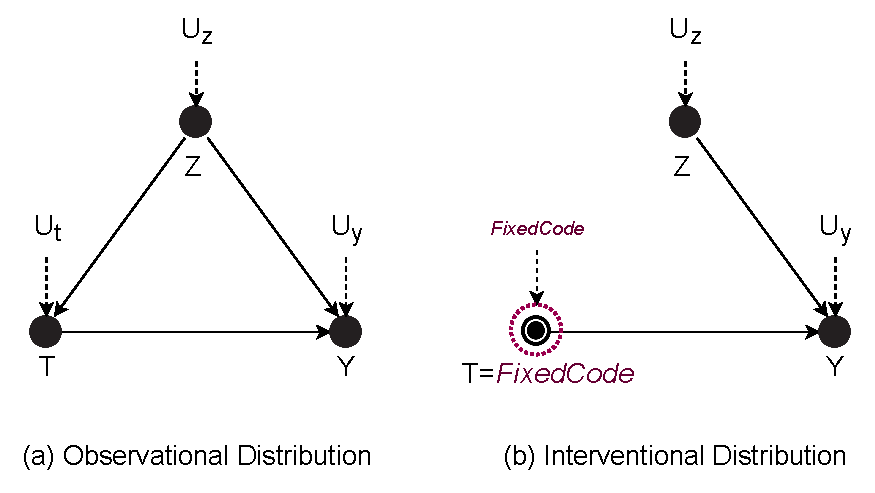
\includegraphics[width=0.9\textwidth]{graphics/preliminaries/fig_1_causalnet.pdf}
		\caption{(a) \textit{Structural Causal Model} representing cause-effect relationships of program repair in \nlms. (b) The \textit{SCM} after intervening the treatment with \textit{Fixed Code}.}
        \label{fig:scm}
\end{figure}

\begin{exmp} 
\label{exmp:scm}
Consider \figref{fig:scm} a generalization of the buggy influence on a deep model's performance. The first graph is a SCM composed of a treatment variable $T=Buggy$ and potential outcome $Y=Perf$. In addition, we identified some common causes $Z=SE_{Metrics}$ for treatments and potential outcomes. These common causes (or covariates) are Software Engineering quality metrics (\eg Lines of Code, McCabe Complexity, Size of Methods). Now we want to perform the intervention $do(Buggy=False)$ which is the same as $do(T=FixedCode)$. The second graph depicts this program repair intervention. Note that fixing the value of $T$ makes the SCM change by eliminating the effect or influence arrow of the common cause $Z$ to the treatment. The disturbance $U_t$ is also eliminated. This elimination process of input arrows to fixed variables is formally known as \textit{graph surgery}. Both $do(\cdot)-operator$ and graph surgery allow us to untangle causal relationships from mere correlations \citep{Pearl2009Causality}. The law of total probabilities and invariance principle are required to compute the observational and interventional distributions \citep{Scholkopf2022}:
\end{exmp}

\begin{subequations}
\begin{align}
p(Y|do(t=FixedCode)) &=\sum_{z \in _{metrics}}p(Y|z,t)p(t)\label{eqn:do-1} \\
p(Y|t=FixedCode) &= \sum_{z \in _{metrics}}p(Y|z,t)p(t|z) \label{eqn:do-2} 
\end{align}
\label{eqn:do-all-lines}
\end{subequations}

Note that \equaref{eqn:do-1} differs from  \equaref{eqn:do-2}: the prior $p(t)$ in contrast to $p(t|z)$, which is precisely the link that is eliminated in the SCM. \equaref{eqn:do-1} is formally known as the \textbf{\textit{adjustment formula}}. This formula is one of the building blocks in causal inference since it helps us to adjust common causes or control for covariates to compute the \textit{treatment or causal effect} \citep{Pearl2009Causality,Pearl2016Causality}.

\marginnote{
    \begin{definition}\label{def:effect}
    \textbf{Treatment Effects.} Given a Structural Causal Graph where a set of variables $PA$ denotes the parents of $T$, the treatment effect of T on Y is given by $p(Y=y|do(T=t))$ in Eq.~\ref{eq:effect}
    \end{definition}
}

\david{contextualize function below}
\begin{subequations}
    {%\tiny
        \begin{align}
        &p(Y=y|do(T=t)) &&=  \label{eq:effect-1}\\
        &\Sigma_z p(Y=y|T=t,PA=z)p(PA=z)  &&= \label{eq:effect-2}\\
        &\Sigma_z p(T=t,Y=y,PA=z)/p(T=t|PA=z) \label{eq:effect-3}
        \end{align}
    }
\label{eq:effect}
\end{subequations}

In our initial causal statement, we generally accept that buggy code \textit{causes} a \nlm to perform poorly. Although the causal statement is true, it is not guaranteed that every buggy snippet is certain to make a model perform poorly. Therefore, causal relationships are \textbf{uncertain}. This uncertainty is captured by employing conditional probabilities described in \equaref{eq:effect-1}. In order to compute treatment effects, we need to connect observational data with our interventional distribution. Note \equaref{eq:effect-3} is obtained with Bayes' rule and algebraic manipulation once we multiply and divide by the term $p(T=t|PA=z)$. This term is a conditional probability known as the \textit{propensity score}. This propensity score and the join probability of all the nodes are distributions that can be obtained from data \citep{Pearl2016Causality}. We explain this connection for code generation in \secref{sec:approach-hbn}. 

\david{Re-write the following paragraph to generalize the thesis document.}
In summary, our interpretability methodology \codegen is based on the idea of proposing causal queries given a SCM. These causal queries are obtained by estimating an interventional distribution where the potential outcome is generally a prediction performance value of Neural Code Model under study and the treatments are a set of software-based properties that help us construct explanations about the generative model.

%------------------------------------------------

%\input{chapters/chap_03_causality/sec_02_causal-information} %<----- TO BE INCLUDED



%----------------------------------------------------------------------------------------
%	PART I: CAUSALITY APPLICATIONS I. DEEP CODE RETRIEVAL
%----------------------------------------------------------------------------------------

\part{Causality Applications I. Deep Code Retrieval}

%----------------------------------------------------------------------------------------
%	CHAPTER 4: DEEP CODE RETRIEVAL BAYES
%----------------------------------------------------------------------------------------

\chapter{Inferring Trace Links with \break a Hierarchical Bayesian Network}
\label{ch:hbn}

% 0. A General Introduction

The importance of traceability in modern software systems cannot be overstated. Traceability links that connect ``high-level" artifacts such as requirements and use cases to ``low-level'' artifacts written in code help to facilitate crucial components of the software development and maintenance cycle. For instance, linking requirements to code provides visibility into a system by enumerating what has been implemented, whereas linking requirements to test cases helps to provide an indication that the software is functioning as expected. Additionally, the establishment of trace links aids in facilitating a broad set of developer activities including code comprehension, change impact analysis, and compliance validation~\citep{Cleland-Huang:Springer'12}.  In certain software domains, such as those involving safety critical systems, traceability is necessarily \textit{mandated} by regulatory bodies in order to properly demonstrate the safe functioning of a system~\citep{Nejati:IST'12,Rempel:ICSE'14,Cleland-Huang:ICSE'10,Mader:Soft'13}. Furthermore, traceability is increasingly used to help ensure the \textit{security} of a given system~\citep{Nhlabatsi:SST'15}. For example, our industrial partners at Cisco Systems, Inc. require that security-critical requirements are verified by a dedicated group of analysts to avoid software threats and ensure best practices. 

Unfortunately, despite its importance, software traceability is, by its nature, an inherently difficult and error prone task~\citep{Cleland-Huang:FOSE'14,Mahmoud:ICPC'12,Mader:Soft'13}. This difficulty primarily stems from the need to bridge a logical abstraction gap that exists between different software artifacts, such as requirements written in natural language and code written in ``lower-level'' programming languages.  %Thus, bridging this abstraction gap typically requires developers or analysts with expertise related to a given software system to manually comprehend these artifacts and decipher meaningful relationships among them.  
Given the effort required to establish and evolve effective trace links, it is often too costly to manually establish them outside of regulated domains, and in practice the quality of mandated links are often questionable~\citep{Cleland-Huang:FSE'14}.  

The inherent difficulty in establishing trace links has lead to research on automated techniques for modeling, establishing, and evolving trace links that primarily rely upon information retrieval (IR)~\citep{Lucia:ICSM'04,Dekhtyar:RE'07,Asuncion:ICSE'10,McMillan:TEFSE'09,Gethers:ICSM'11,DeLucia:ASE'08,DeLucia:EMSE'09,Mahmoud:ICPC'12,Antoniol:ICSE'00,Marcus:ICSE'03,Mills:ICSME18,Jiang:ASE'08,Kuang:SANER'17} and machine learning (ML)~\citep{Mahmoud:RE'16,Guo:MSR'16,Asuncion:ICSE'10,Spanoudakis:SEKE'03,Falessi:EMSE17} techniques which retrieve or predict trace links based upon textual similarity metrics.  However, in large part, current automated approaches for traceability often trade precision for completeness and vice versa, making them difficult to adopt in practice. We observe three major shortcomings of current automated techniques that contribute to their limited effectiveness:

\noindent{\textbf{1) Limited Measures of Artifact Similarity:}} Existing techniques for trace link recovery tend to use a single textual similarity metric to draw relationships between artifacts. This is problematic for several reasons. Perhaps most importantly, it is often difficult or impossible to determine how well a technique that uses a given similarity measure will function on artifacts from a new project without any pre-existing trace links. This so-called ``cold-start'' problem is due to the fact that existing IR/ML techniques for measuring textual similarity often need to be calibrated on a subset of "ground-truth" artifact pairs with pre-existing links. This makes performance of these techniques difficult to predict when applied to new datasets. Furthermore, in practice industrial projects often lack pre-existing trace links, as confirmed by our  partners at Cisco. Thus, while certain techniques have been shown to perform well on research benchmarks, the efficacy of a similarity measure is often tightly coupled to the underlying semantics of software artifact text~\citep{Lohar:FSE'13,Guo:ICSE'17,Biggerstaff:ACM'94}, and to the configuration of the corresponding IR/ML technique~\citep{Oliveto:ICPC'10}. 

Using only a single textual similarity metric also needlessly restricts the predictive power of a traceability technique. Past work has illustrated the orthogonality of different similarity measures~\citep{Oliveto:ICPC'10}, suggesting that combining \textit{several} different measures could lead to more accurate and robust techniques that function \textit{consistently} well when applied to new projects without pre-existing links.

\noindent{\textbf{2) Inability to Effectively Capture Developer Feedback:}} The rapid pace of modern agile development practices often results in crucial knowledge about a software system being siloed within the expertise of individual developers. Thus, one unstructured development artifact that has gone underutilized by past techniques is \textit{developer feedback}. When an automated traceability model is uncertain about particular trace link pairs, developers can provide critical feedback to help improve trace link inference.

\noindent{\textbf{3) Limited View of Interactions Between Artifacts}}
Existing automated traceability approaches are typically tailored to establish relationships between pairs of specific types of artifacts (\eg user stories and class files). However, information pertaining to the relationship of one type of artifact pair may be contained within other related artifacts. For example, if a piece of source code is linked to a given requirement through textual similarities, and this source code is also intrinsically linked to test code via method calls, then it is likely the requirement is also linked to the test code. However, in this situation, it may be difficult for a textual similarity metric to link the requirements and test code, due to limited test documentation, for example. Thus, in this way, established relationships between certain artifacts may influence the probability of other artifact relationships. In this paper we refer to these phenomena as \textit{transitive links}. Existing techniques generally cannot model such interactions between artifacts.

The limitations discussed above stem from both technical and practical limitations of existing traceability techniques, and surfaced during our development of an automated traceability approach in close collaboration with Cisco Systems. In this paper we introduce a novel technique that overcomes these limitations by constructing a Hierarchical Bayesian Network for inferring a set of candidate trace links. The model that underlies our approach is capable of deriving the probability that a trace link exists between two given artifacts by combining information from multiple measures of textual similarity, while simultaneously modeling transitive relationships and accounting for developer expertise.  We implemented our approach, called \Comet (Hierarchi\textbf{C}al Pr\textbf{O}babilistic \textbf{M}odel for Softwar\textbf{E} \textbf{T}raceability), in both an extensible Python library and as a plugin for the popular Jenkins CI/CD system.  In an extensive set of empirical experiments we illustrate that \Comet is able to outperform the median precision of \textit{optimally configured} baseline techniques by $\approx$5\% across subjects and $\approx$14\% in the best case. Given that optimal configuration is typically not possible in practice, this illustrates that given a project with no pre-existing trace links, \Comet is likely to perform significantly better than most existing IR/ML techniques. Additionally, we show \Comets potential for integration into the workflows of development teams at Cisco. In summary, this paper's contributions are as follows \david{Fix this contributions to be more precise for the chapter}:

\begin{itemize}
	\item{The derivation of a Hierarchical Bayesian Network (HBN) for inferring a candidate set of trace links;}	
	\item{An implementation of this model, called \Comet, as both an extensible Python library and a Jenkins plugin that has been deployed for testing with our industrial partners at Cisco;}
	\item{An extensive evaluation of \Comet on both open source projects and two industrial datasets from one industrial software project, including feedback from professional developers at a major telecommunication software company;}
	\item{An open source, commercial-grade traceability benchmark, developed in coordination with our industrial partner, for the benefit of the research community;}
	\item{An online appendix, including our open source implementation of \Comet and evaluation data for reproducibility~\cite{appendix}}.
\end{itemize}

%------------------------------------------------

\section{The Hierarchical Bayesian \hfill \break Software Retrieval Model}
\label{sec:approach-hbn}

In this section, we provide a formal description of \Comets probabilistic model introduced at a high level in \secref{subsec:model-motivation} \david{Check This reference}. To help aid in the comprehension of \Comets underlying model, we provide a graphical representation using plate notation~\citep{Murphy:2012} in \figref{fig:model-approachI}, which we use to guide our introduction and discussion. The model in \figref{fig:model-approachI} is computed on a \textit{per link} basis, that is between all potential links between a set of source ($S$) and target artifacts ($T$). In this section we will use $S_x$ and $T_y$ to refer to a single source and target artifact of interest respectively. \Comets probabilistic model is formally structured as an HBN, centered upon a \textit{trace link prior} $\theta$ which represents the model's prior belief about the probability that $S_x$ and $T_y$ are linked.  Our model is hierarchical, as the trace link prior is influenced by a number of \textit{hyperpriors}, which are constructed in accordance with a set of \textit{hyper-parameters} that are either derived empirically, or fixed. In \figref{fig:model-approachI}, hyperpriors are represented as empty nodes, and hyper-parameters are represented as shaded blue nodes. In general, empty nodes represent latent, or hidden, variables whereas shaded nodes represent variables that are known or empirically observed quantities. The rectangles, or ``plates'' in the diagram are used to group together variables that repeat.

\begin{marginfigure}%[tb]

\centering
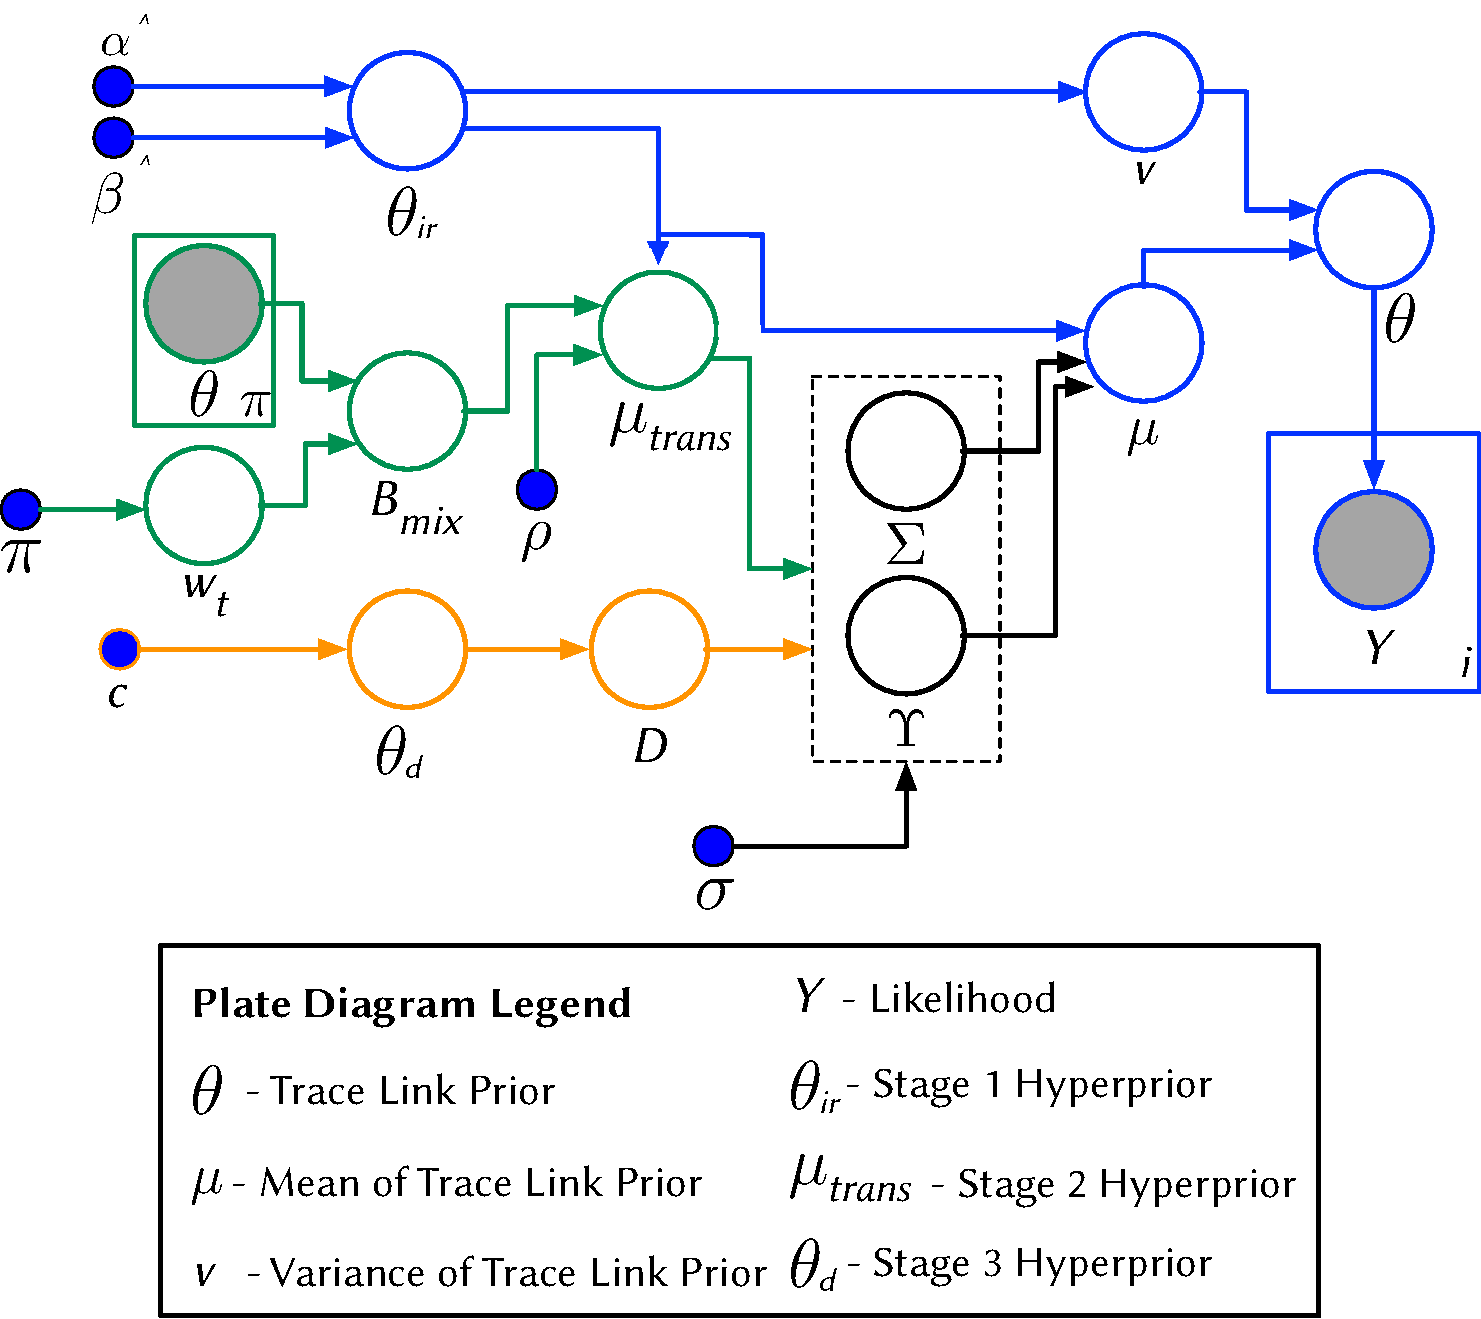
\includegraphics[width=\columnwidth]{graphics/chap_04-bayes/fig1_Model-Plate-Diagram.pdf}
\caption{Plate Diagram of \Comets HBN}
\label{fig:model-approachI}

\end{marginfigure}

To make our model easier to comprehend, we have broken it down into four major configurations, which we call \textit{stages}, indicated by different colors in \figref{fig:model-approachI}. The first stage of our model (shown in blue at top) unifies the collective knowledge of textual similarity metrics computed by IR/ML techniques. The second stage (shown in orange at the bottom) reconciles expert feedback to improve the accuracy of inferred trace links. The third stage (shown in green in the middle) accounts for transitive relationships among development artifacts, and the fourth stage combines each of the underlying stages. It should be noted that the first stage of our model can be taken as the ``base case'' upon which the other complexities build and is always required to infer the existence of a trace link.  The order of calculation starts with the first stage and proceeds sequentially. The design and parameterization of our model presented in this section is not arbitrary, but instead based on the well-founded theory of \textit{conjugate priors}~\citep{Raiffa:61} which aids in defining appropriate distributions and hyperparameters for a given prior. We center the description of our model first upon the likelihood estimation and then around the estimation of the prior probability distribution as defined by the four stages. After defining the hyperpriors for each of the four stages we briefly discuss the inference techniques we employ to estimate the posterior probability distribution of our model and thus the probability of whether a given link exists. While this section provides an overview of our model, we discuss its instantiation (including utilized IR/ML techniques) in \secref{subsec:exp-context} \david{fix the reference}.

%------------------------------------------------

\subsection{Estimating the Likelihood}
\label{sub:model-likelihood}

The likelihood function in our HBN models observed data so that these observations can be reconciled with our estimated prior probability distribution to infer a posterior probability.  The likelihood is shown as the observed variable $Y$ (\figref{fig:model-approachI}). The variable $i$ represents the number of observations made. In the context of traceability, we express the likelihood as a discrete Bernoulli distribution, as two artifacts can either be ``linked'' or ``not-linked'':

\begin{equation}\label{eq:likelihood}
Y = p(l_i|\theta_i)= Bern(l_i|\theta_i)
\end{equation}

\noindent \david{fix this} where $l_i$ is an observable data point ${0,1}$ for $i$ number of observations. We define an observation as a function of the textual similarity score generated by an IR technique between $S_x$ and $T_y$ and some threshold $k_i$ where any similarity above the threshold is considered an observed link, and any similarity value below this threshold is considered a non-link. The number of IR techniques or configurations utilized corresponds to the number of observations $i$.  Ideally, to capture the most accurate trace link observations from IR techniques, the threshold $k_i$ should be chosen to maximize the chance that each IR technique correctly establishes whether two artifacts are linked.  In other words, $k_i$ should be chosen for each IR technique such that the precision and recall of the technique is maximal across the entire set of considered source and target artifacts $S$ and $T$.  However, this information is not available a-priori without the consultation of a ground truth set of trace links. As we illustrate in \secref{sec:study} \david{fix this reference} this threshold can often be estimated with surprising accuracy by analyzing the distribution of similarity values an IR technique produces for a given set of artifacts. 

%-------------------------------

\subsection{Stage 1 - Unifying Textual Similarities between Development Artifacts}
\label{sub:model-comp1}

The first ``base'' stage of our model informs the trace link prior, represented as a probability distribution $p(\theta)$, according to the textual similarity measurements of a set of IR techniques.  However, converse to the likelihood estimation, the actual textual similarity values of IR techniques are directly used to estimate a Beta distribution (the conjugate prior of the likelihood's Bernoulli distribution). This Beta distribution is represented as follows: 

\begin{equation}\label{eq:lvl1-dist}
\theta \sim B(\mu, \nu) 
\end{equation}

\noindent where $\mu$ and $\nu$ are parameters of the Beta distribution representing its mean and variance. This prior, and its two parameters are illustrated in the right-most part of the blue segment (\figref{fig:model}). To inform this Beta distribution, the textual similarity of values of a given number $i$ of IR/ML techniques are normalized according to a sigmoid function centered upon the median of the distribution of similarity values across all $S$ and $T$ in a given dataset. Then a logistic regression is performed upon the normalized similarity values to infer the values $\hat{\alpha}$ and $\hat{\beta}$ which define a hyperprior beta distribution $\theta_{IR}$. This hyperprior with parameters are shown on the left of the blue segment (\figref{fig:model}). The mean and the variance of this hyperprior distribution then inform $\mu$ and $\nu$ of the base prior $\theta$:


\begin{equation}\label{eq:lvl1-params}
\nu = Var[\theta_{IR}] \quad \mu = Mean[\theta_{IR}]
\end{equation}

Thus, by considering the textual similarity values of a set of IR techniques, our model can effectively reconcile the collective knowledge to ultimately make an informed prediction.

%-------------------------------
\subsection{Stage 2 - Incorporating Developer Feedback}
\label{sub:model-comp2}

The second stage of our model is capable of leveraging human feedback by influencing the prior distribution introduced in the first stage of our model. To model expert feedback, we estimate hyperpriors $D$ and $\theta_d$, shown in orange in \figref{fig:model}. To perform this estimation, our model accepts from a developer or analyst, their confidence that a given link exists as a value between $[0,1]$. In \secref{subsec:comet-jenkins} \david{fix it} we illustrate how such feedback can be collected from developers in a lightweight manner. This confidence value serves as a parameter for estimating the distribution of the first hyperprior:

\begin{equation}
\theta_{d} \sim B(\mu_{d}=c,sd=0.01)	
\end{equation}

\noindent where $\theta_{d}$ is a Beta distribution parameterized by its mean $\mu_d$ set to the confidence value provided by a developer, and standard deviation $sd$ which we set to 0.01 signaling a low variance in the derived Beta distribution. This distribution then parameterizes the second hyperprior $D$, modeled as a Bernoulli distribution.

Now that we have derived a distribution representing developer feedback, we must define how this distribution affects the prior probability of the first stage of our model. To do this, we define reward and penalty functions $\Upsilon$ and $\Sigma$ that are influenced by $\sigma$ which represents a specified \textit{belief factor} between $[0,1]$ that controls the extent to which the feedback influences the trace link prior. The reward function is defined as $\Upsilon = \sigma*D$, whereas the penalty function is defined as $\Sigma = \sigma*(D-1)$. These factors impact the first stage prior Beta distribution by affecting its mean $\mu$:

\begin{equation}\label{eq:mean-affect}
	\mu \sim N(\mu_n= \Sigma + \Upsilon, sd=0.01)
\end{equation}

\noindent where the mean of the first stage prior is represented as a normal distribution parameterized by $\mu_n$ set to the sum of $\Sigma$ and $\Upsilon$, and a standard deviation set to 0.01. Thus, in this manner, expert feedback is utilized to influence the prior distribution that a given trace link exists. The structure of the Stage 2 hyperpriors allows \Comets HBN to effectively consider feedback from multiple developers.

%-------------------------------
\subsection{Stage 3 - Leveraging Transitive Links}
\label{sub:model-comp3}

As discussed earlier, the probability that a trace link exists between a source and target artifact can be influenced by \textit{transitive} relationships among varying software development artifacts.  The third stage of \Comets HBN is able to utilize these transitive links to improve the accuracy of its inferred trace link. However, before we describe how our model reconciles this information in a probabilistic manner, it is first important to understand the phenomena of transitive links. At a high level, a transitive link is an inherent relationship between two software artifacts ($A_1$,$A_2$) that may influence the existence of a trace link between either $A_1$ and any other artifact or $A_2$ and any other artifact. \Comet is currently capable of leveraging two types of transitive links, one based on textual-similarities (req. $\leftrightarrow$ req.) and one based on dynamic execution information (req. $\leftrightarrow$ test case). However, \Comet could also be extended to model transitive relationships between other types of artifacts, such as commit messages or issues. \figref{fig:trans-req2req} provides an illustration of both transitive link types, which we detail below. Note that for execution traces, a relationship is considered \textit{strong} between a test method and source method if the test executes the method, and \textit{weak} otherwise. For req$\leftrightarrow$req relationships, it is \textit{strong} if the textual similarity is above the threshold $\tau$, and \textit{weak} if it is below the threshold.

\begin{figure}%[tb]
\centering
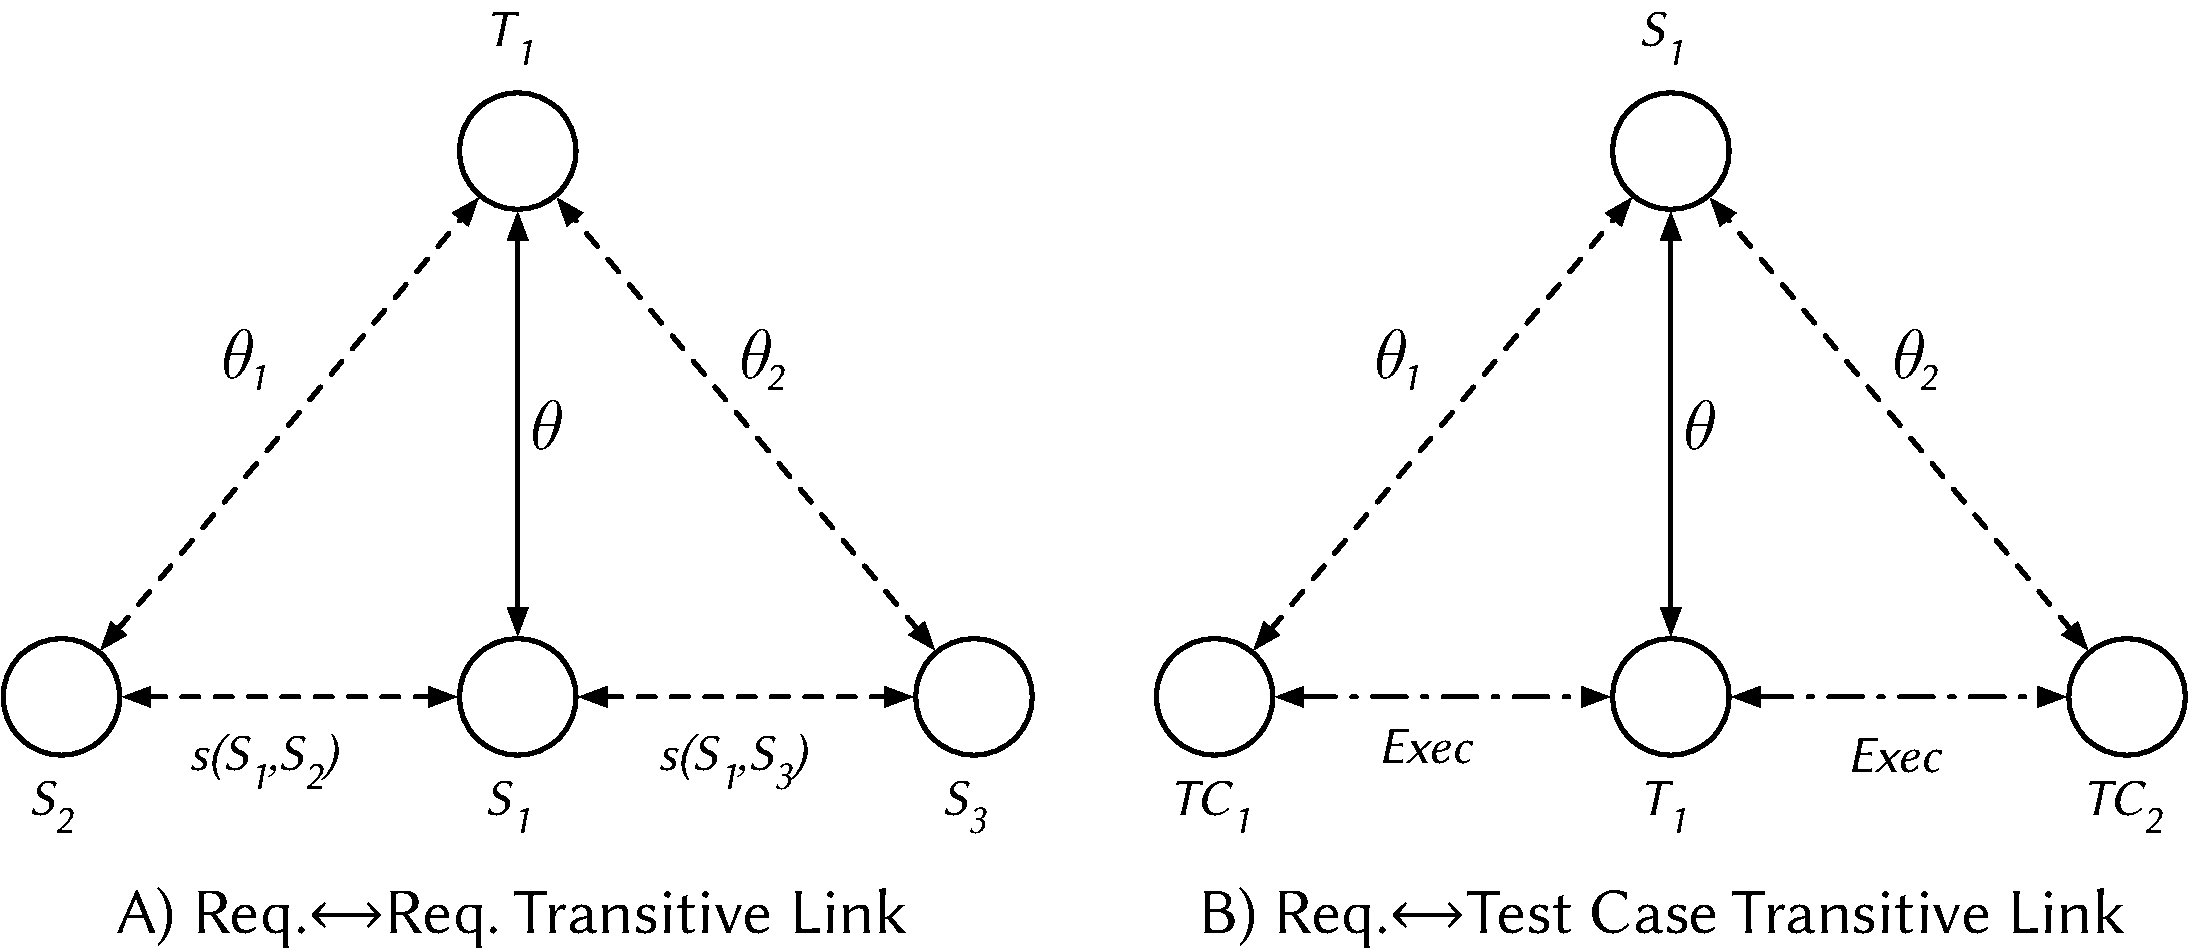
\includegraphics[width=\columnwidth]{graphics/applicationsI-approach/fig2_transitive-links.pdf}
\caption{Illustration of Transitive Links}
\label{fig:trans-req2req}
\end{figure}

{\textbf{Req. $\leftrightarrow$ Req. Links}} Consider $S_1,S_2,S_3$ as three source artifacts representing three discrete requirements documents and $T_1$ is a potential target document (\ie source code file), where the target relationship being inferred is $S_1\rightarrow T_1$, indicated by the solid line. The connections between nodes denote relationships among the artifacts. Consider the scenario in which the relationship between $S_1$ and $T_1$ is weak, but $S_1$ is highly similar to the other two requirements $S_2$ and $S_3$. Given that we know the three source artifacts are highly related, the relationships between $S_2\rightarrow T_1$ and $S_3\rightarrow T_1$ have a \textit{transitive} influence on the target relationship between $S_1$ and $T_1$. For instance, if $S_2\rightarrow T_1$ and $S_3\rightarrow T_1$ both indicate strong probabilities, then likewise the probability of the target link $S_1\rightarrow T_1$ should be increased to account for these transitive relationships.

{\textbf{Req.$\leftrightarrow$ Test Case Links}} Consider $S_1$ to be a source artifact representing a requirement document, $T_1$ to be a potential target source code file, and $TC_1,TC_2$ to be test cases, where the target relationship being inferred is $S_1\rightarrow T_1$, indicated by the solid line. Consider again the scenario in which the relationship between $S_1$ and $T_1$ is weak, whereas the relationship between $S_1$ and $TC_1,TC_2$ are stronger. If we observe that $TC_1$ and $TC_2$ are related to $T_1$ by execution information (\eg $TC_1$ and $TC_2$ both exercise $T_1$, \textit{Exec} in Fig. \ref{fig:trans-req2req}) then, this transitive relationship should influence the probability that a trace link exists between $S_1$ and $T_1$.

{\textbf{Incorporating Transitive Links into C{\footnotesize OMET}'s HBN}} In order for our HBN to incorporate transitive req. $\leftrightarrow$ req. links, it must first derive the set of requirements that are related to a given target requirement $S_x$. To accomplish this, one of several IR techniques can be used to compute textual similarity, or the first stage of our model can be used to derive the relationships, illustrated as $s(S_1,S_2)$ \& $s(S_1,S_3)$ in Fig. \ref{fig:trans-req2req}. To incorporate information from req. $\leftrightarrow$ test case links, dynamic information must be collected that provides the $Exec_1$ \& $Exec_2$ relationships illustrated in Fig. \ref{fig:trans-req2req}. In either case, a specified threshold $\tau$ signals whether a pair of requirements is related, and the total number of related requirements or test cases is specified by the hyper-parameter $\pi$.  Once the related requirements have been derived, our HBN estimates three hyperpriors, $w_t$, $B_{mix}$ and $\mu_{trans}$. First $w_t$ is formulated as a Dirichlet distribution according to the number of related transitive requirements. Then to estimate $B_{mix}$, the first stage of our HBN is computed between each related requirement and a given target artifact $T_y$. The inferred values for each transitive link, and $w_t$ are used to form a mixture model:

\begin{equation}
	B_{mix} \sim Mix(w_t,\theta_\pi)
\end{equation}

\noindent where $B_{mix}$ is a Beta mixture model parameterized by the 1st stage inference of each transitive link and $\pi$ weights modeled as a Dirichlet distribution parameterized by $\pi$. This Dirichlet distribution is then used to derive a meditated normal distribution $\mu_{trans}$:

\begin{equation}
	\mu_{trans} \sim \rho*B_{mix} + (1-\rho)*Mean[\theta_{IR}]
\end{equation}

\noindent where $Mean[\theta_{IR}]$ represents the mean of the probability distribution of IR similarity values (from stage 1) on the trace link prior and $\rho$ is represents the \textit{belief factor} of the transitive links (\eg the degree to which the transitive relationships should affect overall prior trace link probability). $\mu_{trans}$ can then be utilized to derive the reward and penalty functions introduced earlier where $\Upsilon = \sigma*(1-\mu_{trans})$ whereas $\Sigma = \sigma*\mu_{trans}$. The reward and penalty functions can then in turn be used to influence the mean of trace link prior $\mu$:

\begin{equation}\label{eq:mean-affect-combined}
	\mu \sim N(\mu_n= \mu_{trans} + \Sigma + \Upsilon, sd=0.01)
\end{equation}

\noindent in the same manner as introduced in Eq. \ref{eq:mean-affect}. In this way, our model is capable of incorporating information from transitive links, increasing the overall prior probability if transitive links are strongly connected to the target artifact $T_y$ and decreasing it if they are not strongly connected.

%-------------------------------
\subsection{Stage 4 - The Holistic Model}
\label{sub:model-comp4}

The holistic model combines all three underlying stages. To accomplish this, the calculations of the reward and penalty functions for affecting the mean $\mu$ of the overall prior are modified to incorporate information from both expert feedback and transitive links:

\begin{align}
\begin{split}
	\Upsilon \sim (1-\mu_{trans})*\sigma*D \\
	\Sigma \sim \mu_{trans}*\sigma*(D-1)
\end{split}
\end{align}

\noindent Then Eq. \ref{eq:mean-affect-combined} can be used to derive the new mean for the overall prior probability distribution of the model.

%-------------------------------
\subsection{Inferring the Posterior}
\label{sub:model-posterior}

In order to reason about the probability that a trace link exists, we must estimate the posterior probability distribution of our hierarchical model $p(\Theta|L)$ according to the observable data $L$ and prior knowledge of the link $p(\Theta)$. Here $p(\Theta)$ encompasses the trace link prior and all constituent hyperpriors depending upon the stage of the model.  Once the posterior has been estimated, \Comet utilizes the \textit{mean} of the distribution as the general probability that a link exists. We can represent the general calculation of the posterior for our model using using Bayes Theorem as follows:  

\vspace{-0.3cm}
\begin{equation} \label{eq_bayes}
p(\Theta|L) = \dfrac{p(\Theta)p(L|\Theta)}{\int p(\Theta)p(L|\Theta)d\Theta} \propto p(\Theta) \prod\limits_{i=1}^n p(L_i|\Theta_i)
\end{equation}

\noindent where $n$ represents the total number of observations (\ie the number of underlying IR techniques and configurations).  \Comets HBN is non-trivial, and thus the posterior $p(\Theta|L)$ cannot be computed analytically. Therefore, we turn to approximation techniques for estimating the posterior probability distribution. Comet can currently utilize three different techniques including (i) Maximum a Posteriori (MAP) estimation~\citep{Bassett2018MaximumEstimators}, a Markov Chain Monte Carlo (MCMC) technique via the No-U-Turn sampling (NUTS) process~\citep{Hoffman2011TheCarlo}, and a machine learning-based technique called Variational Inference (VI)~\citep{Bishop:2006}. We provide experimental results in \secref{sec:results} for all techniques for Stage 1 of \Comets model, and NUTS/MAP for Stages 2-4, as VI cannot be applied to more complex stages of the model.

\subsection{Experimental Context}
\label{sub:exp-context}

\textbf{Subject Datasets}

%------------------------------------------------

\section{Design}
\label{sec:design-hbn}

To evaluate \Comet, we perform an extensive empirical evaluation with two major \textit{goals}: (i) evaluate the effectiveness of the four stages of \Comets HBN in terms of their ability to effectively infer trace links, and (ii) examine whether \Comet is applicable in industrial workflows. The \textit{quality focus} of our study is \Comets effectiveness, in terms of generating an accurate and complete set of trace links, and practical applicability. We formulate the following set of RQs:

\begin{itemize}

	\item{\textbf{RQ$_1$}: \textit{How effective is \Comet at inferring candidate trace links using combined information from IR/ML techniques?}}

	\item{\textbf{RQ$_2$}: \textit{To what extent does expert feedback impact the accuracy of the candidate trace links of \Comet?}}

	\item{\textbf{RQ$_3$}: \textit{To what extent does information from transitive links improve \Comets trace link inference accuracy?}}

	\item{\textbf{RQ$_4$}: \textit{How effective is the holistic \Comet model in terms of inferring candidate trace links?}}

	\item{\textbf{RQ$_5$}: \textit{Do professional developers and security analysts find our implementation of the \Comet Jenkins plugin useful?}}
	
\end{itemize}

%------------------------------------------------
\subsection{Experimental Context}
\label{sub:exp-context}

\begin{table}[h]
\centering
\caption{Datasets used for \Comets evaluation. Req = Requirement, Src = Source code, UC = Use Case}
\label{tab:datasets-hbn}

%\scalebox{0.8}{%
\resizebox{\textwidth}{!}{

\begin{tabular}{@{}llccccc@{}}
\toprule
\multicolumn{1}{c|}{\textbf{Dataset}} &
  \multicolumn{1}{c|}{\textbf{Language}} &
  \multicolumn{1}{c|}{\textbf{Size (LoC)}} &
  \textbf{\begin{tabular}[c]{@{}c@{}}\#Source \\ Artifacts\end{tabular}} &
  \textbf{\begin{tabular}[c]{@{}c@{}}\#Target\\ Artifacts\end{tabular}} &
  \multicolumn{1}{c|}{\textbf{\begin{tabular}[c]{@{}c@{}}\#Pairs \\ (\#Links)\end{tabular}}} &
  \textbf{Type} \\ \midrule
\multicolumn{7}{c}{\textbf{Training Datasets}}                                                                                                           \\ \midrule
\multicolumn{1}{l|}{Albergate} & \multicolumn{1}{l|}{Java}      & \multicolumn{1}{c|}{10,464} & 55  & 17  & \multicolumn{1}{c|}{935/53}    & Req $\to$ Src  \\
\multicolumn{1}{l|}{EBT}       & \multicolumn{1}{l|}{Java}      & \multicolumn{1}{c|}{1,747}  & 40  & 25  & \multicolumn{1}{c|}{1000/51}   & Req $\to$ Test \\ \midrule
\multicolumn{7}{c}{\textbf{Experimental Datasets}}                                                                                                       \\ \midrule
\multicolumn{1}{l|}{\multirow{2}{*}{LibEST}} &
  \multicolumn{1}{l|}{\multirow{2}{*}{C}} &
  \multicolumn{1}{c|}{\multirow{2}{*}{70,977}} &
  59 &
  11 &
  \multicolumn{1}{c|}{649/204} &
  Req $\to$ Src \\
\multicolumn{1}{l|}{}          & \multicolumn{1}{l|}{}          & \multicolumn{1}{c|}{}       & 59  & 18  & \multicolumn{1}{c|}{1062/352}  & Req $\to$ Test \\
\multicolumn{1}{l|}{eTour}     & \multicolumn{1}{l|}{Java}      & \multicolumn{1}{c|}{23,065} & 58  & 116 & \multicolumn{1}{c|}{6728/308}  & UC $\to$ Src   \\
\multicolumn{1}{l|}{EBT}       & \multicolumn{1}{l|}{Java}      & \multicolumn{1}{c|}{1,747}  & 40  & 50  & \multicolumn{1}{c|}{2000/98}   & Req $\to$ Src  \\
\multicolumn{1}{l|}{SMOS}      & \multicolumn{1}{l|}{Java}      & \multicolumn{1}{c|}{9,019}  & 67  & 100 & \multicolumn{1}{c|}{6700/1044} & UC $\to$ Src   \\
\multicolumn{1}{l|}{iTrust}    & \multicolumn{1}{l|}{Java, JSP} & \multicolumn{1}{c|}{38,087} & 131 & 367 & \multicolumn{1}{c|}{48077/399} & Req $\to$ Src  \\ \bottomrule
\end{tabular}
}

\end{table}

\textbf{Subject Datasets.} The \textit{context} of this empirical study includes the eight datasets shown in \tabref{tab:datasets-hbn}. Six of these are taken from the open source CoEST community datasets~\cite{coest-datasets}. These datasets represent a set of benchmarks created by the research community and widely used as an effective assessment tool for automated traceability techniques~\citep{Antoniol:e,Cleland-Huang:TSE'03,Poshyvanyk:TEFSE'11,Gethers:ICSM'11}. In order to maintain the quality of our experimental subjects, we do not use all available projects in the CoEST repository, as we limited our studied systems to those that: (i) included trace links from requirements or use cases written in natural language to some form of code artifact, (ii) were written in English and/or included English translations, and (iii) had at least 1k LoC.  We utilize two datasets to investigate and tune the hyper-parameters of \Comets HBN, Albergate, and the Rq$\rightarrow$Tests dataset of the EBT project. We utilize the other six datasets for our empirical evaluation. The subject system called ``LibEST'' is an open source networking related software project, which was created and is actively maintained by engineers at Cisco as an implementation of RFC-7030 ``Enrollment over Secure Transport''. We derived the ground truth set of trace links between Rq$\rightarrow$Src and Rq$\rightarrow$Tests for this dataset in close collaboration with our industrial partner. First, one of the authors carefully created an initial set of trace links. Then, an engineer working on the project reviewed the links and confirmed or denied a subset, based on their availability. The author then revised the links using the engineer's feedback, and this process continued over several months until the ground truth was established. The "LibEST" dataset is available along with all of our experimental data to facilitate reproducibility~\citep{appendix}.

%------------------------------------------------

\textbf{Studied IR Techniques.} The ``base'' first stage of \Comets HBN is able to utilize and unify information regarding the textual similarity of development artifacts as computed by a set of IR/ML techniques.  While there is technically no limit to the number of IR/ML techniques that can be utilized, we parameterized our experiments using ten IR-techniques enumerated in \tabref{tab:ir-techniques-hbn}. The first five techniques are standalone techniques, whereas the second five are combined techniques utilizing the methodology introduced by Gethers \etal~\citep{Gethers:ICSM'11}. This combined approach normalizes the similarity measures of two IR techniques and combines the similarity measures using a weighted sum. We set the weighting factor $\lambda$ for each technique equal to 0.5, as this was the best performing configuration reported in the prior work~\citep{Gethers:ICSM'11}. We explain the differences between the technique employed by Gethers et. al. and \Comet in \secref{sec:discussion-hbn}. The other parameters for each of the techniques were derived by performing a series of experiments on the two tuning datasets, and using the optimal values from these experiments. For all IR techniques, we preprocessed the text by removing non-alphabetic characters and stop words, stemming, and splitting camelCase. We performed 30 trials for each technique involving LDA, and chose the number of topics that led to optimal performance on our tuning projects. To aid in experimental reproducibility, complete configurations for each technique are listed in our online appendix~\citep{appendix}.



\begin{margintable}
\centering
\caption{IR/ML Techniques used in the Construction of C{\tiny OMET}'s HBN}
\label{tab:ir-techniques-hbn}
\scalebox{0.7}{%

\begin{tabular}{@{}l|c|c@{}}
\toprule
\multicolumn{1}{c|}{\textbf{\begin{tabular}[c]{@{}c@{}}Information Retrieval \\ Technique\end{tabular}}} &
  \textbf{Tag} &
  \textbf{\begin{tabular}[c]{@{}c@{}}Treshold \\ Technique\end{tabular}} \\ \midrule
Vector Space Model          & VSM     & Link-Est \\
Latent Semantic Indexing    & LSI     & Link-Est \\
Jensen-Shannon Divergence   & JS      & Min-Max  \\
Latent Dirichlet Allocation & LDS     & Min-Max  \\
\begin{tabular}[c]{@{}l@{}}NonNegative \\ Matrix Factorization\end{tabular} &
  NMF &
  Median \\
Combined VSM + LDA          & VSM+LDA & Link-Est \\
Combined JS+LDA             & JS+LDA  & Link-Est \\
Combined VSM+NMF            & VSM+NMF & Link-Est \\
Combined JS+NMF             & JS+NMF  & Link-Est \\
Combined VSM+JS             & VSM+JS  & Min-Max  \\ \bottomrule
\end{tabular}

}
\end{margintable}


%------------------------------------------------

\subsection{RQ$_1$: C{\footnotesize OMET} Performance w/ Combined IR/ML Techniques}
\label{sub:study-rq1}

To answer RQ$_1$, we ran the first stage of \Comets HBN on our six evaluation datasets using the ten IR/ML techniques enumerated in Table \tabref{tab:ir-techniques-hbn}. However, as explained in \secref{subsec:model-comp1}, in order to accurately estimate the likelihood function $Y$ we need to choose a threshold $k_i$ for each IR technique that maximizes the precision and recall of the trace links according to the computed textual similarity values. To derive the best method for determining the threshold for each IR technique, we performed a meta evaluation on our two tuning datasets. We examined five different threshold estimation techniques: (i) using the mean of all similarity measures for a given dataset, (ii) using the median of all similarity measures across a given dataset, (iii) using a Min-Max estimation, (iv) a sigmoid estimation, and (v) link estimation (Link-Est), where an estimation of the number of confirmed links for a dataset is made based on the number of artifacts, and a threshold derived to ensure that the estimated number of links is above that threshold.  We performed each of these threshold estimation techniques for all studied IR techniques across our two tuning datasets, and compared each estimation to the known optimal threshold. We used the optimal technique across our two tuning datasets, as reported in \tabref{tab:ir-techniques-hbn}. To aid in reproducibility, we provide a detailed account of these experiments in our online appendix~\citep{appendix}.

To provide a comparative baseline against which we can measure \Comets performance, we report results for the best-performing and median of the studied IR/ML techniques, optimally configured for each dataset. We chose to optimally configure the baseline techniques, even though such configurations would not be possible in practice due to the absence of a ground truth, in order to illustrate how close Comet can come to the ``best-case baseline scenario''. 

To provide a comprehensive comparison of \Comet to a state of the art technique for candidate trace link generation, we re-implemented the DL-based approach proposed by Guo \etal\citep{Guo:ICSE'17}. However, it should be noted that the intended purpose of this DL approach and Comet differ. The DL technique proposed by Guo \etal was intended to be both trained and evaluated on a single project that contains a set of \textit{pre-existing} trace links the model can be trained upon, and was quite effective in improving the accuracy of trace links in this scenario. However, as pre-existing trace links may not always exist \Comet \textit{does not} require them for analysis. Instead, our experiments aim to illustrate that \Comet can accurately infer trace links when tuned on one small set of projects, and applied to others. Therefore, we design an experimental setup where both techniques are applied on projects without pre-existing trace links. Thus, we train the DL approach on our two tuning projects, using the optimal parameters reported in~\citep{Guo:ICSE'17}. Our main goal in comparing with this DL technique is to illustrate the performance of a recent ML-based technique applied to Comet's intended ``cold-start'' use case.

In order to measure the performance of our studied techniques for inferring trace links, we utilize three main metrics, Precision, Recall, and Average Precision (AP), similar to prior work that evaluates automated traceability techniques \citep{Gethers:ICSM'11,Guo:ICSE'17}. Given that candidate link generation techniques infer a probability or similarity that a trace link exists, a threshold similarity or probability value must be chosen to make the final inference. 

In order to summarize the performance of our studied techniques, we calculate the Average Precision as a weighted mean of precisions per threshold: $AP = \Sigma_n(R_n-R_{n-1})P_n$ where $P_n$ and $R_n$ are the Precision and Recall at the $n$th threshold. Thus, the AP provides a metric by which we can quantitatively compare the performance of different approaches. For the results of \Comet, we report the highest AP achieved by the posterior estimation techniques outlined in Sec. \ref{sub:model-posterior}. In addition to AP, we also provide Precision/Recall (P/R) curves to illustrate the trade-off between precision and recall at different threshold values. Curves further away from the origin of the graph indicate better performance. In lieu of a non-parametric statistical test as suggested by recent work~\citep{Furia:TSE'19}, we perform a confidence interval analysis~\citep{Neyman:37} between our baseline techniques and Stage 1 of \Comet by calculating the standard error across different threshold values, applying bootstrapping where necessary. Thus, if one technique outperforms another within the bounds of our calculated error, it serves as a strong indication of statistical significance.

%------------------------------------------------

\subsection{RQ$_2$: C{\footnotesize OMET} Performance w/Expert Feedback}
\label{sub:study-rq2}

Collecting \textit{actual} developer feedback on trace links for each of our test datasets was not possible  given the time constraints on developers from our industrial partner, and we did not have access to the developers of the other projects. Thus, in order to evaluate Stage 2 of \Comets HBN, we simulated developer feedback by randomly sampling 10\% of the artifact pairs from each studied subject, and used the ground truth to provide a confidence level for each of the sampled links.  To accomplish this, we provided the model with a confidence value $c$ of 0.9 if a link existed in the ground truth, and 0.1, if the link did not exist. However, even trace links derived from experts can be error-prone. Hence, we performed three types of experiments to simulate imperfect links being suggested to our model. That is, for the set of randomly sampled links, we intentionally reversed the confidence values according to the ground truth, for 25\% and 50\% of the sampled links respectively to simulate varying degrees of human error in providing link feedback. In other words, we sampled a small number of trace links from the ground truth, and then used these links to confirm/deny links predicted by \Comet (i.e., if a ground truth link existed, and \Comet predicted it, then it was confirmed). Because developers may not be correct all of the time, we simulated this by randomly flipping the sampled ground truth, which has a similar effect to a developer incorrectly classifying certain predicted links.

We set the value for the \textit{belief factor} of the developer feedback $\sigma=0.5$. For these experiments we illustrate the impact of developer feedback on AP and P/R curves for \textit{only} the sampled links. In addition to the baseline IR techniques described in the procedure for RQ$_1$, we also compare our results from Stage 2 of the model to Stage 1, to illustrate the relative improvement.

%------------------------------------------------

\subsection{RQ$_3$: C{\footnotesize OMET} Performance w/Transitive Links}
\label{sub:study-rq3}

To measure the impact that transitive links have on the trace link inference performance of Stage 3 of \Comets HBN, we examined the impact of transitive links between requirements as described in \secref{sub:model-comp3}. We utilize transitive requirement links rather than transitive links established by execution traces, as only one of our datasets (LibEST) had executable test cases. To derive the transitive relationships between artifacts, we computed the VSM similarity among all source documents for each dataset (\eg requirements, use cases) and explored two values for the threshold $\tau$, 0.65, and 0.5. We derived these thresholds by examining the total number of transitively linked requirements in our tuning datasets to achieve a balance between too many and too few requirements being linked. We set the \textit{belief factor} $\rho$ for Stage 3 of the HBN equal to 0.5. We report results for these experiments for only those requirements where transitive links impacted \Comets performance.

%------------------------------------------------

\subsection{RQ$_4$: Holistic C{\footnotesize OMET} Performance}
\label{sub:study-rq4}

To evaluate the overall performance of \Comets holistic model, we combined our experimental settings for RQ$_2$ \& RQ$_3$. That is, we randomly sampled 10\% of the links from each dataset and simulated developer feedback with a 25\% error rate. Additionally, we incorporated transitive links between requirements using the same procedure outlined for RQ$_3$. For the transitive links, we set $\tau$ to 0.65, and we set the $\sigma$ and $\rho$ hyper-parameters both equal to 0.5. For this research question, we report results across all links.

%------------------------------------------------

\subsection{RQ$_5$: C{\footnotesize OMET} Industrial Case Study}
\label{sub:study-rq6}

Given that the ultimate goal of designing \Comet is for the approach to automate trace link recovery within industry, we perform a case study with our industrial partner. This case study consisted of two major parts.
First, we conducted a feedback session with six experienced developers who have been contributing to the LibEST subject program. This session consisted of a roughly 15 minute presentation introducing the \Comet Jenkins plugin. Then the developers were asked to use the plugin, which had been configured for LibEST, and evaluate the links and non links for which the model was most confident (\ie the highest and lowest inferred probabilities). Then after using the tool, they were asked a set of likert-based user experience (UX) questions derived from the SUS usability scale by Brooke \citep{Brooke:96}. Additionally, participants were asked free-response user preference questions based on the honeycomb originally introduced by Morville~\citep{Morville:04}. Second, we conducted semi-structured interviews with two groups consisting of roughly 15 engineering managers who specialize in auditing software for security assurance. During these interviews, a video illustrating the \Comet plugin was shown, and a discussion was conducted with the questions illustrated in \figref{fig:LibEST-study}. We report results from both studies.

%------------------------------------------------

\section{Results}
\label{sec:results-hbn}

This section presents the results for our five proposed RQs. We highlight two P/R curves and focus our discussion on the AP results. However, all P/R curves and confidence interval graphs are currently available in our appendix alongside all experimental data~\citep{appendix}.

%------------------------------------------------

\subsection{RQ$_1$ Results: C{\footnotesize OMET} Stage 1 Performance}
\label{sub:results-rq1}

\begin{table}[h]
	\footnotesize
	\centering
	%	\small
	\caption{\footnotesize AP Results from Stages 1 \& 4 of \Comet. The given $p$ values from the Wilcoxon test measure the significance of performance variations between Stage 1, and Stage 4 of \Comets model compared to the median (Med.) baseline of IR/ML techniques. ``I=Net'' signifies the ``Industry-Net'' dataset.}
	
	\label{tab:stage1-4-results}
	
\begin{tabular}{@{}l|c|c|c|c|c|c|c@{}}
\toprule
\multicolumn{1}{c|}{\textbf{Dataset}} &
  \textbf{\begin{tabular}[c]{@{}c@{}}Best\\ Base.\end{tabular}} &
  \textbf{\begin{tabular}[c]{@{}c@{}}Med.\\ Base.\end{tabular}} &
  \textbf{std. Err} &
  \textbf{DL} &
  \textbf{St.1} &
  \textbf{std. Err} &
  \textbf{St.4} \\ \midrule
LibEst (Rq to Src)  & 0.69 & 0.55 & pm 0.008 & 0.28 & 0.63 & pm 0.006 & 0.64 \\
LibEst (Rq to Test) & 0.42 & 0.36 & pm 0.001 & 0.32 & 0.38 & pm 0.002 & 0.42 \\
eTour               & 0.40 & 0.30 & pm 0.011 & 0.05 & 0.05 & pm 0.002 & 0.36 \\
EBT                 & 0.17 & 0.14 & pm 0.005 & 0.07 & 0.07 & pm 0.001 & 0.17 \\
SMOS                & 0.29 & 0.25 & pm 0.003 & 0.16 & 0.16 & pm 0.001 & 0.27 \\
iTrust              & 0.17 & 0.13 & pm 0.006 & 0.01 & 0.01 & 0        & 0.17 \\ \bottomrule
\end{tabular}

\end{table}

The AP values for Stage 1 of \Comets HBN are provided in \tabref{tab:stage1-4-results} alongside the $p$ values for the Wilcoxon test between Comet and the median IR/ML baseline. The P/R curves for the iTrust dataset are illustrated in \figref{fig:pr1-results}. As \tabref{tab:stage1-4-results} indicates, Stage 1 of \Comet outperforms the median IR/ML baseline across all subjects, to a statistically significant degree according to the confidence intervals. In some cases, such as for iTrust, LibEST, and eTour, Stage 1 of \Comet \textit{significantly} outperforms the median IR/ML baseline, and approaches the performance of the \textit{best} IR/ML baseline. \figref{fig:pr1-results} illustrates the P/R curve for the iTrust project, with performance that outpaces the best IR/ML technique, particularly for lower recall values. \Comet also outperforms the state of the art DL approach across all subjects, likely because the DL approach had difficulty generalizing semantic relationships across datasets.

These results signal remarkably strong performance for \Comets Stage 1 model. Recall that, the Stage 1 model \textit{only} utilizes observations taken from the set of ten IR/ML techniques introduced in Sec. \ref{sub:study-rq1}, thus the fact that the Stage 1 model was able to consistently outperform the median IR/ML baselines and in some cases, nearly match the best IR/ML baseline. This indicates that \Comets HBN is capable of effectively combining the observations from the underlying IR/ML techniques for improved inference power. This is significant, as currently practitioners cannot know a-priori which IR/ML technique for traceability will perform best on a given project without pre-existing trace links. Thus, by combining the collective information of several IR techniques \Comets first stage HBN is able to perform \textit{\textbf{consistently well}}, achieving reasonably high performance \textit{\textbf{across projects}}, lending to the credibility of using Comet for projects that do not contain preexisting links. 

%------------------------------------------------

\subsection{RQ$_2$ Results: C{\footnotesize OMET} Stage 2 Performance}
\label{sub:results-rq2}

\begin{table}[h]
	\footnotesize
	\centering
	%	\small
	%\vspace{-0.0cm}
	\caption{\footnotesize AP Results from Stage 2 of \Comet with simulated expert feedback with error rates of 25\% and 50\%. The Baseline AP reported in this table is the median of the IR/ML techniques for the sampled links affected by feedback.}
	%\vspace{-1.0em}
	\label{tab:stage2-results}
	\setlength{\tabcolsep}{0.1em}
	
\begin{tabular}{@{}l|c|c|c|c|c|c@{}}
\toprule
\multicolumn{1}{c|}{\textbf{Dataset}} & \textbf{Baseline} & \textbf{St.1} & \textbf{St.2 (25\%E)} & \textbf{Baseline} & \textbf{St.1} & \textbf{St.2 (50\%E)} \\ \midrule
LibEst (Rq to Src)  & 0.52 & 0.65 & 0.96 & 0.52 & 0.65 & 0.64 \\
LibEst (Rq to Test) & 0.28 & 0.32 & 0.80 & 0.28 & 0.32 & 0.44 \\
eTour               & 0.48 & 0.60 & 0.66 & 0.48 & 0.60 & 0.39 \\
EBT                 & 0.20 & 0.22 & 0.38 & 0.20 & 0.22 & 0.24 \\
SMOS                & 0.18 & 0.17 & 0.39 & 0.18 & 0.17 & 0.17 \\
iTrust              & 0.12 & 0.15 & 0.25 & 0.12 & 0.15 & 0.10 \\ \bottomrule
\end{tabular}

%\vspace{0.35cm}
\end{table}
\begin{table}[h]
	\footnotesize
	\centering
	%	\small
	%\vspace{-0.7cm}
	\caption{\footnotesize AP Results from Stage 3 of \Comet for transitive links between requirements with $\tau$=0.55 and $\tau$=0.65. The baseline reported in this table is the median of the IR/ML techniques for links affected by transitive relationships.}
	%\vspace{-1.0em}
	\label{tab:stage3-results}
	\setlength{\tabcolsep}{0.1em}
	
\begin{tabular}{@{}l|c|c|c|c|c|c@{}}
\toprule
\multicolumn{1}{c|}{\textbf{Dataset}} & \textbf{Baseline} & \textbf{St.1} & \textbf{St.3 (tau=.55)} & \textbf{Baseline} & \textbf{St.1} & \textbf{St.2 (tau=.65)} \\ \midrule
LibEst (Rq to Src)  & 0.53 & 0.60 & 0.59 & 0.39 & 0.67 & 0.44 \\
LibEst (Rq to Test) & 0.38 & 0.40 & 0.38 & 0.18 & 0.19 & 0.22 \\
eTour               & 0.33 & 0.40 & 0.42 & 0.37 & 0.48 & 0.48 \\
EBT                 & 0.24 & 0.26 & 0.24 & 0.02 & 0.03 & 0.06 \\
SMOS                & 0.19 & 0.20 & 0.19 & 0.24 & 0.23 & 0.24 \\
iTrust              & 0.11 & 0.14 & 0.15 & -    & -    & -    \\ \bottomrule
\end{tabular}

\end{table}

The AP for for Stage 2 of \Comet across all subject programs for both 25\% and 50\% error rates is given in Table \ref{tab:stage2-results}. The results indicate that Stage 2 of \Comets HBN is able to effectively incorporate expert feedback to improve the accuracy of its trace link inferences, as the Stage 2 model dramatically outperforms the median (and best) IR/ML techniques as well as the first stage of the model, with a simulated error rate of 25\%.  Even for the larger error rate of 50\%, we see Stage 2 outperform Stage 1 for LibEST (Rq$\rightarrow$Src), LibEST (Rq$\rightarrow$Tests) and EBT, while it slightly underperforms the Stage 1 model for the other subjects. These results illustrate that Stage 2 of \Comets HBN is able to effectively utilize expert feedback to improve its inferences, even in the presence of significant noise.


\subsection{RQ$_3$ Results: C{\footnotesize OMET} Stage 3 Performance}
\label{sub:results-rq3}

\begin{figure}[h]
\centering

\begin{subfigure}{0.5\textwidth}
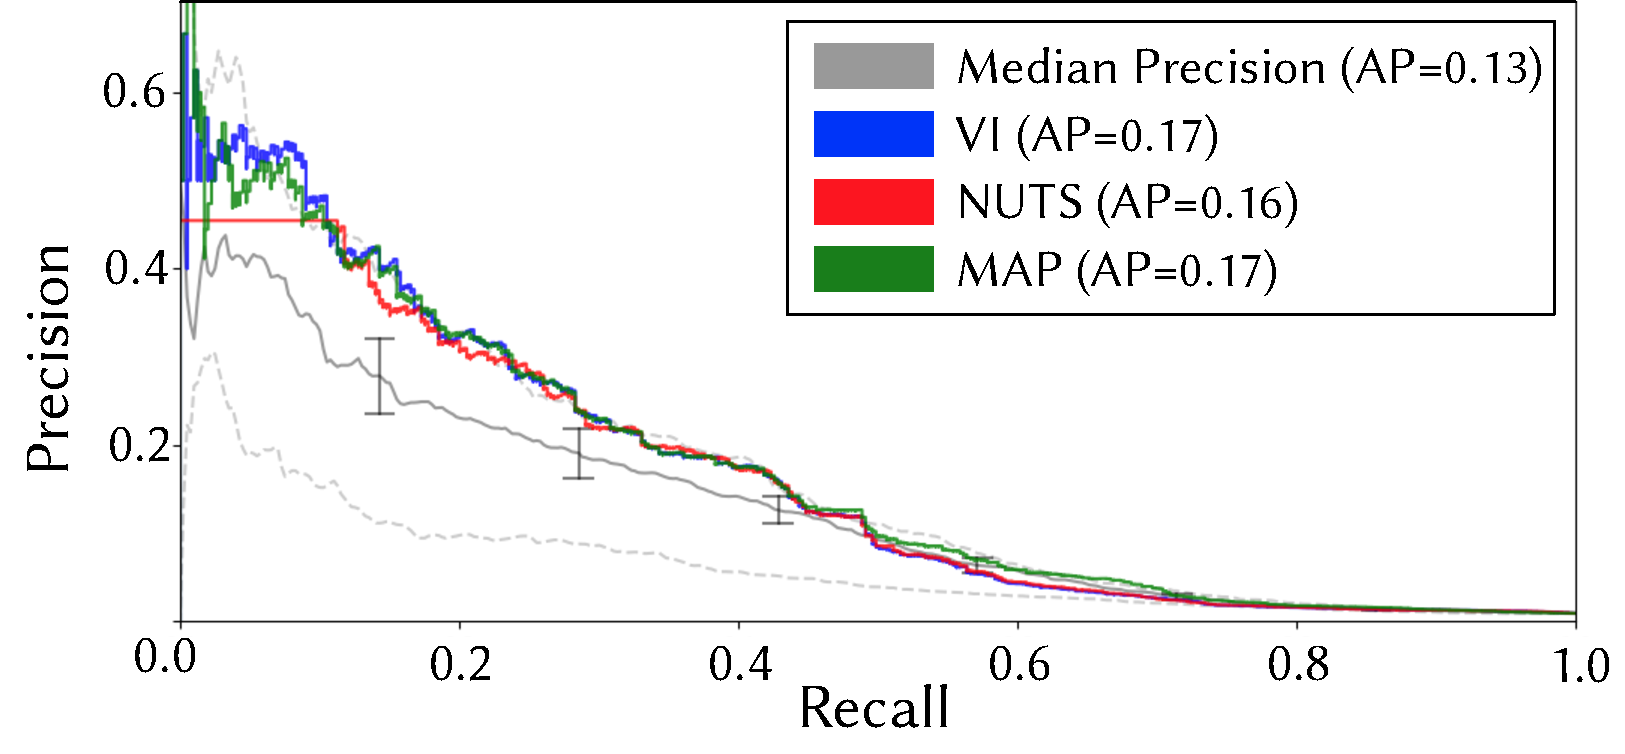
\includegraphics[clip,width=\textwidth]{graphics/chap_04-bayes/fig3_Stage1-single.pdf}
\caption{\footnotesize P/R Curve for iTrust for Stage 1.}
\label{fig:pr1-results}
\end{subfigure}

\begin{subfigure}{0.5\textwidth}
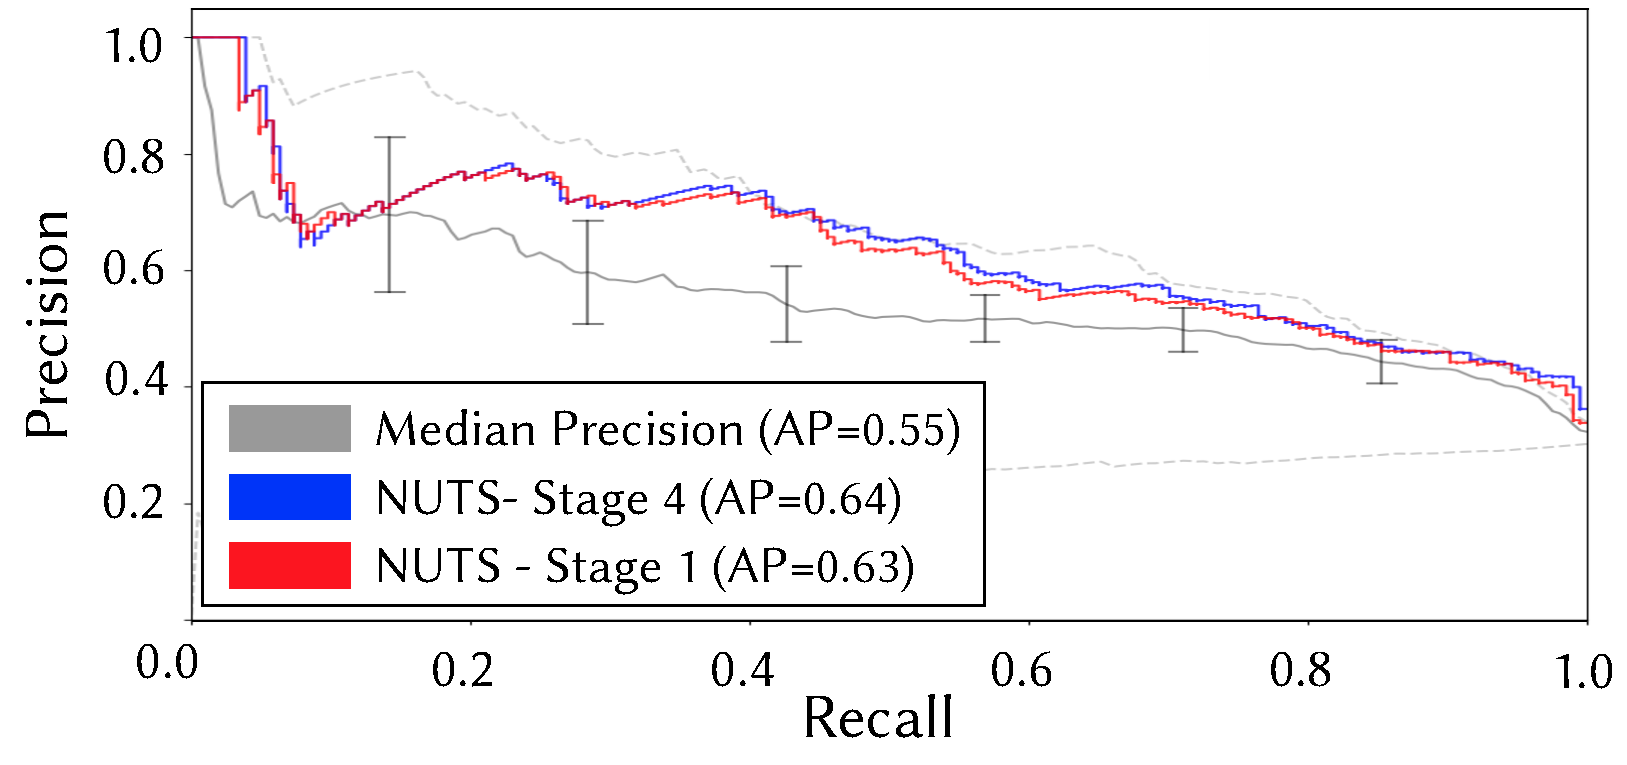
\includegraphics[clip,width=\textwidth]{graphics/chap_04-bayes/fig4_Stage4-single.pdf}
\caption{\footnotesize P/R Curve for I-Net (Req$\rightarrow$Src) for Stage 4.}
\label{fig:pr4-results}
\end{subfigure}

\caption{\footnotesize Selected P/R Curves for Stage 1 and Stage 4 of \Comet.  Solid grey line is median of the baseline IR/ML techniques, dotted grey lines are best and worst performing IR/ML techniques respectively.}

\end{figure}

The AP results for Stage 3 of \Comet, which incorporates transitive relationships between requirements, for both $\tau=0.55$ and $\tau=0.65$ are given in Table \ref{tab:stage3-results} (There were no transitive links in iTrust for $\tau=0.65$). This table also includes the median of the baseline IR/ML techniques, as well as the Comet Stage 1 model AP results, for the set of links affected by transitive relationships (hence the differing Stage 1 columns). The results show that, in general, for $\tau=0.65$ for \Comets Stage 3 model, the accuracy of \Comets inferred trace links improve, with four of the six datasets showing improvements. For $\tau=0.55$ the results generally exhibit similar or slightly worse performance compared to Stage 1.  The fact that the higher value of $\tau$ led to better performance improvements is not surprising, as this parameter essentially controls the \textit{degree of relatedness} required to consider transitive relationships. Thus, a higher value of $\tau$ means that only highly similar transitive requirement relationships are considered by \Comet's model. Using a lower value for this parameter might introduce noise by incorporating transitive relationships between artifacts that don't have as high a degree of similarity. 

The LibEST (Rq$\rightarrow$Src) dataset exhibited decreased performance for $\tau=0.65$, however this is likely because the requirements for this industrial dataset are based on formal format from the Internet Engineering Task Force (IETF). The somewhat repetitive nature of the language used in these requirements could lead to non-related requirements being transitively linked, leading to a decrease in performance. This suggests leveraging transitive relationships between requirements leads to larger performance gains for more unique language. Overall, our results indicate that \Comets Stage 3 model improves the accuracy of links for a majority of subjects.

%------------------------------------------------
\subsection{RQ$_4$ Results: C{\footnotesize OMET} Holistic Performance}
\label{sub:results-rq4}

The AP results for the the holistic \Comet (Stage 4) model are given in Table \ref{tab:stage1-4-results}. These results show that \Comets holistic model outperforms the baseline median IR/ML techniques, and Stage 1 for all subject programs. For three subjects (LibEST Req$\rightarrow$Src, EBT, and iTrust), Comet's holistic model matches or outperforms the best baseline IR/ML technique. \figref{fig:pr4-results} illustrates the P/R curve for the LibEST (Req$\rightarrow$Src) dataset, which shows that the performance gains in inference precision extend for a large range of recall values. The results of these experiments demonstrate that \Comets holistic model is able to effectively combine information from multiple sources to improve its trace link inference accuracy.


%------------------------------------------------
\subsection{RQ$_5$ Results: Industrial Case Study}
\label{sub:results-rq6}

\begin{figure}[h]
\centering
%\vspace{0.2cm}
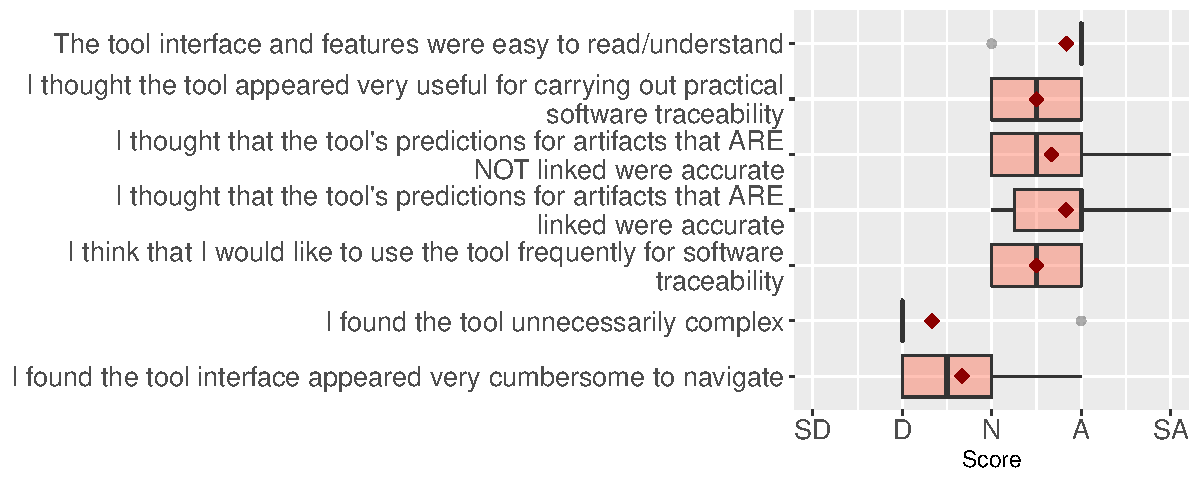
\includegraphics[width=\columnwidth]{graphics/chap_04-bayes/fig5_libest_boxplot.pdf}
%\vspace{-0.7cm}
\caption{Results for LibEST Case Study UX Questions}
%\vspace{-0.0cm}
\label{fig:LibEST-study}
%\vspace{-0.5cm}
\end{figure}

\figref{fig:LibEST-study} provides the responses to the likert-based UX questions from the six developers who work on the LibEST project after interacting with the \Comet plugin. Overall, the responses from these developers were quite positive. They generally agreed the \Comet plugin easy to use and understand, but more importantly, generally found the accuracy of the inferred links and non-links to be accurate. Additionally, we highlight representative responses to the user experience questions in this section, and provide the survey questions with response summaries in our online appendix~\citep{appendix}, in accordance with the NDA established with our industrial partner. Overall the developer responses were encouraging, indicating the practical need for approaches like \Comet. For instance, one developer stated their need for such a tool, \textit{``I really want a tool that could look at test cases and requirements and tell me the coverage. That way the team can know whether we are missing functionality or not.''} Another developer explained the need for a feature that incorporates developer feedback, stating the importance of the \textit{``ability to describe or explain how the code matches up with the code for future reference. Discussion/comments about such explanation as different developers might see links that others don't''}, whereas another developer stated, \textit{``Being able to provide feedback is useful and seeing it update the percentage immediately was nice.''}  This indicates that the support for developer feedback and responsiveness of the \Comet plugin inherently useful. Developers also found the traceability report to be useful, with most criticism suggesting practical UI improvements. For instance, developers appreciated \textit{``The fact that there were the three different options for viewing the traceability between different [artifacts]''}, and \textit{``The ability to bring up the specific requirement quickly in the same window.''}. These responses illustrate the utility that developers saw in the \Comet plugin. Given that these developers had little automated support for traceability tasks, they appreciated any automated assistance. 

We also collected feedback that validated the importance of the practical use cases that the \Comet plugin enabled. In these interviews, the teams generally stated that \Comet would be very useful for code auditing, as one manager stated that it would \textit{``allow compliance analysts to [inspect] links, look at the code and validate [the links]''}. Furthermore, a team responsible for security audits of systems found an interesting use case for \Comet that is often overlooked in traceability analysis. That is, they were interested in code and requirements that are \textit{not linked to any other artifact}, as such artifacts are likely to be suspicious and should be inspected further. In this case, \Comets inferences of non-links would be just as important as the inferences of links. Overall, the interviewed teams saw great promise in \Comet, and expressed interest in adoption.

%------------------------------------------------

\section{Discussion}
\label{sec:discussion-hbn}





%----------------------------------------------------------------------------------------
%	CHAPTER 5: DEEP CODE RETRIEVAL CAUSAL EXPLORATION
%----------------------------------------------------------------------------------------

%\chapter{Causal Discovery}
\label{ch:appI-approach-ii}

%----------------------------------------------------------------------------------------
%	PART II
%----------------------------------------------------------------------------------------

\part{Causality Applications II. Deep Code Interpretability}

%----------------------------------------------------------------------------------------
%	CHAPTER 6: INTERPRETABILITY CONDITIONED
%----------------------------------------------------------------------------------------
\chapter{Understanding Conditioned Neural Code Models}
\label{ch6:conditioned}


%------------------------------------------------

\section{The \codegen Methodology }
\label{sec:approach-conditioned}

This section presents \codegen, a set of causal inference tools to \textit{interpret the prediction performance} of \nlms by connecting causal models to data. \codegen instantiates the concepts and theory discussed in the previous section by introducing three stages (St$_1$-St$_3$): (i) \textit{Modeling Causal Variables}, (ii) \textit{Computing Causal Inference}, and (iii) \textit{Evaluating Causal Effects}. Because \codegen focuses its analysis upon the probability distribution of Next Token Predictions (NTPs) and Cross-Entropy, it falls into the category of model-specific (\ie to \nlms) post-hoc interpretability methods \citep{molnar2019interpret}. We have implemented \codegen in an open source library, which we will make freely available upon acceptance of this paper~\citep{icodegen}.

\subsection{Stage 1 (St$_1$): Modeling Causal Variables}
In this stage, assumptions about relationships among data are defined in a structural causal model similar to Fig.~\ref{fig:scm}, which is later processed in St$_2$ to compute $p(Y|do(T))$. Causal assumptions must be made explicit, which means defining the treatments $T$ (\ie binary: buggy/non-buggy, discrete: layer modifications), potential outcomes $Y$ (\ie global (Cross-Entropy) and local (NTPs) performance), and the common causes $Z$ that can affect the treatments and potential outcomes. For all our SCMs in this study, we assumed that common causes are SE quality metrics since they have the potential to influence models global and local performance, \ie a \nlm may be influenced by more or less for loops, as well as influence treatments, \ie more code has been shown to be correlated with more bugs. In summary, St$_1$ consists of setting down assumptions about the causal relationships of software data employed to interpret \nlms. SCMs help us to describe the relevant features of the software data and how they interact among each other. In the following subsection, we formally define our treatments and potential outcomes.  

\textbf{a. Defining SE Counterfactual Interventions or Treatments.}
\nlms are notorious for not working well outside the distribution they were trained and tested on. For example, if a model trained on a well-commented dataset is applied to predict segments of poorly commented code, this mismatch could potentially impact performance. As such, we assert that observing model performance across datasets with different characteristics can aid in understandability. Hence, we defined \textit{SE Counterfactual Interventions} $T$ to better understand model performance across different settings. We formulate these interventions as testbeds (\ie datasets) organized in sample pairs \textbf{treatment} $T=0$ (\ie BuggyCode) and \textbf{control} $T=1$ (\ie FixedCode). Note that we define testbeds according to different applications often described in SE research. The testbed preparation process is highly dependent on code properties. The general process comprises of identification of some specific \textit{intervention} (\ie program repair) and 2) construction or collection of the necessary data via mining repositories or other means that contain these interventions. More complex interventions will likely be more challenging to prepare. In \codegen, \textit{counterfactual interventions} produce explanations motivated by both semantic perturbations (or treatments) $T_{[data]}$ to our SE Application Settings (\eg Buggy/Fixed, Commented/Uncommented, Clone1/Clone2) and model hyper-parameter variations $T_{[hyp]}$ on \nlms  (\eg layers, units, or heads).

\textbf{b. Defining Potential Outcomes / Model Performance} Cross-Entropy ({Fig.~\ref{fig:performance}-\circled{3}}) and Next Token Prediction ({Fig.~\ref{fig:performance}-\circled{2}}) are relevant values produced at inference time that reflect the effectiveness of a model. By relating these values to counterfactual interventions $T$ (\ie program repair), we can gain an understanding of how well a studied model is \textit{generating code} under these treatments. We refer to Cross-Entropy loss as a measure of a model's \textit{Global Performance} $Y_g: w \to - \sum_{t \in |w|} P(w_t | d_t) \log Q(w_t | w_{<t})$ as these losses capture the overall performance of a \nlm over an entire sequence of tokens $w$. Due to the discrete nature of the data, the expression $P(w_t | w_{t-1:1} )$ can be estimated using a classifier. The classifier, in our particular case, is a \nlm \citep{Bengio2003AModel}. Hence, rather than using \textit{n}-grams or Markov Models to approximate $P(w_t | w_{t-1:1})$ \citep{Karampatsis2020Open-VocabularyAbstract}, it is convenient to use a latent model $P(w_t | w_{t-1:1} ) \approx P(w_t | d_t )$, where $d_t$ is known as a \textit{hidden state} that embeds the sequence information from past observations up to the time step $t$. Depending on \textit{how} the sequence is processed, the hidden state $d_t$ can be computed using either an autoregressive network (\ie such as a Transformer ($TF$)~\citep{vaswani2017transformers}) or a Recurrent Neural Network ($RNN$). Conversely, Next Token Prediction (NTP) values signal \textit{Local Performance} $Y_l:w_{<t} \to P(w_t | w_{t-1:1})$ within token-level contexts. NTPs capture local predictions for individual tokens that are affected by complex interactions in \nlms and are equivalent to the estimated predicted value (or softmax probability) $\sigma(k)_t$ for each token. Bear in mind that the size of the vector $\sigma(k)_t$ is the vocabulary $|\mathcal{V}|$, in which $k$ represents the non-normalized log probabilities for each output token $t$. NTPs capture the value of the expected token $w_t$ instead of the maximum value estimated in the vector $\sigma(k)_t$.

\begin{figure}[h]
		\centering
		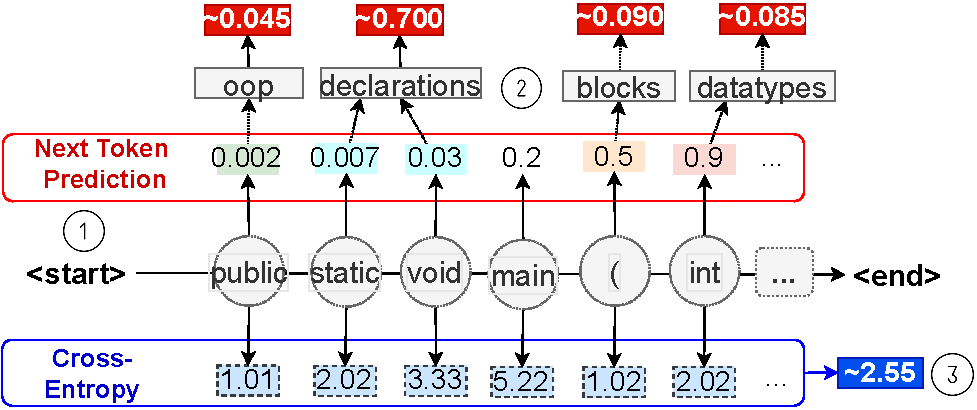
\includegraphics[width=0.9\textwidth]{graphics/preliminaries/fig_2_performance.pdf}
		%\vspace{-0.3cm}
		\caption{Potential Outcomes are Prediction Performance of  \nlms: Cross-Entropy $(Y_g)$ and Next Token Predictions $(Y_l)$.}
        %\vspace{-0.1cm}
        \label{fig:performance}
\end{figure}

A major conjecture in interpretability research is that \nlms are more understandable when they \textit{reflect human knowledge} \citep{Kim2018InterpretabilityTCAV}. One way of determining whether a model reflects human knowledge is testing it to see whether or not it operates (or predicts) \textit{similar to how a human would operate}. \codegen accomplishes this by mapping the complex interactions present in both Global $Y_g$ and Local $Y_l$ Potential Outcomes of a \nlm to human interpretable PL features and testbeds. Below we provide a motivating example for this mapping function, which we formally introduce in Definition \ref{def:taxonomy}:

\begin{exmp}
\label{exmp:outcome}
Consider the situation where a developer inserts a \texttt{\small `('} character after the \texttt{\small `main'} keyword in a function declaration in Java ({\circled{1}}-Fig.~\ref{fig:performance}). Inherently, a developer mentally rationalizes several things such as the concept of a function declaration and expected Java syntax. If a \nlm is able to make a similar prediction, it suggests to us that it has \textit{statistically learned} some understanding of the concept of a function declaration and corresponding syntax. Thus, we assert that by ascribing human-interpretable properties, and in particular code-related properties, to model predictions, and then analyzing the statistical properties of those predictions, we can begin to learn how well a given \nlm reflects human knowledge. We propose a \textit{Structural Code Taxonomy} $\mathcal{H}$ to bridge this interpretability gap.
\end{exmp}

\marginnote{
    \begin{definition}
    \label{def:taxonomy}
    \textbf{Structural Code Taxonomy.} In programming languages (PL), different types of tokens retain different semantic meanings. For instance \texttt{\small `='} and \texttt{\small `<'} are common \operators. As such, we can group tokens into semantically meaningful \textit{categories}. Fig.~\ref{fig:taxonomy} depicts an initial version of \codegen's taxonomy derived from Java. These features will allow \codegen to assign semantic meaning to predicted tokens $\hat{w_t}$. The taxonomy comprises high-level properties of code using a \textbf{mapping function} $\phi_{\mathcal{H}}: \vec{w} \to \vec{h} $, where the vector $\vec{w}$ corresponds to tokens of the vocabulary $\mathcal{V}$. Each token in a sequence $w$ is assigned to a taxonomy category $h \in \mathcal{H}$.
    \end{definition}
}

With our categories $\mathcal{H}$, researchers and practitioners can easily associate \nlm performance (\ie $Y_g$ or $Y_l$) to particular structural code attributes. As such, by using our structural code taxonomy, \codegen allows for \nlm predictions to be interpreted in a developer-centric way. These categories represent a “base” case as the keywords of any PL can likely be grouped into interpretable categories. This is why anyone using \codegen can \textit{easily define their own mapping function} $\phi_{\mathcal{H}}$ (\eg using coupling and cohesion metrics), and stipulate them in a JSON-like configuration file. For instance, a researcher working to analyze how well \nlms learn to predict cryptographic APIs could define a taxonomy based upon “safe” and “unsafe” APIs.

 \begin{marginfigure}
		\centering
		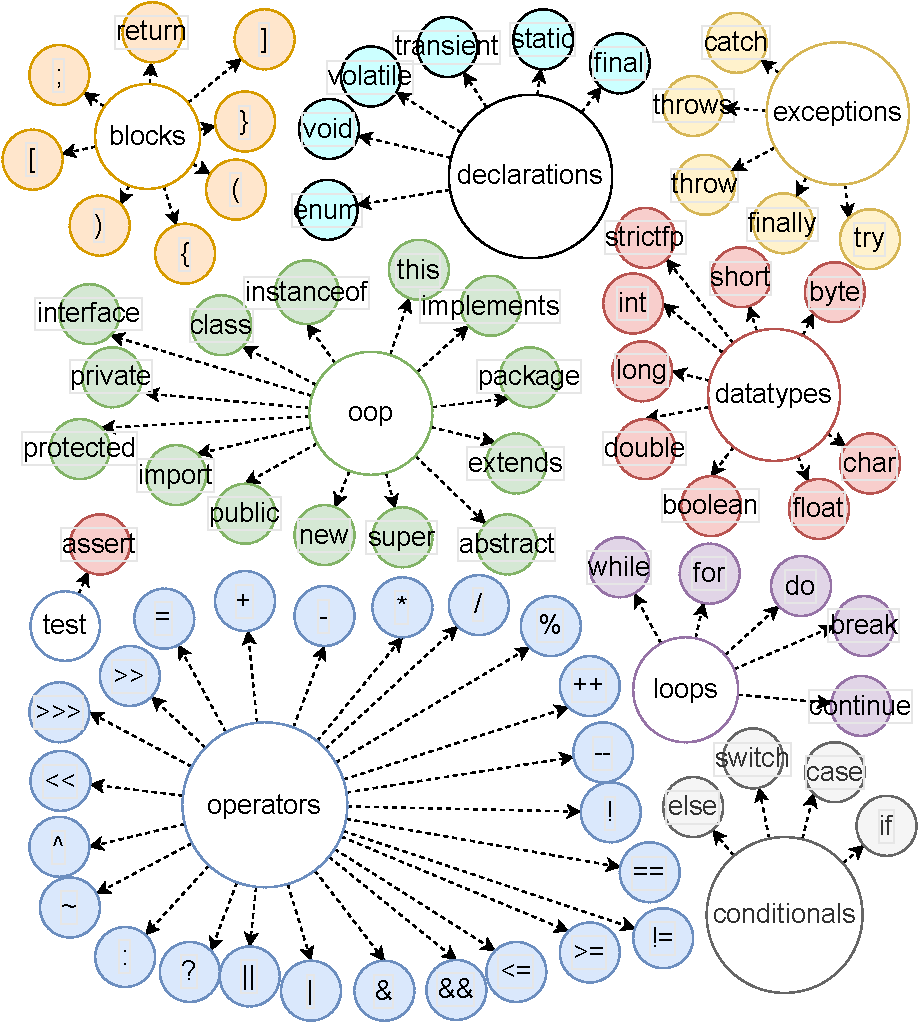
\includegraphics[width=\textwidth]{graphics/preliminaries/fig_3_taxonomy.pdf}
		\caption{Structural Code Taxonomy $\mathcal{H}$ for Java}
        \label{fig:taxonomy}
\end{marginfigure}

\subsection{Stage 2 (St$_2$): Computing Causal Inference (CI)}
%Definition of Causal Inference
According to Pearl \& Mackenzie \citep{Pearl2018Causality}, CI seeks answers to questions of association (\textit{what is?}), counterfactual interventions (\textit{what if?}), and pure counterfactuals (\textit{why?}). The authors introduce the concept of \textit{levels of causation} to match distinct levels of cognitive ability with concrete actions: seeing~(\textit{level 1}), doing~(\textit{level 2}), and imagining~(\textit{level 3}). Our proposed analysis is primarily concerned with levels 1 \& 2. Level 1 causation, namely association, $p(Y|T)$ is estimated by using typical correlation methods (\eg Pearson, Spearman, or Covariance) in addition to functional associations such as $y=g(t)$, which can be predicted with regressions or ML methods. For binary treatments similar to the ones we used in $T_{[data]}$ (\eg Buggy/Fixed, Commented/Uncommented, Clone1/Clone2), we opt to employ Pearson correlations and Jensen-Shannon distance as association estimand for level 1 causation. We will now formally define each of these below \david{Contextualize the functions below}.

\marginnote{
\begin{definition}
\label{def:js}
\textbf{Jensen-Shannon Distance (JS).} The Jensen-Shannon divergence (JSD) overcomes the asymmetric computation of the KL divergence and provides a measure of difference between distributions Eq.~\ref{eq:js_divergence}. The JS distance is the square of the JS divergence $p(Y|T)\approx JS(Y^{T=0},Y^{T=1}) = JSD(Y^{0},Y^{1})^2$. JS is proportional to the influence of $T$ on $Y$, which measure the separation of the distributions $Y^{0},Y^{1}$. The notation $Y^{T=0}$ refers to the potential outcomes observed under the treatment $T=0$. 

\end{definition}
}

\begin{subequations}
    {%\tiny %footnotesize
    \begin{align}
     JSD(Y^{0}=y^0,Y^{1}=y^1) &&= \label{eq:js_divergence-1}\\
     \frac{1}{2}\left[ D_{KL}\left(y^0||\frac{y^0+y^1}{2}\right) + D_{KL}\left(y^1||\frac{y^0+y^1}{2}\right)\right] &&= \label{eq:js_divergence-2}
    \end{align}
    }
\label{eq:js_divergence}
\end{subequations} 

\begin{exmp}
\label{exmp:js}Imagine we wish to understand the correlation between syntactic changes, \ie variable renaming, alterations in white space, \etc and a \nlms performance. One way we can study this is through computing the association of Cross-Entropy values $Y$ under two treatments, the first $T=0$, would be an unaltered code snippet and the second $T=1$ would be its Type III clone. Computing this association can be done using the JS distance $p(Y|T)\approx JS(Y^0,Y^1)$ as defined in Def.~\ref{def:js} for four models. Fig.~\ref{fig:jssimilarity} shows the distributions of $Y^0$ and $Y^1$ with their distances after applying bootstrapping as an example.

\begin{figure}[th]
  \centering
  \begin{subfigure}[b]{0.46\linewidth}
    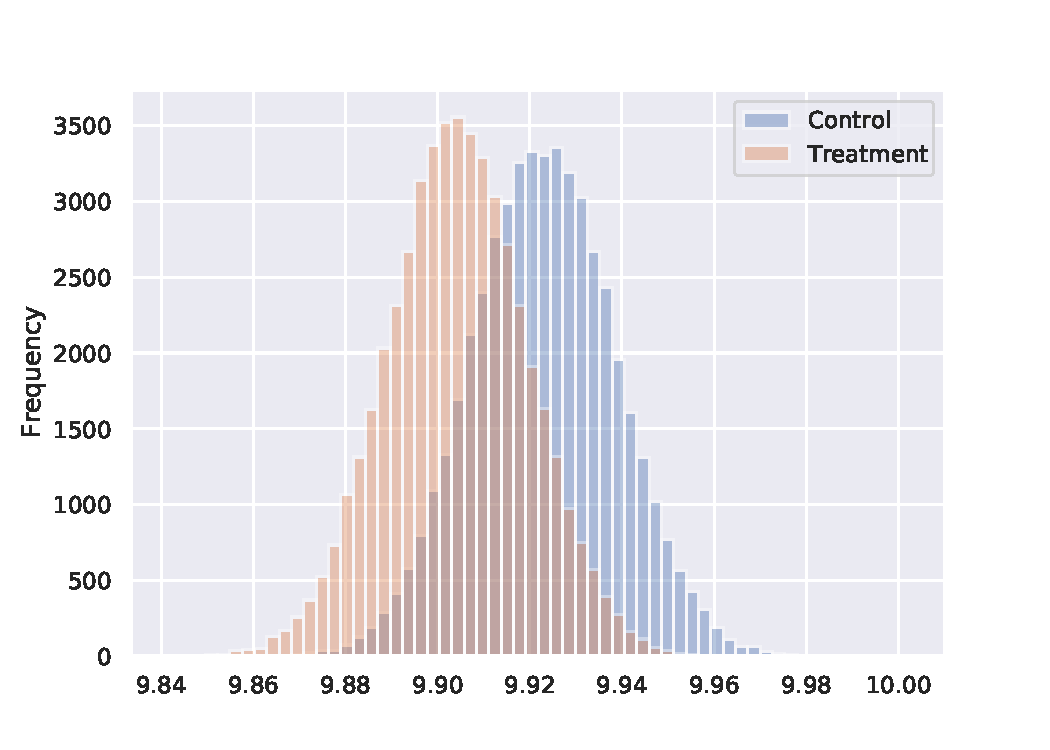
\includegraphics[width=\linewidth]{graphics/preliminaries/association/cross-entropy-rnn1-distribution-clone3-300dpi.pdf}
    %  \caption{RNN1.}
  \end{subfigure}
  \begin{subfigure}[b]{0.46\linewidth}
    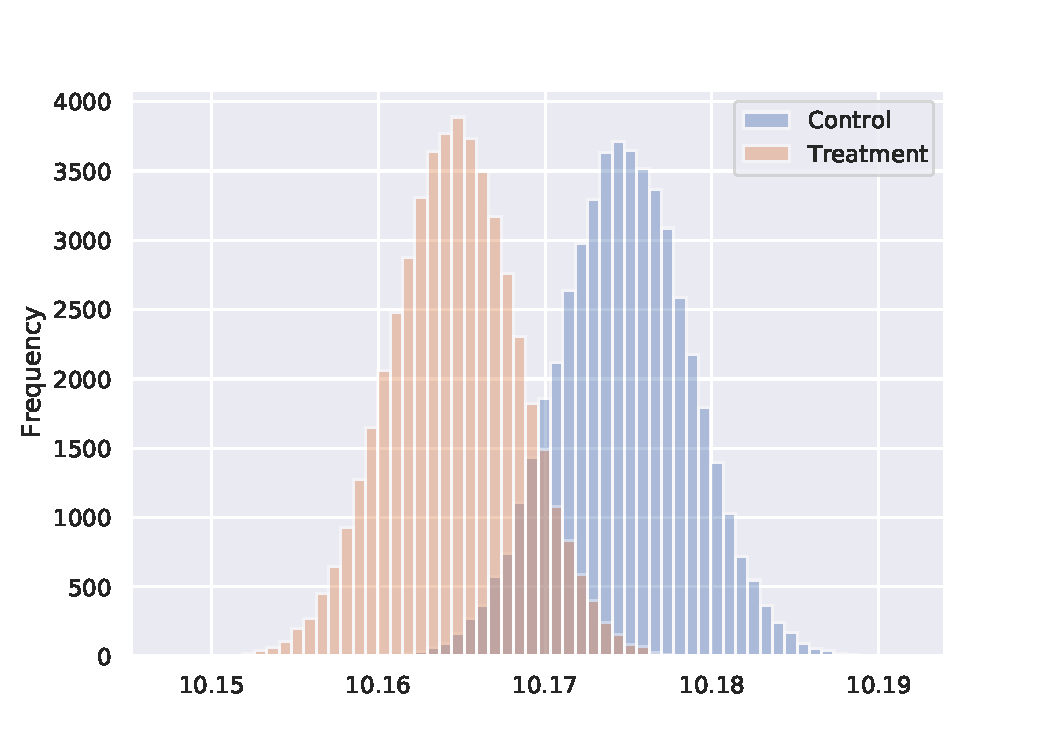
\includegraphics[width=\linewidth]{graphics/preliminaries/association/cross-entropy-gru1-distribution-clone3-300dpi.pdf}
    % \caption{GRU1.}
    % \vspace{0.2cm}
  \end{subfigure}
  \begin{subfigure}[b]{0.46\linewidth}
    % \vspace{-0.2cm}
    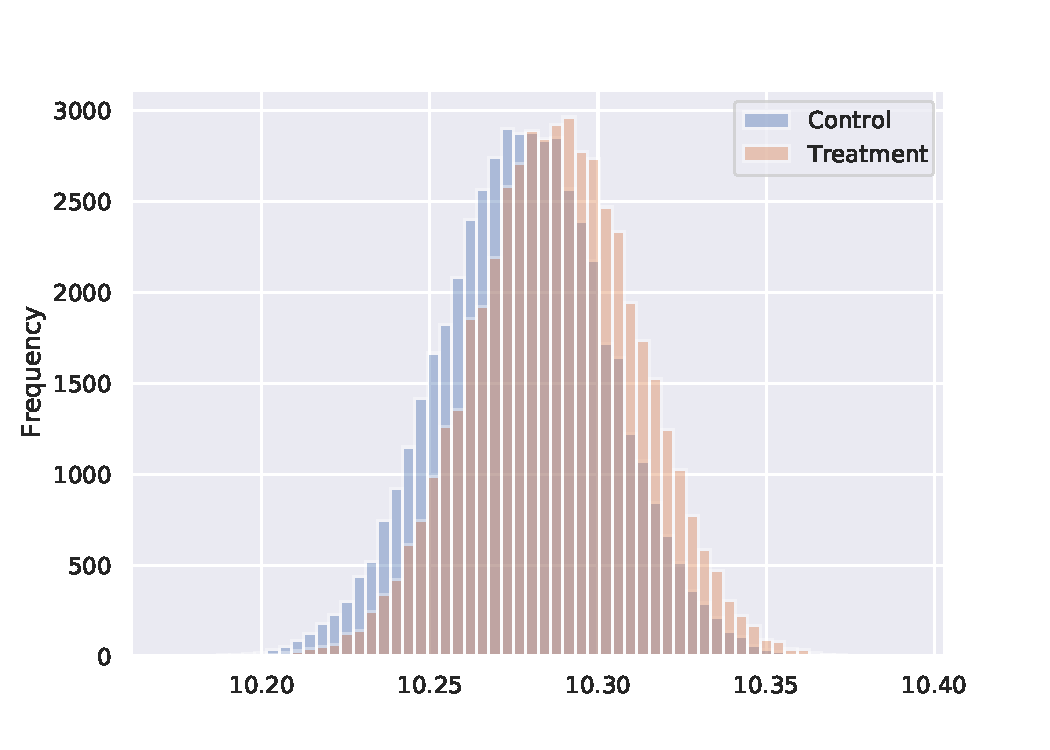
\includegraphics[width=\linewidth]{graphics/preliminaries/association/cross-entropy-tf1-distribution-clone3-300dpi.pdf}
    % \caption{TF1.}
  \end{subfigure}
  \begin{subfigure}[b]{0.46\linewidth}
    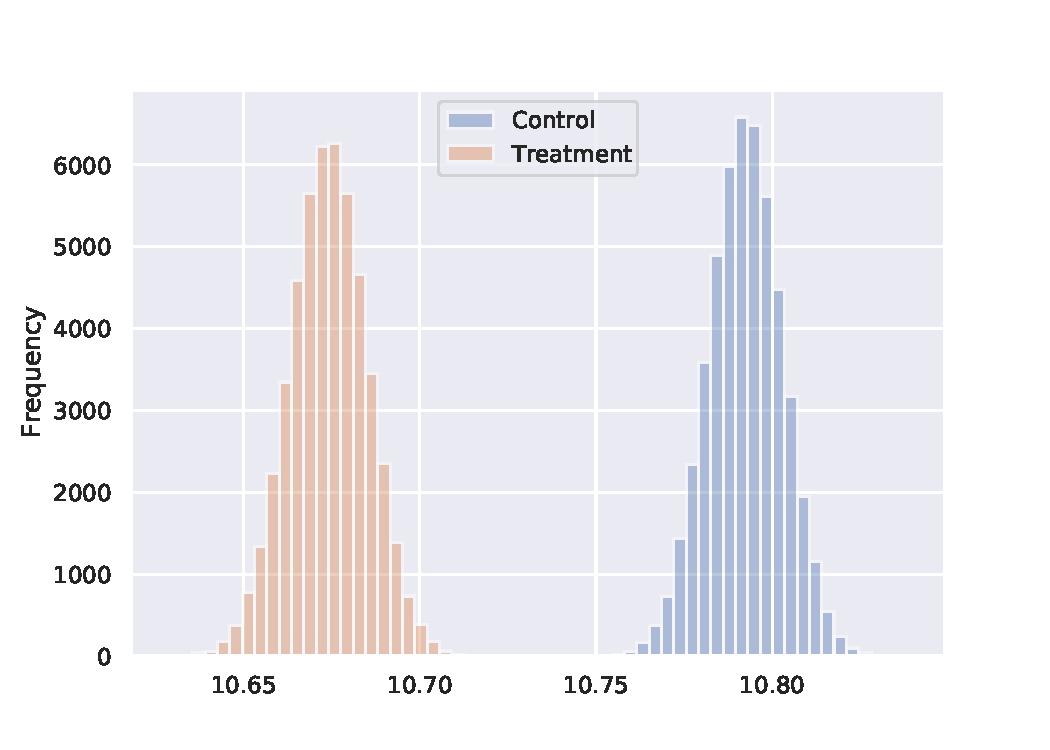
\includegraphics[width=\linewidth]{graphics/preliminaries/association/cross-entropy-tf2-distribution-clone3-300dpi.pdf}
    % \caption{TF2.}
  \end{subfigure}
  \vspace{-0.2cm}
  \caption{\datainterII Intervention (\BigCloneIIITB) for Global Performance: Bootstrapped Cross-Entropy. Top Left: \rnn ($JS=0.3$), Top Right: \gru ($JS=0.8$), Bot Left: \tf ($JS=0.6$), Bot Right: \tfi ($JS=1$).}
  \label{fig:jssimilarity}
  \vspace{-0.3cm}
\end{figure}

\end{exmp}

Now, if we want to go beyond \textit{``what is''} type questions, we must move past simple correlations and association. This requires the $do-operator$ found in level 2, causation $p(y|do(t))$. Specifically, it is estimated for a population (\ie SE dataset) by computing an \textit{Average Treatment Effect} based on the Def.~\ref{def:effect} introduced in Sec.~\ref{sec:pre-ci4se}.

\marginnote{
\begin{definition}
\label{def:ate}
\textbf{Average Treatment Effect (ATE)} Defining the first intervention as $do(T=1)$ and the second by $do(T=0)$, the Average Treatment Effect is the population average of the difference of causal effects of each code snippet $x$.  
\end{definition}
}

\david{Contextualize the functions below}
\begin{subequations}
    \begin{align}
     ATE = \mathbb{E}_{x\sim p(x)}[Y=y|x,do(T=t)]  &= \label{eq:ate-1}\\
     \mathbb{E}_{x\sim p(x)}[ \mathbb{E}[Y|x,do(T=1)] - \mathbb{E}[Y|x,do(T=0)] ] &= \label{eq:ate-2}\\
     \mathbb{E}_{x\sim p(x)}[ \mathbb{E}[Y^{1}|x,T=1] - \mathbb{E}[Y^{0}|x,T=0] ] &= \label{eq:ate-3}
    \end{align}
\label{eq:ate}
\end{subequations} 


ATE can be computed in two steps as follows:

\textbf{a. Identifying Causal Effects.} Once the SCM (similar to Fig.~\ref{fig:scm}) is constructed, \codegen applies various techniques (\ie backdoor-criterion and instrumental variables) to determine the adjustment formula Eq.~\ref{eq:effect}, which will control for confounding common causes when computed. For our case study, the causal effect $p(Y|do(T))$ is computed, which will be done in the next step, based on the following causal graph: data-based $T_{[data]}$ and parameter-based $T_{[hyp]}$ treatments; SE covariates $Z \in SE_{metrics}$; and potential outcomes $Y_l, Y_g$.

\textbf{b. Estimating Causal Effects.} Next, \codegen estimates the causal effect using statistical and ML methods based on the adjustment formula from the previous step. \codegen computes \textit{Propensity Score Matching} for binary SE treatments (\ie Buggy/Fixed) and \textit{Linear Regressions} for SE discrete treatments (\eg layers, units, or heads). We refer interested readers to the \textit{doWhy} documentation for the full process details \citep{dowhy}. For completeness, we will now show how to estimate a causal effect assuming a binary treatment as an example. Eq.~\ref{eq:ate} shows the formal definition of an \textit{ATE}. We can derive the final expression by applying the law of total expectations and the ignorability assumption  $Y \perp\!\!\!\perp  Z|T$, where the potential outcomes $Y$ are independent of treatment assignments conditioned on covariates $Z$ \citep{Pearl2009Causality}. That is, the effects of the hidden common causes $Z$ and missing data are ignored. In Eq.~\ref{eq:ate}, the term $\mathbb{E}[Y^1|x,T=1]$ represents the expected value of a potential outcome under an observable treatment (\ie FixedCode). Similarly, the term $\mathbb{E}[Y^0|x,T=0]$ represents an expected value of a potential outcome under an observable control (\ie BuggyCode). Both terms are quantities that can be \textit{estimated from data}. Covariate adjustment (in Eq.~\ref{eqn:do-all-lines}), propensity score (in Eq.~\ref{eq:effect-3}), and linear regression are some of the estimation methods that we employ to estimate the $ATE$. Their usage depends upon the type of the treatment variable (\ie binary, discrete, or continuous) and causal graph assumptions.

\subsection{Stage 3 (St$_3$): Evaluating Causal Effects}
The previous causal estimation can be validated using \textit{refutation methods} that calculate the robustness of the causal estimate. In essence, the refutation methods apply random perturbations to the original causal graph to test for robustness of the estimated $ATE$. We chose four methods for our analysis: Adding a random common cause or covariate $\mathcal{R}_1$, adding an \textit{unobserved} common cause or covariate $\mathcal{R}_2$, replacing the treatment with a random variable or placebo $\mathcal{R}_3$, and removing a random subset of the data $\mathcal{R}_4$. For robustness, we expected that $\mathcal{R}_1$, $\mathcal{R}_2$, and $\mathcal{R}_4$ values were close to the $ATE$ (Eq.~\ref{eq:ate}). Conversely, the placebo $\mathcal{R}_3$ should tend to zero.

In addition to measuring refutation methods, it is relevant to identify cases of \textit{spurious correlations} (\ie \textit{Confounding Bias}) or cases where $p(Y|T)\neq p(Y|do(T))$. Typically, association is not causation due to the influence of a common cause or confounding variable $Z$. Such a variable is the one that is being controlled for or adjusted by means of Eq.~\ref{eqn:do-all-lines}. Nonetheless, we can still compute the correlation $d(Y|Z)$ to assess the variables that are actually affecting potential outcomes. 

 \begin{marginfigure}
		\centering
		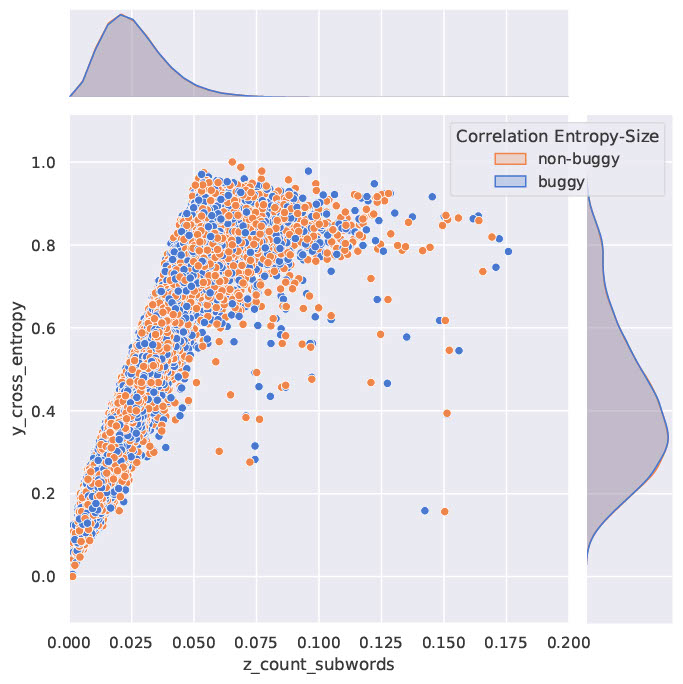
\includegraphics[width=\textwidth]{graphics/fig_4_covariates_corr.jpg}
		\caption{ \textit{Spurious Correlation} between the \textit{Number of Subwords} common cause and Cross-Entropy values ($p(Y|Z)\approx0.87$) for the \datainterI intervention generated from \tf. } 
        %\vspace{-0.5cm}
        \label{fig:covariate}
\end{marginfigure}

\begin{exmp}
\label{exmp:confounding}

Consider the \datainterI intervention where $T$ is Buggy/Fixed code, $Y$ is the cross-entropy of each of method of the dataset \BuggyTB, and $Z$ is the \textit{Number of Subwords} for each method. There exists a spurious correlation after calculating JS and ATE, $p(Y|T)\approx0.67$ and $p(Y|do(T))\approx-0.0002$. One possible explanation is that the common cause $Z$ is confounding the relationship between the treatment and the outcome. Fig.~\ref{fig:covariate} depicts the influence of $Z$ on the potential outcome $Y$ for BuggyCode ($p(Y|Z,T=Buggy)\approx0.87$) and FixedCode ($p(Y|Z,T=Fixed)\approx0.86$). Blue and orange points in the plot are code snippets from the dataset. These points are equally distributed, which suggest that the \datainterI intervention has a negligible impact on the Cross Entropy. 
\end{exmp}

%------------------------------------------------

\section{Case Study Design in Code Generation}
\label{sec:design-conditioned}

%Intro
In order to illustrate the insights that \codegen can enable, we present a case study that serves as a practical application of our interpretability method by analyzing two popular \nlms: RNNs and Transformers. In this section, we detail the methodological steps we took to configure our models and process our datasets. In addition, we designed our methodology for causal understanding following Pearl~\etal's guidelines \citep{Pearl2016Causality,Sharma2021DoWhyAssumptions}. We adopted these guidelines to formulate two research questions: \ref{rq:causal} SE Intervention Effects and \ref{rq:eval} Stability Causation.

\begin{enumerate}[label=\textbf{RQ$_{\arabic*}$:}, ref=\textbf{RQ$_{\arabic*}$}, wide, labelindent=5pt]\setlength{\itemsep}{0.2em}
      \item \label{rq:causal} {\textit{To what extent do SE data and model interventions affect code prediction performance?}} 
       \begin{enumerate}[label=\textbf{RQ$_{1.\arabic*}$:}, ref=\textbf{RQ$_{1.\arabic*}$}, wide, leftmargin=0.5cm]\setlength{\itemsep}{0.2em}
        \item \label{rq:global}{\textit{What is the influence of our interventions on global performance?}}
        \item \label{rq:local}{\textit{What is the influence of our interventions on local performance?}}
        \end{enumerate}
      \item \label{rq:eval} {\textit{How robust are the treatment effects based on SE interventions?}}
\end{enumerate}

\begin{table*}[b]
\centering
\caption{Counterfactual Interventions Case Study. NLMs include Recurrent Nets (GRUs) and Transformers (TFs). 
%The units of TFs are heads [hds]. 
}
\vspace{0.2cm}
\label{tab:method}

%\scalebox{0.65}{%
\resizebox{\textwidth}{!}{
%%%%%%%%%%%%%%%%%

\begin{tabular}{@{}llllll|llll@{}}
\toprule
\multicolumn{6}{c|}{\textbf{Case Study Methodology}} &
  \multicolumn{4}{c}{\textbf{\nlms Training}} \\ \midrule
\multicolumn{4}{c}{\textit{\textbf{\begin{tabular}[c]{@{}c@{}}Counterfactual\\ Interventions\end{tabular}}}} &
  \multicolumn{2}{c|}{\textit{\textbf{\begin{tabular}[c]{@{}c@{}}Proposed Experiments\\ Global and Local\end{tabular}}}} &
  \multicolumn{1}{c}{\textit{\textbf{RNNs}}} &
  \multicolumn{1}{c|}{\textit{\textbf{Transformers}}} &
  \multicolumn{1}{c}{\textit{\textbf{Hyper.}}} &
  \multicolumn{1}{c}{\textit{\textbf{Val.}}} \\ \midrule
\multicolumn{1}{c}{\textit{Type}} &
  \multicolumn{1}{c}{\textit{Interv.}} &
  \multicolumn{1}{c}{\textit{Case}} &
  \multicolumn{1}{c}{\textit{Associated Dataset}} &
  \multicolumn{1}{c}{\textit{Avg. Causation}} &
  \multicolumn{1}{c|}{\textit{Correlation}} &
  \textit{\nlm $_{lyr,unt}$} &
  \multicolumn{1}{l|}{\textit{\nlm$_{lyr,hds}$}} &
  \multirow{6}{*}{\begin{tabular}[c]{@{}l@{}}dropout RNN\citep{Karampatsis2020BigCode}\\ dropout TF\\ optimizer\citep{Kingma2015AdamAM}\\ learning rate\\ beta1$|$beta2\\ epsilon\\ epochs\\ batch RNN$|$TG\end{tabular}} &
  \multirow{6}{*}{\begin{tabular}[c]{@{}l@{}}0.5\\ 0.l\\ adam\\ 1e-3\\ 0.9\\ 1e-7\\ 64\\ 512$|$128\end{tabular}} \\ \cmidrule(r){1-8}
\multirow{3}{*}{\textit{Data}} &
  $T_{dat0}$ &
  \datainterI &
  \BuggyTB\citep{Tufano2019LearningBug-Fixes} &
  \colorbox{blue!10}{$p(Y_{g,l}|do(T_{dat0}))$} &
  \colorbox{blue!10}{$p(Y_{g,l}|T_{dat0})$} &
  \multirow{5}{*}{\begin{tabular}[c]{@{}l@{}}\rnn\\ \gru\\ \grui\\ \gruii\\ \gruiii\\ \gruiv\end{tabular}} &
  \multicolumn{1}{l|}{\multirow{5}{*}{\begin{tabular}[c]{@{}l@{}}\tf\\ \tfi\\ \tfii\end{tabular}}} &
   &
   \\
 &
  $T_{dat1}$ &
  \datainterIII &
  \CommentsTB\citep{husain2019codesearchnet} &
  \colorbox{blue!10}{$p(Y_{g,l}|do(T_{dat1}))$} &
  \colorbox{blue!10}{$p(Y_{g,l}|T_{dat1})$} &
   &
  \multicolumn{1}{l|}{} &
   &
   \\
 &
  $T_{dat2}$ &
  \datainterII &
  \begin{tabular}[c]{@{}l@{}}\BigCloneIITB\citep{Svajlenko2015EvaluatingBigCloneBench}\\ \BigCloneIIITB\citep{Svajlenko2015EvaluatingBigCloneBench}\end{tabular} &
  \colorbox{blue!10}{$p(Y_{g,l}|do(T_{dat2}))$} &
  \colorbox{blue!10}{$p(Y_{g,l}|T_{dat2})$} &
   &
  \multicolumn{1}{l|}{} &
   &
   \\ \cmidrule(r){1-6}
\multirow{2}{*}{\textit{Model}} &
  $T_{hyp0}$ &
  \modelinterI &
  \multirow{2}{*}{\training\citep{husain2019codesearchnet}} &
  \colorbox{blue!10}{$p(Y_{g,l}|do(T_{hyp0}))$} &
  \colorbox{blue!10}{$p(Y_{g,l}|T_{hyp0})$} &
   &
  \multicolumn{1}{l|}{} &
   &
   \\
 &
  $T_{hyp1}$ &
  \modelinterII &
   &
  \colorbox{blue!10}{$p(Y_{g,l}|do(T_{hyp1}))$} &
  \colorbox{blue!10}{$p(Y_{g,l}|T_{hyp1})$} &
   &
  \multicolumn{1}{l|}{} &
   &
   \\ \bottomrule
\end{tabular}


%%%%%%%%%%%%%%%%%%


}
\vspace{-0.35cm}

\end{table*} 

\codegen adapts causal inference theory to aid in providing explanations for both global $Y_g$ (\ref{rq:global}) and local $Y_l$ (\ref{rq:local}) prediction performance of given \nlms. Before \codegen can be performed, a researcher or practitioner making use of our method must select the \nlms and define \textit{hyper-parameter variations} $T_{[hyp]}$ and \textit{data perturbations} $T_{[data]}$ that they would like to examine in Stage 1 ($St_1$). Here, \textit{hyper-parameter variations} are essentially different configurations of a given model according to attributes such as capacity (layers) or the types of layers. Additionally, the researcher must define their code \textit{testbeds}. \codegen offers the possibility of adding additional testbeds with data \textit{perturbations} that represent a set of SE-based interventions or Application Settings. After defining and estimating the causal effect (\ref{rq:causal}) of proposed interventions in Stage 2 ($St_2$), \codegen helps to evaluate the robustness of ATE's results by performing refutation methods proposed in Stage 3 ($St_3$) (\ref{rq:eval}).

\subsection{Context: Data Processing \& Model Training}
To train our \nlms we made use of the Java portion of the commonly used \training Challenge dataset~\citep{husain2019codesearchnet}, which consists of a diverse set of methods (mts) from GitHub \citep{github}. \training is split into a training, validation, and test set. For the testbeds for interpreting the performance of our \nlms using \codegen, we collected four datasets from the \textit{CodeXGLUE} project that contain control and treatment groups \citep{DBLP:journals/corr/abs-2102-04664}. Tab.~\ref{tab:method} shows the generated testbeds containing parallel corpora for understanding the impact of buggy code (\BuggyTB: 64,722 mts), the impact of code documentation (\CommentsTB: 6,664 mts), and syntactic alterations on semantically equivalent snippets based on type II (\BigCloneIITB: 666 mts) and type III (\BigCloneIIITB: 8,097 mts) clones from \BigCloneTB. The only additional filtering we performed on the training, validation, and testbeds was the removal of methods that contain any non-ASCII characters and, for the \CommentsTB, removal of methods that do not have comments.  We derived the uncommented portion of the \CommentsTB by removing any existing comments from the Java test set of the \training dataset.

We performed Byte Pair Encoding (BPE) tokenization \citep{sennrich2015neural} across all testbeds before they were processed by our studied \nlms. BPE has shown to be extremely beneficial for training \nlms on code to overcome the \textit{out-of-vocabulary} problem \citep{Karampatsis2020BigCode}. We trained a BPE tokenizer on 10\% of our training data and used a vocabulary size of 10K. Due to the tokenization process of BPE, some subtokens contained multiple reserved keywords or characters if they appeared frequently together. This was problematic for our interpretability analysis since the function $\phi_{\mathcal{H}}$ relies on the ability to map model predictions to our structural taxonomy. Having certain reserved keywords and tokens merged into BPE subtokens would make it impossible for us to perform this mapping. Therefore, we fixed all reserved keywords and tokens (Fig.~\ref{fig:taxonomy}) to be detected by our trained BPE model.

As for the model training, we used Tensorflow and Pytorch \citep{tensorflow2015-whitepaper, pytorch} (Huggingface's Transformers library \citep{wolf2020transformers}) for creating and training our different models. Our $RNN$ and $TF$ models were trained on \training Java training set. All models reached optimal capacity as they all early terminated to prevent overfitting, with a patience of $5$ epochs without improvement on cross-entropy of at least $1\text{e-2}$. Additionally, we added a \textit{start of sentence} token to the beginning of the input, padded and truncated all inputs to $300$. The training was executed on a 20.04 Ubuntu with an AMD EPYC 7532 32-Core CPU, A100 NVIDA GPU with 40GB VRAM, and 1TB RAM.

\subsection{Case Study Methodology}
We provide an overview of our case study summarized in Tab.~\ref{tab:method}, which follows the \codegen methodology introduced in Sec.~\ref{sec:appII-approach}. This section provides the details regarding how we instantiated \codegen's methodology for our studied models and testbeds. On one hand, we empirically estimated $p(Y|T)$ using two methods: Pearson correlations and Jensen-Shannon Similarities (explained in Def.~\ref{def:js}). On the other hand, we estimated $p(Y|do(T))$ using the \textit{doWhy} library \citep{Sharma2021DoWhyAssumptions} and ATE (explained in Def.~\ref{def:ate}).

\codegen is extensible and researchers can define their own treatments. In our case study, we suggested three \textit{data interventions} $T_{[data]}$ (see row \textit{Data} in Tab.~\ref{tab:method}). In addition, the aim of the syntax analysis was to determine how robust \nlms are in the presence of minor and major syntactic variations of semantically equivalent code snippets. That is, we assessed how semantic preserving changes affect code generation. Since there is no natural split for the different clone types, we were unable to perform a causal analysis on the \BigCloneTB dataset using the typical control and treatment settings. This is because the choice of one clone compared to another is arbitrary when evaluating the set of what \BigCloneTB calls \textit{function$_1$} and \textit{function$_2$} methods. Therefore, instead of our standard covariates, we used the differences between \textit{function$_1$} and \textit{function$_2$} of the different clone types. Specifically, we used the Levenshtein Distance $T_{[dat1]}$, a measure of the difference between two sequences in terms of the necessary edit operations (insert, modify, and remove) needed to convert one sequence into the other, to approximate a treatment where one method was \textit{refactored} into another method by a specific number of edit operations. This formulation allowed us to avoid needing a natural split between \textit{function$_1$} and \textit{function$_2$} and focused on how syntactic differences of methods that perform the same function, \ie semantically similar, affects our models. 

As for the \textit{model interventions} $T_{[hyp]}$ (see row \textit{Model} in Tab.~\ref{tab:method}), our case study consists of an investigation of two different \nlm architectures. We also investigated how layer and unit variations in each architecture affect their performance. We made use of two different types of RNN architectures, a ``base'' model and a model that includes Gated Recurrent Units (GRU). Additionally, we studied a GPT-based Transformer model~\citep{Cho2014GRU, Radford2018ImprovingLU} for our autoregressive model. We chose these two models because RNNs have been extremely popular in SE \citep{watson2020dl4se} and Transformers have recently gained popularity due to the high performance they have achieved in the NLP domain~\citep{Mastropaolo2021StudyingTasks}.

%------------------------------------------------

\section{Results and Discussion}
\label{sec:results}

\subsection{\ref{rq:global} SE Intervention on Global Performance}

% Please add the following required packages to your document preamble:
% \usepackage{multirow}
\begin{table*}[b]
\centering
\caption{Causal Interventions $p(Y_g|do(T))$ and Associations $p(Y_g|T)$ of Global Performance across models and datasets.}
\vspace{0.2cm}
\label{tab:results_global}

%\scalebox{0.55}{%<-------SCALLING
\resizebox{\textwidth}{!}{

\begin{tabular}{l|rrr|rrr|rrrrrl|rr}
\hline
\multirow{2}{*}{\textbf{\begin{tabular}[c]{@{}l@{}}Counterfactual  \\ Interventions $T$ \end{tabular}}} & \multicolumn{3}{c|}{\multirow{2}{*}{\textbf{\begin{tabular}[c]{@{}c@{}}\datainterI (BuggyTB)\\ $T_{dat0}$\end{tabular}}}} & \multicolumn{3}{c|}{\multirow{2}{*}{\textbf{\begin{tabular}[c]{@{}c@{}}\datainterIII (CommentsTB)\\ $T_{dat1}$\end{tabular}}}} & \multicolumn{6}{c|}{\textbf{\begin{tabular}[c]{@{}c@{}}\datainterII (BigClone2/3TB)\\ $T_{dat2}$\end{tabular}}}                                                                                                       & \multicolumn{2}{c}{\multirow{2}{*}{\textbf{\begin{tabular}[c]{@{}c@{}}\modelinterI (CodeSearchNet)\\ $T_{hyp0}$\end{tabular}}}} \\ \cline{8-13}
                                                                                                          & \multicolumn{3}{c|}{}                                                                                                     & \multicolumn{3}{c|}{}                                                                                                          & \multicolumn{3}{c|}{\textbf{BigClone2TB}}                                                                 & \multicolumn{3}{c|}{\textbf{BigClone3TB}}                                                                 & \multicolumn{2}{c}{}                                                                                                            \\ \hline
\nlm                                                                                                      & \multicolumn{1}{c}{\textit{\rnn}}       & \multicolumn{1}{c}{\textit{\gru}}      & \multicolumn{1}{c|}{\textit{\tf}}      & \multicolumn{1}{c}{\textit{\rnn}}        & \multicolumn{1}{c}{\textit{\gru}}        & \multicolumn{1}{c|}{\textit{\tf}}        & \multicolumn{1}{c}{\textit{\rnn}} & \multicolumn{1}{c}{\textit{\gru}} & \multicolumn{1}{c|}{\textit{\tf}} & \multicolumn{1}{c}{\textit{\rnn}} & \multicolumn{1}{c}{\textit{\gru}} & \multicolumn{1}{c|}{\textit{\tf}} & \multicolumn{1}{c}{\textit{\gru}}                               & \multicolumn{1}{c}{\textit{\tf}}                              \\ \hline
\textit{Association}                                                                     & \colorbox{blue!10}{0.730$_{JS}$}                            & 0.230$_{JS}$                           & \colorbox{blue!10}{0.670$_{JS}$}                           & \textbf{0.180$_{JS}$}                    & 0.220$_{JS}$                             & 0.250$_{JS}$                             & 0.45$_{PR}$                       & 0.598$_{PR}$                      & \multicolumn{1}{r|}{0.452$_{PR}$} & -0.056$_{PR}$                     & 0.14$_{PR}$                       & -0.14$_{PR}$                      & -0.093$_{PR}$                                                   & -0.485$_{PR}$                                                 \\
\textit{Causal Eff. ATE}                                                                                  & -0.0003                                 & -2.33E-05                              & -0.0002                                & 0.0023                                   & 2.90E-05                                 & 0.0026                                   & 0.6288                            & \colorbox{blue!10}{\textbf{0.8713}}                   & \multicolumn{1}{r|}{0.5635}       & -0.1042                           & 0.1085                            & -0.2739                           & -0.0058                                                         & -0.0124                                                       \\
\textit{Random Cause $\mathcal{R}_1$}                                                                               & -0.0003                                 & -2.45E-05                              & -0.0002                                & 0.0011                                   & -0.0004                                  & 0.0015                                   & 0.6297                            & 0.8720                            & \multicolumn{1}{r|}{0.5651}       & -0.1043                           & 0.1084                            & -0.2741                           & -0.0058                                                         & -0.0124                                                       \\
\textit{Unobserved Cause $\mathcal{R}_2$}                                                                           & -0.0003                                 & 1.54E-05                               & -0.0001                                & 0.0002                                   & -0.0001                                  & 0.0007                                   & 0.2950                            & 0.4257                            & \multicolumn{1}{r|}{0.2737}       & -0.0800                           & 0.0830                            & -0.2168                           & -0.0050                                                         & -0.0108                                                       \\
\textit{Placebo $\mathcal{R}_3$}                                                                                          & 0.0001                                  & 1.44E-05                               & 0.0001                                 & 0.0006                                   & -1.33E-05                                & 0.0006                                   & -                               & -                               & \multicolumn{1}{r|}{-}          & -                               & -                               & \multicolumn{1}{r|}{-}          & -0.0001                                                         & -2.77E-05                                                     \\
\textit{Remove Subset $\mathcal{R}_4$}                                                                                    & -0.0003                                 & -3.68E-05                              & -0.0002                                & 0.0012                                   & -0.0003                                  & 0.0016                                   & -                               & -                               & \multicolumn{1}{r|}{-}          & -                               & -                               & \multicolumn{1}{r|}{-}          & -0.0058                                                         & -0.0124                                                       \\ \hline
\end{tabular}
}
\end{table*}

Tab. \ref{tab:results_global} gives an overview of the different associative and interventional effects across our different models and datasets in terms of global performance. Note that the correlation row includes both Pearson and Jensen-Shannon distances. For the \datainterII intervention, the association values in Tab.~\ref{tab:results_global} indicate that Levenshtein ``edit'' distance between Type II clone pairs has a tendency to be positively correlated with cross-entropy values $p(Y_g|T_{dat2})\approx0.60$ for \gru. By contrast, for the Type III clones, no strong correlations were detected between syntactic and global performance differences for any of our \nlms. Nonetheless, we discovered an appreciably strong causal effect between the Levenshtein distance of clone pairs and the difference in cross-entropy with a maximum of $p(Y_g|do(T_{dat2}))=0.87$ for \gru on Type II. This suggests that our models are causally influenced by slight and major changes in syntax of programs such as white space and variable names. This is not a desired effect for code \nlms as developers have their own coding style and conventions, a \nlm should perform similarly independent from the syntactic alterations. 

For \datainterI intervention, it is apparent that both \rnn and \tf exhibit considerably high JS distances. However, after controlling for SE covariates, we found that such correlations were spurious since ATEs are relatively small for the three models. The confounding is explained in Fig.~\ref{fig:covariate}, where the number of subwords per method is affecting the cross entropy directly beyond the \datainterI intervention. We have identified more confounding variables for our proposed interventions such as \textit{the Number of Unique Words}, \textit{MaxNextedBlocks}, and \textit{Cyclomatic Complexity}. However, the variable that most influence prediction performance is the \textit{Number of Subwords} per method. Similar results were found for \datainterIII (TypeIII) interventions after adjustment of covariates. We saw a tendency to null causal effects, meaning, for example, that there is little to no causal influence of removing comments from the code or applying Type III syntactic changes on snippets.

As for model-based interventions, \modelinterI and \modelinterII interventions have a tendency to be negatively correlated to and to causally influence the cross-entropy. For instance, the number of units negatively affect global performance by $p(Y_g|T_{hpy1})\approx-0.084$ for \gru, which is a result align with expected DL experimentation on hyperparameters. Smaller values of cross-entropy are observed once the number of layers and units increases.

\marginnote{
\textit{\ref{rq:global} Global Causal Findings:} 
In contrast to our correlation analysis, after controlling for covariates, we found that \datainterI, \datainterIII, and \datainterII (Type III) had a very small causal effect on cross-entropy across our models. We observed a consistent causal effect on the performance in the presence of syntactic changes (Type II and III) present in our code clone testbeds. Only Transformers had an appreciable correlation and causation between increasing the number of layers and the overall performance in terms of cross-entropy.
}

\subsection{\ref{rq:local} SE Intervention on Local Performance}
\begin{table*}[b]
\centering
\caption{Local Association Results $p(Y_l|T)$ are \textit{Jensen-Shannon Dist}. Causal Effects are ATEs $p(Y_l|do(T))$ \\(bold:strong corr., background:best effect)}
\vspace{0.2cm}
\label{tab:resultsLocalJS}

\scalebox{0.60}{%


%%%%%%%%%%%%%%%%%

\begin{tabular}{@{}l|rrrrrr|rrrrrr@{}}
\toprule
\textbf{\begin{tabular}[c]{@{}l@{}}Counterfactual  \\ Interventions $T_{data}$\end{tabular}} &
  \multicolumn{6}{c|}{\textbf{\begin{tabular}[c]{@{}c@{}}\datainterI \\ $T_{dat0}$\end{tabular}}} &
  \multicolumn{6}{c}{\textbf{\begin{tabular}[c]{@{}c@{}}\datainterIII\\ $T_{dat1}$\end{tabular}}} \\ \midrule
\nlm &
  \multicolumn{3}{c}{\textit{\gru}} &
  \multicolumn{3}{c|}{\textit{\tf}} &
  \multicolumn{3}{c}{\textit{\gru}} &
  \multicolumn{3}{c}{\textit{\tf}} \\ \midrule
\textbf{Categories} &
  \multicolumn{1}{c}{\textit{\begin{tabular}[c]{@{}c@{}}Association\\ \assoJS\end{tabular}}} &
  \multicolumn{1}{c}{\textit{\begin{tabular}[c]{@{}c@{}}Causal Eff.\\ ATE\end{tabular}}} &
  \multicolumn{1}{c}{\textit{\rfi}} &
  \multicolumn{1}{c}{\textit{\begin{tabular}[c]{@{}c@{}}Association\\ \assoJS\end{tabular}}} &
  \multicolumn{1}{c}{\textit{\begin{tabular}[c]{@{}c@{}}Causal Eff.\\ ATE\end{tabular}}} &
  \multicolumn{1}{c|}{\textit{\rfi}} &
  \multicolumn{1}{c}{\textit{\begin{tabular}[c]{@{}c@{}}Association\\ \assoJS\end{tabular}}} &
  \multicolumn{1}{c}{\textit{\begin{tabular}[c]{@{}c@{}}Causal Eff.\\ ATE\end{tabular}}} &
  \multicolumn{1}{c}{\textit{\rfi}} &
  \multicolumn{1}{c}{\textit{\begin{tabular}[c]{@{}c@{}}Association\\ \assoJS\end{tabular}}} &
  \multicolumn{1}{c}{\textit{\begin{tabular}[c]{@{}c@{}}Causal Eff.\\ ATE\end{tabular}}} &
  \multicolumn{1}{c}{\textit{\rfi}} \\ \midrule
\blocks &
  \colorbox{blue!10}{\textbf{0.626}} &
  -0.0005 &
  -0.00052 &
  0.206 &
  -0.0001 &
  -0.000115 &
  {0.133} &
  0.0003 &
  0.000488 &
  {0.052} &
  -0.0006 &
  -0.000352 \\
\exceptions &
  {0.107} &
  -1.00E-06 &
  1.00E-06 &
  \colorbox{blue!10}{\textbf{0.651}} &
  \colorbox{blue!10}{-1.20E-05} &
  -1.10E-05 &
  {0.165} &
  -4.80E-05 &
  -4.80E-05 &
  {0.091} &
  \colorbox{blue!10}{-1.20E-05} &
  -4.20E-05 \\
\oop &
  {0.048} &
  2.00E-05 &
  1.20E-05 &
  {0.058} &
  -1.30E-05 &
  -9.00E-06 &
  {0.070} &
  -7.00E-06 &
  -4.70E-05 &
  \colorbox{blue!10}{0.090} &
  \colorbox{blue!10}{-4.90E-05} &
  -2.60E-05 \\
\tests &
  0.581 &
  9.00E-06 &
  8.00E-06 &
  \colorbox{blue!10}{\textbf{0.997}} &
  1.00E-05 &
  9.00E-06 &
  0.595 &
  1.90E-05 &
  4.00E-05 &
  \textbf{0.724} &
  \colorbox{blue!10}{-1.70E-05} &
  2.00E-06 \\
\declarations &
  {0.071} &
  4.00E-06 &
  4.00E-06 &
  {0.054} &
  1.00E-06 &
  1.00E-06 &
  {0.061} &
  -2.10E-05 &
  -0.000145 &
  \colorbox{blue!10}{0.148} &
  \colorbox{blue!10}{4.60E-05} &
  6.00E-05 \\
\conditionals &
  0.345 &
  -3.90E-05 &
  -3.90E-05 &
  {0.176} &
  -8.00E-06 &
  -1.00E-05 &
  {0.111} &
  8.00E-06 &
  7.40E-05 &
  \colorbox{blue!10}{\textbf{0.821}} &
  \colorbox{blue!10}{-0.000596} &
  -0.000603 \\
\loops &
  {0.130} &
  -2.00E-06 &
  -3.00E-06 &
  \colorbox{blue!10}{0.323} &
  \colorbox{blue!10}{2.10E-05} &
  1.90E-05 &
  {0.027} &
  -1.70E-05 &
  1.50E-05 &
  {0.085} &
  1.80E-05 &
  3.00E-06 \\
\operators &
  {0.123} &
  -6.00E-06 &
  -5.00E-06 &
  {0.039} &
  1.50E-05 &
  1.10E-05 &
  0.278 &
  0.0002 &
  0.000345 &
  \colorbox{blue!10}{\textbf{0.998}} &
  \colorbox{blue!10}{0.0079} &
  0.008991 \\
\datatype &
  0.253 &
  -1.00E-05 &
  -1.00E-05 &
  {0.168} &
  9.00E-06 &
  1.00E-05 &
  \colorbox{blue!10}{\textbf{0.749}} &
  \colorbox{blue!10}{0.0003} &
  0.000328 &
  0.432 &
  0.0002 &
  0.000111 \\
\extra &
  {0.169} &
  2.60E-05 &
  2.00E-05 &
  {0.121} &
  5.70E-05 &
  6.00E-05 &
  0.368 &
  0.0014 &
  0.001016 &
 \colorbox{blue!10}{0.526} &
  0.0024 &
  0.002004 \\ \bottomrule
\end{tabular}

%%%%%%%%%%%%%%%%%%


}
\vspace{-0.1cm}

\end{table*}
\begin{table*}[b]
\centering
\caption{Local Association Results $p(Y_l|T)$ are \textit{Pearson Corr}. Causal Effects are ATEs $p(Y_l|do(T))$.
}
\vspace{0.2cm}
\label{tab:resultsLocalPearson}

\scalebox{0.60}{%


%%%%%%%%%%%%%%%%%

\begin{tabular}{l|rrrrrr|rrrrrr}
\hline
\textbf{\begin{tabular}[c]{@{}l@{}}Counterfactual  \\ Interventions $T$\end{tabular}} &
  \multicolumn{6}{c|}{\textbf{\begin{tabular}[c]{@{}c@{}}\datainterII (Type III)\\ $T_{dat2}$\end{tabular}}} &
  \multicolumn{6}{c}{\textbf{\begin{tabular}[c]{@{}c@{}}\modelinterI\\ $T_{hyp0}$\end{tabular}}} \\ \hline
\nlm &
  \multicolumn{3}{c}{\textit{\gru}} &
  \multicolumn{3}{c|}{\textit{\tf}} &
  \multicolumn{3}{c}{\textit{\gru}} &
  \multicolumn{3}{c}{\textit{\tf}} \\ \hline
\textbf{Categories} &
  \multicolumn{1}{c}{\textit{\begin{tabular}[c]{@{}c@{}}Association\\ \assoPR\end{tabular}}} &
  \multicolumn{1}{c}{\textit{\begin{tabular}[c]{@{}c@{}}Causal Eff.\\ ATE\end{tabular}}} &
  \multicolumn{1}{c}{\textit{\rfi}} &
  \multicolumn{1}{c}{\textit{\begin{tabular}[c]{@{}c@{}}Association\\ \assoPR\end{tabular}}} &
  \multicolumn{1}{c}{\textit{\begin{tabular}[c]{@{}c@{}}Causal Eff.\\ ATE\end{tabular}}} &
  \multicolumn{1}{c|}{\textit{\rfi}} &
  \multicolumn{1}{c}{\textit{\begin{tabular}[c]{@{}c@{}}Association\\ \assoPR\end{tabular}}} &
  \multicolumn{1}{c}{\textit{\begin{tabular}[c]{@{}c@{}}Causal Eff.\\ ATE\end{tabular}}} &
  \multicolumn{1}{c}{\textit{\rfi}} &
  \multicolumn{1}{c}{\textit{\begin{tabular}[c]{@{}c@{}}Association\\ \assoPR\end{tabular}}} &
  \multicolumn{1}{c}{\textit{\begin{tabular}[c]{@{}c@{}}Causal Eff.\\ ATE\end{tabular}}} &
  \multicolumn{1}{c}{\textit{\rfi}} \\ \hline
\blocks &
  0.026 &
  -1.50E-05 &
  -1.50E-05 &
  0.186 &
  -2.80E-05 &
  -2.80E-05 &
  \colorbox{blue!10}{-0.102} &
  \colorbox{blue!10}{-0.010559} &
  \colorbox{blue!10}{-0.010559} &
  \colorbox{blue!10}{\textbf{0.725}} &
  \colorbox{blue!10}{0.018004} &
  {0.018004} \\
\exceptions &
  0.017 &
  nan &
  nan &
  0.002 &
  nan &
  nan &
  { -0.070} &
  { nan} &
  { nan} &
  { 0.349} &
  { nan} &
  { nan} \\
\oop &
  0.049 &
  nan &
  nan &
  0.012 &
  nan &
  nan &
  { 0.019} &
  { nan} &
  { nan} &
  { 0.255} &
  { nan} &
  { nan} \\
\tests &
  nan &
  nan &
  nan &
  nan &
  nan &
  nan &
  { -0.130} &
  { nan} &
  { nan} &
  { 0.174} &
  { nan} &
  { nan} \\
\declarations &
  0.375 &
  nan &
  nan &
  0.034 &
  nan &
  nan &
  { -0.257} &
  { nan} &
  { nan} &
  { 0.405} &
  { nan} &
  { nan} \\
\conditionals &
  0.274 &
  nan &
  nan &
  -0.087 &
  nan &
  nan &
  { -0.009} &
  { nan} &
  { nan} &
  \colorbox{blue!10}{\textbf{0.682}} &
  { nan} &
  { nan} \\
\loops &
  0.024 &
  nan &
  nan &
  0.111 &
  nan &
  nan &
  { 0.042} &
  { nan} &
  { nan} &
  { 0.275} &
  { nan} &
  { nan} \\
\operators &
  0.099 &
  nan &
  nan &
  0.062 &
  nan &
  nan &
  { -0.032} &
  { nan} &
  { nan} &
  { 0.389} &
  { nan} &
  { nan} \\
\datatype &
  0.037 &
  nan &
  nan &
  -0.069 &
  nan &
  nan &
  { 0.002} &
  { nan} &
  { nan} &
  { 0.275} &
  { nan} &
  { nan} \\
\extra &
  0.192 &
  -3.00E-05 &
  -3.00E-05 &
  -0.017 &
  5.40E-05 &
  5.40E-05 &
  { 0.092} &
  \colorbox{blue!10}{ 0.014588} &
  { 0.014588} &
  \colorbox{blue!10}{\textbf{0.606}} &
  { 0.014525} &
  { 0.014525} \\ \hline
\end{tabular}

%%%%%%%%%%%%%%%%%%
}
\vspace{-0.1cm}

\end{table*} 

We measured the robustness of \nlms to syntactic deviations on local performance in Tab.~\ref{tab:resultsLocalJS}. We observed a weak causal effect between clone type variations and Next Token Predictions for all our \nlms across the 10 categories. For instance, on average, semantic Type II changes causally affected the prediction performance of object-oriented tokens $p(Y_{\oop}|do(T_{dat2}))=0.388\pm0.241$ and operators $p(Y_{\operators}|do(T_{dat2}))=0.316\pm0.202$. Semantic type III changes affected blocks of code $p(Y_{\blocks}|do(T_{dat2}))=0.214\pm0.107 $ and declarations $p(Y_{\declarations}|do(T_{dat2}))=0.161\pm0.135$. Importantly, the standard deviation of these categories was quite high across the \nlms suggesting that what the models statistically learned can vary widely. We discovered that \datainterII interventions affected NTP across the categories of our code taxonomy. Specifically, Levenshtein distance between Type II clones had a tendency to be positively correlated with the operators category $p(Y_{\operators}|T_{dat2})\approx0.56$ for \gru. By contrast, for the Type III clones, weak correlations were perceived for Local performance (see Tab.~\ref{tab:resultsLocalJS}). Unfortunately, most of the ATEs cannot be computed for each category because it was not possible to create a linear model to estimate the effects due to the shape of the data (\ie input variables have the same values). As for \datainterI and \datainterIII interventions, $T_{dat0}$ and $T_{dat1}$ treatments had no impact on the prediction of categories in our taxonomy, as their ATEs tend to null causal effects. The maximum causal effect observed for the $do(T_{dat0})$ intervention was $p(Y_{\blocks}|do(T_{dat0}))=-0.000525$ which corresponds with the highest correlation value for blocks category ($p(Y_{\blocks}|T_{dat0})\approx0.6$ for \gru, while the \datainterIII intervention was  $p(Y_{\operators}|do(T_{dat1}))=0.007949$ for \tf. On the other hand, the influence of the number of layers in predicting block's tokens in \gru showed a very low ATE value $p(Y_{\blocks}|do(T_{lyr}))=-0.01$ but the highest correlation $p(p(Y_{\blocks}|T_{lyr})\approx0.7)$ for \tf. The other categories were unable to have their ATE calculated due to limited data. Intervening Transformer layers had only positive correlations across categories. Nonetheless, intervening layers or units in GRUs exhibited mostly negative correlations, with $p(Y_{\exceptions}|T_{unt})=-0.25$ and $p(Y_{\declarations}|T_{lyr})=-0.26$ for \gru.

\marginnote{
\textit{\ref{rq:local} Local Causal Findings:} 
Strong correlation values between \datainterI and \datainterIII are observed for blocks, exceptions, conditionals, and operators for most of the \nlms, in particular, Transformers. As for \modelinterI, we observe strong correlations for block and conditionals. Nonetheless, confounding bias was present in almost all our intervention cases. Possible explanations for this behaviour are found in SE metric covariates. Particularly, the size of the methods influence most of the cross entropy and Next Token Prediction results across the \nlms
}

\subsection{\ref{rq:eval} Stability of Causation}

In addition to the causal effects, we also calculated four different refutation methods where applicable. For a majority of the interventions the causal effects were stable meaning our SCMs for those causal effects were accurate. The only exception to this is for the intervention $T_{dat1}$ (\datainterIII). Specifically, refutations $\mathcal{R}_1$, $\mathcal{R}_2$, and $\mathcal{R}_4$ should have been in the same order of magnitude as ATEs. This could be due to 1) not having enough data samples, 2) incorrect causal diagram (our assumptions of confounders, instrumental vars, and/or effect modifiers are off), and/or 3) our treatment is inadequate. Additionally, for a \datainterII for refutation methods \textit{Placebo} and \textit{Remove Subset} we were unable to compute due to limited data. However, the other two methods, \textit{Random Comm. Cause} and \textit{Unobserved Comm. Cause}, were stable giving us confidence in its ATEs. This stability of our ATEs is especially important for the cases where we found a spurious correlation, \ie $p(Y|T) \ncong p(Y|do(T))$, such as when we found a relatively small effect $p(Y_g|do(T_{lyr}))=-0.01$ for \tf that increases with the number of model layers since it originally had a relatively high correlation $p(Y_g|T_{lyr})\approx-0.4$.

\marginnote{
\textit{\ref{rq:eval} Stability of Causation Findings:} Random common causes and Unobserved Common Causes are the most robust refutation methods of our estimated treatment effects. Placebo effects and Remove Subset refutations methods are difficult to calculate for \datainterII and \modelinterI due to limited data.  
}

%------------------------------------------------

\section{Adoption \& Challenges of \codegen}
\label{sec:discussion}
%Here we show what were the main challenges when performing causal inference and how the community can adopt causal inference for their interpretability methods. 
%For years we have been taught that association does not imply causation, but we will never properly introduced in the statistics of controlling covariates or adjusting confounders. 
This study reconstructs Pearl's theory of Causal Inference and grounds it in interpreting Neural Code Models. Why should we study causation in Deep Learning for Software Engineering? Causation has two main goals in science: discovering causal variables and assessing counterfactual interventions. DL4SE can take advantage from the latter when dealing with uncertainty and confounding bias of \nlms. Estimating counterfactual interventions is a powerful tool to generate explanations of model's performance. Our methodology \codegen can be applied to a wide range of Software Researchers' models for debugging and eliminating confounding bias. However, quantifying the effects requires the causal story underlying data. Randomized controlled experiments were the first option to conduct causality before Pearl's graphical model definitions. Nonetheless, it is not practical to force developers to perform interventions like \datainterII or even train hundreds of \nlms to test treatments. $do-operator$ and causal graphs are useful and better tools to perform causal estimations from observational data. Reconstructing such graphical representation is a challenge since it not only requires formalizing causation in the Software Engineering field (\ie defining potential outcomes, common causes, and treatments) but also tracing and connecting software data to causal models. In addition, formulating interventions is not an easy process. We must hypothesize feasible transformations occurs in code input data to simulate production setting for \nlms. 
%Here are the major threats of our case study: 

%\noindent\textbf{Internal validity:} We controlled for internal validity through defining covariates, computing both correlations and ATE, and computing refutations (some could not be computed since we do not have that much data), but some interventional experiments (\CommentsTB) showed ATE to be unstable. This could be due to 1) not having enough data samples, 2) incorrect causal diagram (our assumptions of confounders, instrumental vars, and/or effect modifiers are off), and/or 3) our treatment is inadequate.

%\noindent\textbf{External validity:} We mitigated external threats by using existing datasets that were well-established, yet our \CommentsTB was artificial and results might not generalize. While we built custom models, the hyperparameter choices were selected from previous studies. We performed various statistical  analyses and reported descriptive statistics for different properties (\ie compatibility intervals).

%\noindent\textbf{Construct validity:}We mitigated these threats by employing interpretability methods to ensure we measure what we intend to measure (long range dependencies for code concepts) and employed grounded functional explanations to evaluate our methodology.


%------------------------------------------------

%----------------------------------------------------------------------------------------
%	CHAPTER 7: INTERPRETABILITY UNCONDITIONED
%----------------------------------------------------------------------------------------

\chapter{On Interpreting and Understanding \break Open-Ended Neural Code Generators}
\label{ch7:unconditioned}
%1. Establishing the importance of the field
% Provide background information/facts
% Define terminology from the title/keywords
% Present the current area/current research focus
Deep Learning for Software Engineering (DL4SE) have shown capacity to model complex relationships and produce semantic code representations using Neural Code Generators (\ncg s) \citep{Watson2020}. These generative models have been applied in a variety of SE downstream tasks such as Code Completion \cite{Nguyen2013}, Program Synthesis \cite{Gulwani2017},  Program Repair \citep{Chen2019}, and Program Translation \cite{Aggarwal2015}. Furthermore, \ncg s have rapidly advanced from research efforts to industry-level tools. This is the case of Github Copilot\footnote{https://github.blog/2021-06-29-introducing-github-copilot-ai-pair-programmer} and Deep Mind's AlphaCode\footnote{\url{ https://storage.googleapis.com/deepmind-media/AlphaCode/competition_level_code_generation_with_alphacode.pdf}}. Although \ncg s show impressive performance on generative code  \citep{Watson2020}, few researchers have addressed the problem of \textit{interpreting} such performance by \textit{comparing} machine to human-generated code. 

%2.Previous and/or current research and contributions
\textit{Machine Learning Interpretability} refers to methods and models that make the behavior and predictions of \ncg s understandable to humans \citep{Molnar2019}. The understanding of ML models is especially relevant for SE to promote the adoption of such models in SE practices, as noted by Tantithamthavorn et al. \citep{Tantithamthavorn2019} and Dam et al. \citep{Dam2018}.

%3. Locate a gap in the research. 
% Describe the problem you will address.
% Present a prediction to be tested. 
In order to obtain machine-generated snippets, we must \textit{unconditionally} sample a trained \ncg. This paper refers to this type of sampling  as \textit{open-ended code generation}. Although multiple \ncg s have been proposed for code generation using language modeling (e.g., \citep{Cruz-Benito} and \citep{Chen2021}), these studies mainly focused on reporting traditional machine learning metrics (i.e., loss BLEU, and accuracy) to evaluate the learning performance omitting interpretable explanations. Therefore, studying tailored methods for interpretability of \textit{Open-Ended Code Generation} remains unexplored.

%4. Describe the present paper
This paper proposes \CodeGenXplainer, an approach to interpret \textit{Open-Ended Code Generation}. This approach encompasses four interpretability methods that complement and contextualize traditional machine learning evaluations. The interpretability methods rely on comparing statistical and SE features between machine and human-generated code. These features comprise semantic embedding representations, information theory measures, code metrics, and compilation errors. By using the interpretability we formulate the question: Are machines able to learn how to generate \textit{feasible} source code? By \textit{feasible} we refer to syntactic correct and semantic similar to human generated code. We want to investigate if autoregressive and recursive models are able to \textit{infer} code that resembles human code characteristics (\ie semantic representation, SE metrics, compilation errors, and entropy \& mutual information). 

%----------------------------------------------------------------------------------------
%	CHAPTER 8: INTERPRETABILITY RATIONAL
%----------------------------------------------------------------------------------------

\chapter{Code Rationales for \break Neural Language Models}
\label{ch8:rationales}

%Approach
Although multiple deep learning studies work on code generation by means of language modeling \cite{Cruz-Benito}, literature shows that those studies focus mainly on traditional machine learning metrics  (i.e., loss and accuracy metrics to evaluate the results obtained by the generative process) omitting interpretability methods. Thus, the development of tailored methods for interpretability of \textit{Code Generation} remains unexplored. Unfortunately, interpretability methods have been omitted in recent studies of deep learning for software engineering. This patent lays out a formalization to introduce an interpretability method, called \codeSeqRational, that can assist researchers to understand neural code generation. The goal of this patent is to design and develop an automated, effective, and practical interpretability approach for identifying underlying features of code generators. 

Our approach \codeSeqRational is based on a proposed greedy algorithm know as \textit{sequence rationales}\cite{vafa2021rationales}, which finds the minimum set of words that most contribute for the prediction of a specific token. Such set of words can be employed to generate local or global explanations of a NLM. Local post-hoc interpretability aims at generating an explanation for a single sample, while global post-hoc interpretability generates explanations for a whole model. 

Firstly, \textit{Sequence rationales} adapted to source code provide a fine-grained (token-level) and local (single sample) interpretation of generated output. Secondly, on top of this, our approach defines a set of mapping functions which assign each token to a hierarchy of code and natural language concepts. In practice, a semantic parser is used to analyze the input and output of the model. The parser is able to identify code and natural language tokens, recognize tokens and assign them to different categories based on the token's role. For example, the token \texttt{foo} in the statement \texttt{int foo = 5;} is recognized as a variable name (low-level category), which is part of the identifiers (higher-level category). Thirdly, the token is assigned to a scope category based on its location within the input code (\eg package, class, or method level). Lastly, once these tokens are classified in different levels and categories, \codeSeqRational offers several functions to aggregate rationales from the tokens of each category. For example, the variable name category (\ie all tokens representing variable names) and method name category can be compared in terms of how much they contribute to the output generation, for the given code task at hand.

Furthermore, \codeSeqRational offers a methodology and infrastructure to obtain interpretability insights about NLM on code. This framework enables researchers, AI practitioners, and customers to produce explanation which can be useful in several practical scenarios. Specifically, our infrastructure can be used two-fold for \textit{debugging} and \textit{optimizing} NLMs for code generation and code-related tasks. 

Although interpretability is a young field in ML, producing explanations can be very useful for debugging generative models. On the one hand, interpretability insights provided by \codeSeqRational can be used to investigate specific output generation, for example an incorrect variable token in the generated code snippet. Additionally, global explanation could be extracted for classes/set of output (\eg syntactically incorrect generation, failing tests, code containing security issues), guiding the researchers and practitioners towards the resolution. On the other hand, the optimization would focus on finding parts of the training data (or sets of tokens) that most contribute to code generation. Our method \codeSeqRational can be used to optimize the input space for different code-related tasks, based on the type of tokens (\ie natural language or code), categories (\ie identifiers, code structure), and scopes (\ie package, class, methods) which most influence the generation for particular tasks. For example, a source code file could be used as input to different code task, such as completing the current method, generating documentation, or test cases. However, these tasks could focus on different types of tokens and scopes, thus optimizing the input for each task could lead to performance improvements, for example by removing unnecessary parts of the input (noise) and allowing more informative tokens. This is particularly important given the limited-size of the input to NLM (often limited to 1024 tokens).

%------------------------------------------------

\section{Background Formalization}

\subsection{Neural Language Models for Code}

One common barrier to the practical adoption of any \textit{ML} model is that such models often omit explanations for their output~\citep{molnar2019interpret}. These explanations must be presented in understandable terms to a human in order to facilitate confidence for model deployment~\citep{Doshi-Velez2018ConsiderationsLearning}. In this context, \textit{Interpretable Machine Learning} refers to methods and models that make the behavior and predictions of ML systems understandable to humans.  Our proposed \codeSeqRational evaluation method aims at enabling Interpretable NLMs for code. The usage of Deep Learning Models and, specifically, Neural Language Models (NLM) in Software Engineering has seen striking advances with regard to code generation and downstream SE tasks \citep{Chen2021EvaluatingCode, watson2020dl4se}. Nonetheless, researchers are unable to establish what aspects of code are actually learned by modern neural models. In this section, we present the necessary background regarding NLMs. 

Neural Language Models (NLM) have been employed in Software Engineering as a technique to approximate \textit{Code Generators} $\mathcal{G}_c$. There are other definitions for these models according to their size and architecture. We can find the concept of \textit{Large Language Models (LLM)} \citep{Bender2021OnBig} or, more recently, \textit{Foundation Models} \citep{Bommasani2021OnModels}. Regardless the model name, all of them are modeling or representing sequences using deep neural networks. 

In the context of SE, the goal of a language model is to find a representation of a software artifact. Software artifacts can be represented as sequence-based data consisting of tokens (\eg source code, requirements, or test cases). While other representations exist, such as graph-based models~\citep{allamanis2018learning}, we focus our discussion on sequence-based models for simplicity. We refer to SE-specific sequence-based data as software corpora $\mathcal{C}$. Given the sequential nature of $\mathcal{C}$, we can decompose $\mathcal{C} = w_1,...,w_T$ into a desired granularity of tokens, words, or sub-words \citep{Karampatsis2019} by using a transformation function $\Gamma(\mathcal{C})$. This transformation function is a tokenization method for converting a software corpus into a sequence of discrete objects $w_t$  for $1 \leqslant t \leqslant T$. Note that $w_t \in V$, where the vocabulary $V$ is a finite set. 

Given this definition, a statistical language model is a probability distribution $P_{\theta}$ over a fixed granularity of sequences $\mathcal{S}$ of software corpora $\mathcal{C}$. We can factorize the joint distribution over the $t-$dimension as in \equaref{eq:llm}. 

\marginnote{
\begin{align}
\begin{split}
P_{\theta}(\mathcal{S}) & = P_{\theta}(w_1,...,w_T) \\
                        & = \prod_{t = 1}^{T} P_{\theta}(w_t | w_{t-1},...,w_1 )
\end{split}
\label{eq:llm}
\end{align}
}

Due to the discrete nature of the data, the expression $P_{\theta}(w_t | w_{t-1},...,w_1 )$ can be estimated using a classifier. The classifier, in our particular case, is a neural language model (NLM) \citep{Bengio2003AModel}. Hence, rather than using \textit{n}-grams or Markov Models to approximate $P_{\theta}(w_t | w_{t-1},...,w_1 )$ \citep{Karampatsis2020Open-VocabularyAbstract}, it is convenient to use a latent model $P_{\theta}(w_t | w_{t-1},...,w_1 ) \approx P(w_t | h_t )$, where $h_t$ is known as a \textit{hidden state} that embeds the sequence information from past observations up to the time step $t$.

Depending on \textit{how} the sequence is processed, the hidden state $h_t$ can be computed using either an autoregressive network (\ie such as a Transformer~\citep{vaswani2017transformers}) or recurrent neural network (RNN). Autoregressive models update the hidden state $h_t = f(h_{t-1}, w_{<t})$ using past inputs $w_{<t}$ and a previous hidden state $h_{t-1}$. Conversely, recurrent models update the hidden state $h_t = f(h_{t-1}, w_{t})$ using just the current input $w_{t}$ and a previous hidden state $h_{t-1}$. In other words, autoregressive models function in a feed-forward manner that predict future values from historical values directly, while recurrent models predict future values from past information encoded into a hidden state. 
Our proposed \codeSeqRational methodology is designed to be compatible with either type of NLM.

\textbf{Special Case: Encoder-Decoder Architecture.} For language models used in machine translation, sequences $\mathcal{S}$ can be decomposed into input $\mathcal{S}_v = v_{<M}$ and output $\mathcal{S}_w = v_{<T}$. Thus, \equaref{eq:llm} is updated to include an input sequence:

\begin{align}
\begin{split}
P_{\theta}(\mathcal{S}_v,\mathcal{S}_w) & = P_{\theta}(v_1,...,v_M,w_1,...,w_T) \\
                        & = \prod_{t = 1}^{T} P_{\theta}(w_t | w_{<t}, v_{1:M} )
\end{split}
\label{eq:llmML}
\end{align}

\textbf{Modeling Long Range Code Dependencies.} NLMs trained on source code have the ability to generate tokens or sub-words given a history. Hence, these models are employed as generative models $w_t  \backsim P(w_t | w_{t-1},...,w_1 )$. Both autoregressive and RNN models share a common property: \textit{the ability to connect previously processed information to a present task, such as using an initial sequence of tokens to predict new code tokens}. The resulting auto-completed sequence should be coherent in relation to the context of the initial sequence. That is, the predicted token $w_t$ is \textit{conditioned} by the previous information. This property is known as the ability to model \textit{long-range or long-term dependencies}~\citep{karpathy2015understand}.

\begin{equation}
\hat{w_t} = P_{\theta}(w_t | w_{t-1,...,w_1} ) = \sigma(y)_t = \frac{e^{y_{w_t}}}{\Sigma_i e^{y_i}}
\label{eq:long}
\end{equation}

\noindent In the above equation, $y_i$ represents the non-normalized log-probabilities for each output token $i$. This estimation relies on the softmax function. The softmax $\sigma_t$ returns a distribution over predicted output classes, in this case, the classes are each token in the previously introduced vocabulary $V$. 
It is expected that the predictions contained in $\sigma_t$ are influenced by previous inputs of the sequence 

\begin{equation}
H(P,Q) = - \sum_{t \in T} P(w_t | h_t) \log Q(w_t | w_{<t})
\label{eq:cross}
\end{equation}

In past SE studies on NLMs for code, models have typically been evaluated without explicitly investigating their ability to model long range dependencies. \equaref{eq:cross} is typically used to depict the cross-entropy loss, notice that the term $Q(w_t| W_{<t})$ represents the approximated distribution of the ground truth using a one-hot vector.

%------------------------------------------------

\section{Code Sequential Rationales}

We present and describe \codeSeqRational: an approach designed to provide an automated and effective way to extract practical interpretability insights for NLM-based systems for code-related tasks. The approach \codeSeqRational is composed of three stages: \underline{A) Code Rationales:} Given a Neural Language Models (NLM) trained on a code-related task (\ie code completion, program repair, translation, or test generation), we rely on a proposed greedy algorithm know as \textit{sequence rationales} or \textit{greedy rationalization} \citep{vafa2021rationales} to understand NLM generation. Greedy rationalization finds the the minimum set of words that most contribute for the prediction of a specific token. In particular, for each token predicted by the NLM, greedy rationalization assigns rationales (numerical values organized in sets) to all input tokens or context window. \underline{B) Local post-hoc rationales:} Using a set of rationales to explain a single sample can be less informative if we operate over tokens without considering other code properties. That is the reason why we use \textit{human-interpretable concepts} to provide further understanding of a set of rationales for a single sample. Such concepts are obtained by using mapping functions or parser machines. And \underline{C) Global post-hoc rationales:} Once the set of rationales is aggregated for a single sample, we can escalate local post-hoc rationales methodology for whole sample set. By executing greedy rationalization on a sample set, we can observe a global behaviour of the NLM. 


\subsection{Code Rationales}
Rationales are subsets of input tokens from the context window that can \textit{explain} individual model predictions. By using combinatorial optimization, we are able to find the smallest subset of tokens that predict the same output as the full set of tokens. Such smallest subset are considered the best rationale. Vafa, et all introduce a strategy to approximate the \textit{best rationale} since enumerating all possible subsets is intractable. This strategy uses a greedy algorithm: \textit{greedy rationalization}. In order to use this greedy algorithm in any model, we must make the model "compatible" for a given combination of subsets of the input context. 

Consider the code sequence  $\mathcal{S} = w_{1:T}$, where the token $w_t$ is predicted given the context window $w_{<t}$ at any token position $t$. A sequence model $P_{\theta}$ is a probabilistic model that approximates a code generator $\mathcal{G}_c$ from samples $\mathcal{S}^n$, $n$ is the number of samples used for learning a model $p_{\theta}$. A code rational $r_w \subset w_{<t} $ is a subset of a context window $w_{<t}$ that can explain a prediction $w_t$.

The power set $\mathcal{R} = 2^{[t-1]}$ is the set of all possible subsets for the sequence context $w_{<t}$. The purpose of code rationales is to find a subset $r_w \in \mathcal{R}$ that achieves the same prediction as the context $w_{<t}$. Additionally, such rationales should be as smaller as possible $\hat{r_w}$ so that the interpretation of the token $w_t$ becomes as clearer as possible too. Take into consideration that predicting a token $w_t$ depends upon the context $w_{<t}$, while predicting a token $w'_t$ depends on the optimal rational $w_{r_w}$. Thus, code rationales are formulated as a combinatorial problem

\begin{equation}
r(w_{1:T}) = \arg \min_{r_w \in \mathcal{R}} |r| : \arg \max_{w'_t} P_{\theta}(w'_t|w_{r_w}) = w_t
\label{eq:combinatorial}
\end{equation}


Vafa et al., highlighted two main computational problems to solve objective function \equaref{eq:combinatorial}: 1) the optimization problem is intractable or NP-hard, and 2) evaluating conditioned distributions on subsets $w_r$ is also intractable over missing tokens. The first problem is solved by means of \textit{greedy rationalizations}, an algorithm to approximate a solution for \equaref{eq:combinatorial}. The second problem is solved using model \textit{compatibility}.

\textbf{Greedy rationalization} algorithm starts with the empty set adding iteratively the rationale that most contributes to the probability of $w_t$ at each step. Since the power set starts with the empty set 
$$r^{(0)}=\emptyset$$
the first rationale set is defined as
$$r^{(1)} = \arg \max_{j \in \{ [t-1] \} } P_{\theta}(w_t|w_j)$$
we can keep adding tokens to configure the rationale by choosing the sequence that maximizes the probability of the token $w_t$ at each step

\begin{equation}
r^{(k+1)} = r^{(k)} \cup  \arg \max_{j \in \{[t-1] \setminus r^{(k)} \} } P_{\theta}(w_t|w_{ \{ r^{(k)}\cup j \} })
\label{eq:greedy}
\end{equation}

The halting condition for the previous expression is, precisely, the \equaref{eq:combinatorial} when $ \arg \max_{w'_t} P_{\theta}(w'_t|w_{r^{(k)}}) = w_t$.  Note that a rational is the set of tokens that \textbf{covers} a given sequence $\mathcal{S}$ if such rational predicts a target token $w_t$. The algorithm described in Eq~\ref{eq:greedy} always converge because the edge case $r^{(k-1)}$, which is the worst case, is guarantee to contain the entire context window $w_{<t}$. 

For conditioned models employed in \textit{machine translation}, an input sequence $v_{1:M}$ generates an output sequence $w_{1:T}$. In this particular model, the predicted token $w_t$ depends on both input $v_{1:M}$ and output $w_{<t}$. Therefore, the candidate rationales is defined as the cross product of power sets $\mathcal{R} = 2^{[M]}\times 2^{[t-1]}$. The combinatorial \equaref{eq:combinatorial} is updated to include the input sequence:

\begin{align}
\begin{split}
r(v_{1:M},w_{1:T})  & = \\
\arg \min_{r_v,r_w, \in \mathcal{R}} |r_v| + |r_w| : \arg \max_{w'_t} P_{\theta}(w'_t|v_{r_v},w_{r_w}) \\
                    & = w_t
\end{split}
\label{eq:combinatorialMT}
\end{align}

\textbf{Model compatibility} is a property for approximating the distribution $P_{\theta}(w_t|w_r)$ using $F_{\theta}(w_t|w_r)$. The function $F_{\theta}$ in \equaref{eq:llm2} is a concrete model (e.g., Transformer, Recurrent Nets, or n-grams) trained on complete subsets $w_{<t}$. Alas, such model were not trained on incomplete context $w_r$. We need those incomplete context or subsets of $w_{<t}$ to enable \textit{greedy rationalizations}.

\begin{align}
\begin{split}
P_{\theta}(\mathcal{S}) & = P_{\theta}(w_{1:T}) \\
                        & = F_{\theta}(w_1)\prod_{t = 2}^{T} F_{\theta}(w_t | w_{<t} )
\end{split}
\label{eq:llm2}
\end{align}

Therefore, compatibility can be achieved by fine-tuning on incomplete context $w_r$. Since $F_{\theta}$ is already trained on complete context, the compatibility process will not affect the performance of original downstream tasks. 

\begin{figure}[t]
\caption{Human-interpretable Concepts $\mathcal{H}$ }
\centering
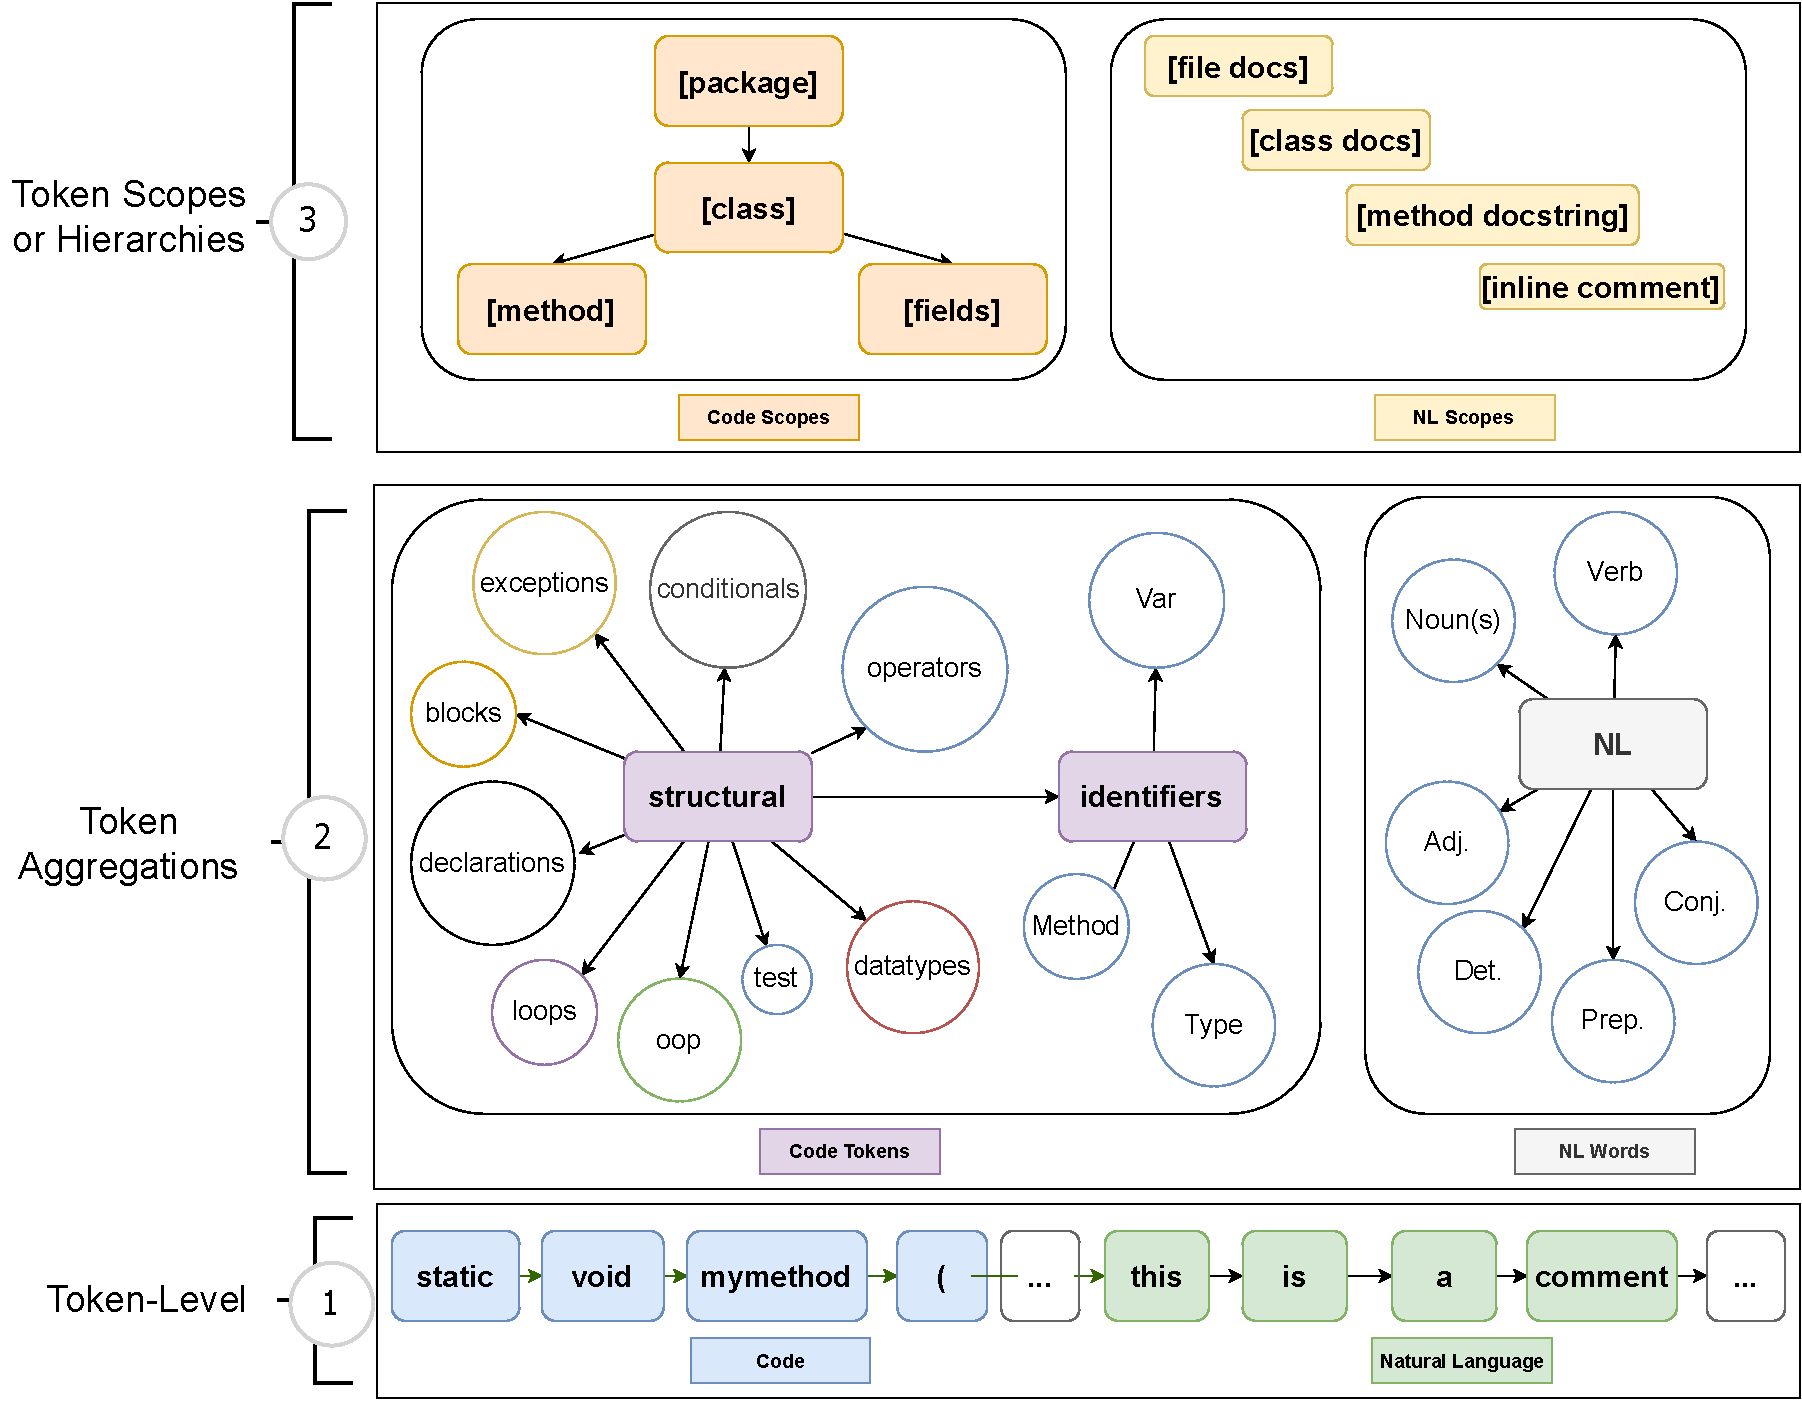
\includegraphics[width=0.9\textwidth]{graphics/chap_08-interpret-rational/fig_1_humanConcepts.pdf}
\label{fig:human}
\end{figure}


\textbf{Complexity Analysis.} In particular, Vafa et al. offer a complexity analysis for the \textit{greedy rationalization} algorithm. The analysis can be segmented in three parts: I) searching the min set of rationales in $m$ steps is $O(m)$; II) searching the max probability of $w'_t$ across $t$ is $O(t)$; and III) computing $F_{\theta}(w_t|w_{<t})$ is quadratic $O(t^2)$, in particular, for transformers. Note that in each step of the greedy rationalization, the term $F_{\theta}(w'_t|w_{r_w})$ must be evaluated, which means a complexity of $O(m^2)$ for a rationale size $m = |r|$. Therefore, if it is assumed that $m < t$, then the greedy rationalization is completed altogether in $O(m^3t)$ steps. Bear in mind that evaluating a transformer for an input $t$ would require $O(t^2)$; greedy rationalization has the same asymptotic complexity as evaluating a transformer if the rationale size $m=t^{1/3}$.

\subsection{Local post-hoc code rationales}

Most NLMs operate upon features, such as a token prediction $P(w_t|h_t)$, that do not \textit{inherently} match high-level concepts a human can easily understand. Such difficulty can be expressed mathematically as representing the state of a machine learning (ML) model as a vector space $\Vec{l}$, which corresponds to data as input features $\mathcal{S} = w_{1:T}$. Conversely, developers operate in a different vector space $\Vec{h}$, which corresponds to a set of human-interpretable concepts $\mathcal{H}$. Interpreting an $P_{\theta}$ model can be formalized as:

\begin{equation}
\phi: \Vec{l} \to \Vec{h}
\label{eq:kim}
\end{equation}

The function $\phi$ is known as \textit{function for interpretability} \citep{Kim2018InterpretabilityTCAV}. This function could adopt many forms (e.g., linear, quadratic, or polynomial) and, therefore, it may not capture all the aspects of its input domain, $\Vec{l} \in \mathcal{S}$, and it may not cover all possible human concepts in $\Vec{h} \in \mathcal{H}$. 

Post-hoc explanations occur after training a code generator $\mathcal{G}_c$. A local post-hoc explanation is the result of the interpretability function $\phi(\mathcal{S},\mathcal{H})$ for a single code sequence $\mathcal{S}$ in terms of \textbf{Human-interpretable concept} $\mathcal{H}$. \equaref{fig:human} shows three levels of human-interpretable concepts: 1) token-level, 2) token aggregations, and 3) token scopes (or hierarchies). In fact, the function \equaref{eq:kim} can be virtually \textit{code rationales} with the form $\phi_0(w_{1:T}, \mathcal{H}^{(0)}) = r(w_{1:T})$ if we consider a rationale a \textit{human-interpretable concept} $\mathcal{H}^{(0)}$. Then, $\phi_0$ would be pure analyses of rationales at token-level. 

However, we could define an extra layer of interpretability beyond reporting tokens within a rationale as depicted in \equaref{fig:human}. Such tokens can be organized or semantically grouped by their function. \equaref{fig:human}-2 presents two-fold aggregation functions depending upon the nature of tokens: code or natural language. Particularly, we proposed a \textit{structural code taxonomy for java} as a first attempt to locally aggregate code rationales $r(\mathcal{S})$ by structural categories (see \equaref{fig:taxonomy}). These categories $\mathcal{H}^{(1)}$ are high-level properties of code that can be mapped from token-level rationales. Using this taxonomy, we are able to interpret NLM predictions in a developer-centric way. In programming languages (PL), different types of tokens retain different semantic meanings. For instance $=$ and $<$ are common \textit{operators}. As such, we can group tokens into semantically meaningful categories that we call \textit{structural concepts} (see \equaref{fig:human}-2). These features will allow us to assign semantic meaning to results when analyzing rationales $r$ by defining 

\begin{align}
\begin{split}
\phi_1(\mathcal{S}, [\mathcal{H}^{(0)},  \mathcal{H}^{(1)}])  & = \lambda_{\mathcal{H}^{(1)} } ( \phi_0(\mathcal{S}, \mathcal{H}^{(0)} ) \\
                                                            & = \lambda_{\mathcal{H}^{(1)} } ( r(\mathcal{S}) )
\end{split}
\label{eq:structuralagg}
\end{align}

The mapping function $\lambda_{\mathcal{H}^{(1)}}$ receives a set of rationales of a concrete sequence $\mathcal{S}$ to generate a local explanation in terms of the structural code taxonomy. This explanation is obtained by aggregating rationales by the categories defined in the taxonomy throughout descriptive statistical function (e.g., mean, median, max, etc). Note that new taxonomies for different PLs can be derived/used. The mapping function $\lambda_{\mathcal{H}^{(1)}}$ is, indeed, a parser. This parser could translate or identify categories for a given token (e.g., operators, blocks, or loops) or word (e.g., verb, noun, or adjective). 

We can even go a little bit further and define code concepts by extracting and grouping topics from identifiers (natural language) (see \equaref{fig:human}-2). We refer to these taxonomy as \textbf{Identifier Concepts} $\mathcal{H}^{(2)}$. Here, the mapping function $\lambda_{\mathcal{H}^{(2)}}$ can be defined as an unsupervised approach to generate clusters from semantic embedded in variable names and comments. 



\textbf{Code Context Scopes} $\mathcal{H}^{(3)}$ are other type of suggested taxonomy (see \equaref{fig:human}-3). Oftentimes, it is difficult to predict whether a given NLM will be used in a similar setting to its corresponding sanitized training or testing set. For instance, if a model trained on a well-commented dataset is applied to predict segments of poorly commented code, this could potentially impact performance. As such, we define \textit{Code Context Scopes} to better understand model performance across different hierarchies or levels of context windows.  We formulate these interpretable settings as testbeds (\ie datasets) organized in context scopes. For instance, a testbed oriented to "method scope", may consist of testbeds with such level. Therefore, these datasets describe the Long Range Code Dependency property, which we introduced in the background section. Currently, \codeSeqRational supports both code and natural language scopes. For code scopes $\lambda_{\mathcal{H}^{(3)}}$, four elements are identified: (i) package, (ii) class, (iii) method, and (iv) fields (see \equaref{fig:human}-3). We can also extent the scopes to include signatures or higher level components. We support also custom mapping functions could aggregate tokens at different scopes, highlighting specific parts of the input that are particularly interesting for the downstream task at hand. For example, tokens belonging to a specific method could be aggregated in a specific category (different to other methods), if that method within has a particular role in the taks (\eg a \textit{focal} method for test generation task, a \textit{buggy} method in program repair task).

Following the same logic, other type of categories can be defined in terms of scopes without necessarily implying code hierarchies. We also introduce \textbf{Natural Language-Based Scopes} $\mathcal{H}^{(4)}$ that aggregate code rationales by file docs, class docs, method docstring, and inline comments (see \equaref{fig:human}-3). We may use a distinct mapping function $\lambda_{\mathcal{H}^{(4)}}$ based on code parser as well. 

\subsection{Global post-hoc code rationales}

Global explanations $\Phi(g,\mathcal{S}^n)$ are relevant to understand the overall behavior of a neural language model $\mathcal{G}_c$. We must define an aggregation function $g(\phi,\mathcal{S}^n)$ and a sample $n$ of sequences $\mathcal{S}^n$. Aggregation functions might vary depending on the desired statistical treatment. Even thought, global methods should always describe how input features impact model predictions on average. We suggest, in fact, employing expected values:

\begin{equation}
\Phi(g,\mathcal{S}^n,\mathcal{H}) =  g(\phi_{\mathcal{H}},\mathcal{S}^n) = \frac{1}{n} \sum_{j=1}^{n} \phi_{\mathcal{H}}(\mathcal{S}^j,\mathcal{H})
\label{eq:aggregation}
\end{equation}

Note that global explanations can be tuned for a specific \textit{human-interpretable concept} $\mathcal{H}$. We can observe how, for example, \textit{structural code} categories affect the overall prediction behavior for a given model $\mathcal{G}$. 

%------------------------------------------------

\section{Applications}
\label{sec:applications-rationales}

Although \textit{interpretability} is about \textit{why} a prediction or model decision was made, our approach supports two main applications for interpretability of NLM for code-related tasks: \textit{debugging} and \textit{optimization}. These applications can be used by researchers and practitioners designing NLM-based solutions.

\subsection{Debugging}
Debugging concerns the investigation process aiming at understanding and resolving a specific problem (or bug). In this context, debugging an NLM trained on code generation task is challenging. Differently from traditional solutions based on declarative code and rules which could be investigated and modified in order to resolve a bug, an NLM-based approach has million of parameters that contribute to the generation of an output. Our approach, provides interpretability insights to link errors to specific parts of the input to the model.

%Detecting bias

\textbf{Local Scenario,} An NLM for code completion generates a personal identifiable information within a code statement. The ML engineer of the model uses \codeSeqRational to link the generated token (personal information) to the input tokens that contributed the most to this generation. The ML engineer inspects these tokens and defines rules to abstract such tokens in the training set, so that the newly trained model will avoid similar generations in the future. 


\textbf{Global Scenario.} A code generation model makes two categories of mistakes, classified as $A$ and $B$. The ML engineer of the model collects different samples for the categories  $A$ and $B$, and uses \codeSeqRational to extract rationales, aggregate them over the two sets, and extract interpretability insights from them at code context scope level. The ML engineer discovers that the errors are originated from two scopes (\eg package and class). This information is used to change the input of the model.


\subsection{Optimization}
NLM take as input a limited-size sequence of tokens, often capped at 1024 tokens, from which the model generates an output. Given the limited nature of the input size, it is fundamental that the input space is used effectively, providing the model with the important information (tokens) while minimizing noise. Recent papers have shown the importance of providing contextual information to NLM for code generation \cite{clement2021long}, but the limited-size input of the models requires engineers to carefully decide what information to incorporate in the input. Our approach can guide ML engineers on deciding which parts of the input constitute important information to include for a specific code task.

\textbf{Global Scenario.} Two NLMs have been trained for two code-related tasks $A$ and $B$. These models both take as input a source code file. However, since some source code files are quite large, the input is often truncated. The ML engineer wants to understand what parts of the input are more important for task $A$ and $B$, so that it can optimize the input for each task. Our approach is used to generate rationales and grouped them at different code scopes. The results indicate that method docstrings are particularly important for task $A$, while class information are more influential for task $B$. This information is used by the ML engineer to optimize the input for each task. 

\subsection{Insights}
Our approach can be used to validate hypotheses on feature/token importance for specific code tasks and guide model improvements. Researchers and practitioners can use \codeSeqRational to extract interpretability values, aggregate them at different levels, and test hypotheses on the influence of class of tokens on the generated output. 

%----------------------------------------------------------------------------------------
%	CHAPTER 9: CONCLUSIONS
%----------------------------------------------------------------------------------------


\chapter{Conclusion}
\label{ch:conclusion}

We presented \codegen, an interpretability method for understanding \nlms for code. \codegen combines rigorous statistical instruments and causal inference theory to give rise to contextualized SE explanations of \nlms. Additionally, we also carried out a case study evaluation using \codegen on popular \nlms, namely, RNNs, GRUs, and Transformers, to interpret global (\ie cross-entropy) and local (\ie next token predictions) performance. \codegen exposes erroneous code concepts (\eg conditionals, or loops) by examining Average Treatment Effects and refutation methods.

\david{present new information about the mathematical structures for causality}


%----------------------------------------------------------------------------------------
%	CHAPTER 10: FUTURE
%----------------------------------------------------------------------------------------

\chapter{Future Perspective}
\label{ch:future}

\david{link this research with complex systems analysis}

%----------------------------------------------------------------------------------------

%\chapter{The Design of Tufte's Books}
\label{ch:tufte-design}

\newthought{The pages} of a book are usually divided into three major sections: the front matter (also called preliminary matter or prelim), the main matter (the core text of the book), and the back matter (or end matter).

\newthought{The front matter} of a book refers to all of the material that comes before the main text. The following table shows a list of material that appears in the front matter of \VDQI, \EI, \VE, and \BE along with its page number. Page numbers that appear in parentheses refer to folios that do not have a printed page number (but they are still counted in the page number sequence).

\bigskip
\begin{minipage}{\textwidth}
\begin{center}
\begin{tabular}{lcccc}
\toprule
& \multicolumn{4}{c}{Books} \\
\cmidrule(l){2-5} 
Page content & \vdqi & \ei & \ve & \be \\
\midrule
Blank half title page & \hangp{1} & \hangp{1} & \hangp{1} & \hangp{1} \\
Frontispiece\footnotemark{}
& \hangp{2} & \hangp{2} & \hangp{2} & \hangp{2} \\
Full title page & \hangp{3} & \hangp{3} & \hangp{3} & \hangp{3} \\
Copyright page & \hangp{4} & \hangp{4} & \hangp{4} & \hangp{4} \\
Contents & \hangp{5} & \hangp{5} & \hangp{5} & \hangp{5} \\
Dedication & \hangp{6} & \hangp{7} & \hangp{7} & 7 \\
Epigraph & -- & -- & \hangp{8} & -- \\
Introduction & \hangp{7} & \hangp{9} & \hangp{9} & 9 \\
\bottomrule
\end{tabular}
\end{center}
\end{minipage}
\vspace{-7\baselineskip}\footnotetext{The contents of this page vary from book to book. In \vdqi this page is blank; in \ei and \ve this page holds a frontispiece; and in \be this page contains three epigraphs.}
\vspace{7\baselineskip}

\bigskip
The design of the front matter in Tufte's books varies slightly from the traditional design of front matter. First, the pages in front matter are traditionally numbered with lowercase roman numerals (\eg, i, ii, iii, iv,~\ldots). Second, the front matter page numbering sequence is usually separate from the main matter page numbering. That is, the page numbers restart at 1 when the main matter begins. In contrast, Tufte has enumerated his pages with arabic numerals that share the same page counting sequence as the main matter.

There are also some variations in design across Tufte's four books. The page opposite the full title page (labeled ``frontispiece'' in the above table) has different content in each of the books. In \VDQI, this page is blank; in \EI and \VE, this page holds a frontispiece; and in \BE, this page contains three epigraphs.

The dedication appears on page~6 in \vdqi (opposite the introduction), and is placed on its own spread in the other books. In \ve, an epigraph shares the spread with the opening page of the introduction.

None of the page numbers (folios) of the front matter are expressed except in \be, where the folios start to appear on the dedication page.

\newthought{The full title page} of each of the books varies slightly in design. In all the books, the author's name appears at the top of the page, the title it set just above the center line, and the publisher is printed along the bottom margin. Some of the differences are outlined in the following table.

\bigskip
\begin{center}
\footnotesize
\begin{tabular}{lllll}
\toprule
Feature & \vdqi & \ei & \ve & \be \\
\midrule
Author & & & & \\
\quad Typeface & serif & serif & serif & sans serif \\
\quad Style & italics & italics & italics & upright, caps \\
\quad Size & 24 pt & 20 pt & 20 pt & 20 pt \\
\addlinespace
Title & & & & \\
\quad Typeface & serif & serif & serif & sans serif \\
\quad Style & upright & italics & upright & upright, caps \\
\quad Size & 36 pt & 48 pt & 48 pt & 36 pt \\
\addlinespace
Subtitle & & & & \\
\quad Typeface & \na & \na & serif & \na \\
\quad Style & \na & \na & upright & \na \\
\quad Size & \na & \na & 20 pt & \na \\
\addlinespace
Edition & & & & \\
\quad Typeface & sans serif & \na & \na & \na \\
\quad Style & upright, caps & \na & \na & \na \\
\quad Size & 14 pt & \na & \na & \na \\
\addlinespace
Publisher & & & & \\
\quad Typeface & serif & serif & serif & sans serif \\
\quad Style & italics & italics & italics & upright, caps \\
\quad Size & 14 pt & 14 pt & 14 pt & 14 pt \\
\bottomrule
\end{tabular}
\end{center}

\begin{figure*}[p]
\fbox{
\includegraphics[width=0.45\linewidth]{graphics/vdqi-title.pdf}}
\hfill
\fbox{
\includegraphics[width=0.45\linewidth]{graphics/ei-title.pdf}}
\\\vspace{\baselineskip}
\fbox{
\includegraphics[width=0.45\linewidth]{graphics/ve-title.pdf}}
\hfill
\fbox{
\includegraphics[width=0.45\linewidth]{graphics/be-title.pdf}}
\end{figure*}

\newthought{The tables of contents} in Tufte's books give us our first glimpse of the structure of the main matter. \VDQI is split into two parts, each containing some number of chapters. His other three books only contain chapters---they're not broken into parts.

\begin{figure*}[p]\index{table of contents}
\fbox{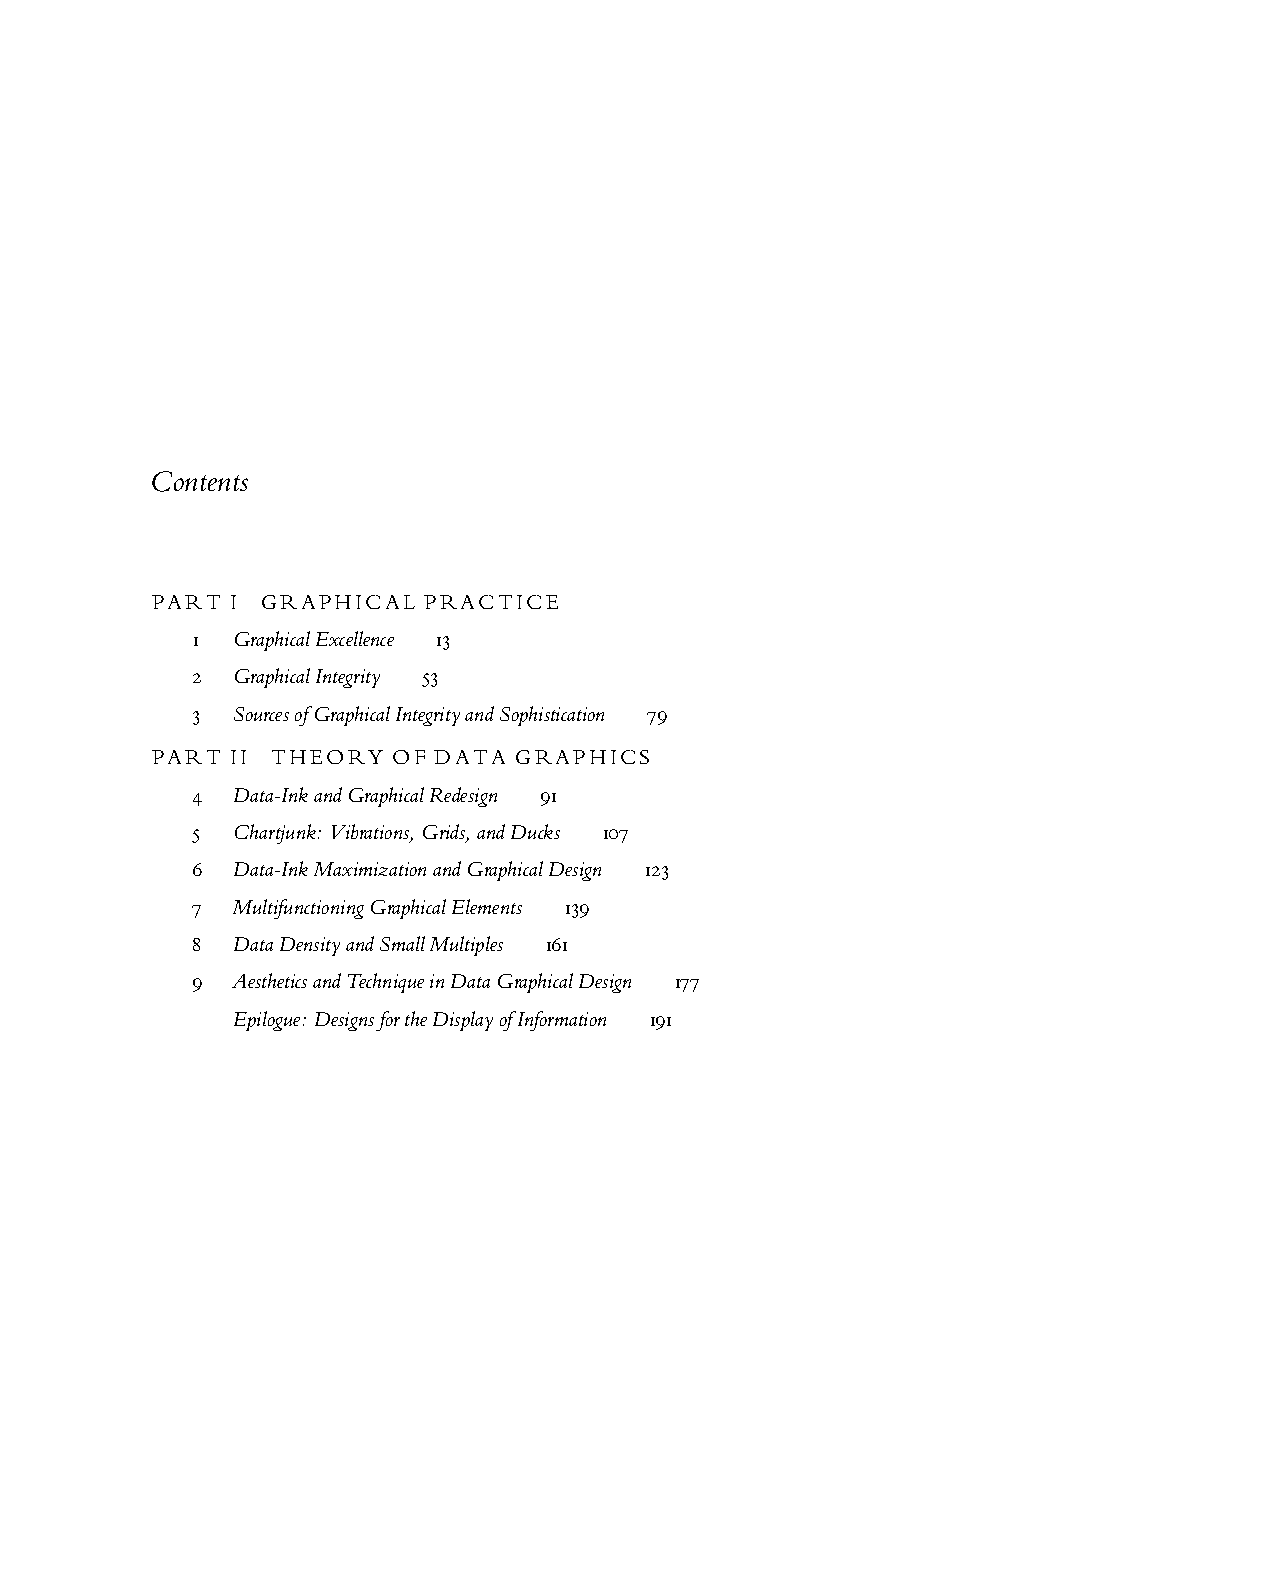
\includegraphics[width=0.45\linewidth]{graphics/vdqi-contents.pdf}}
\hfill
\fbox{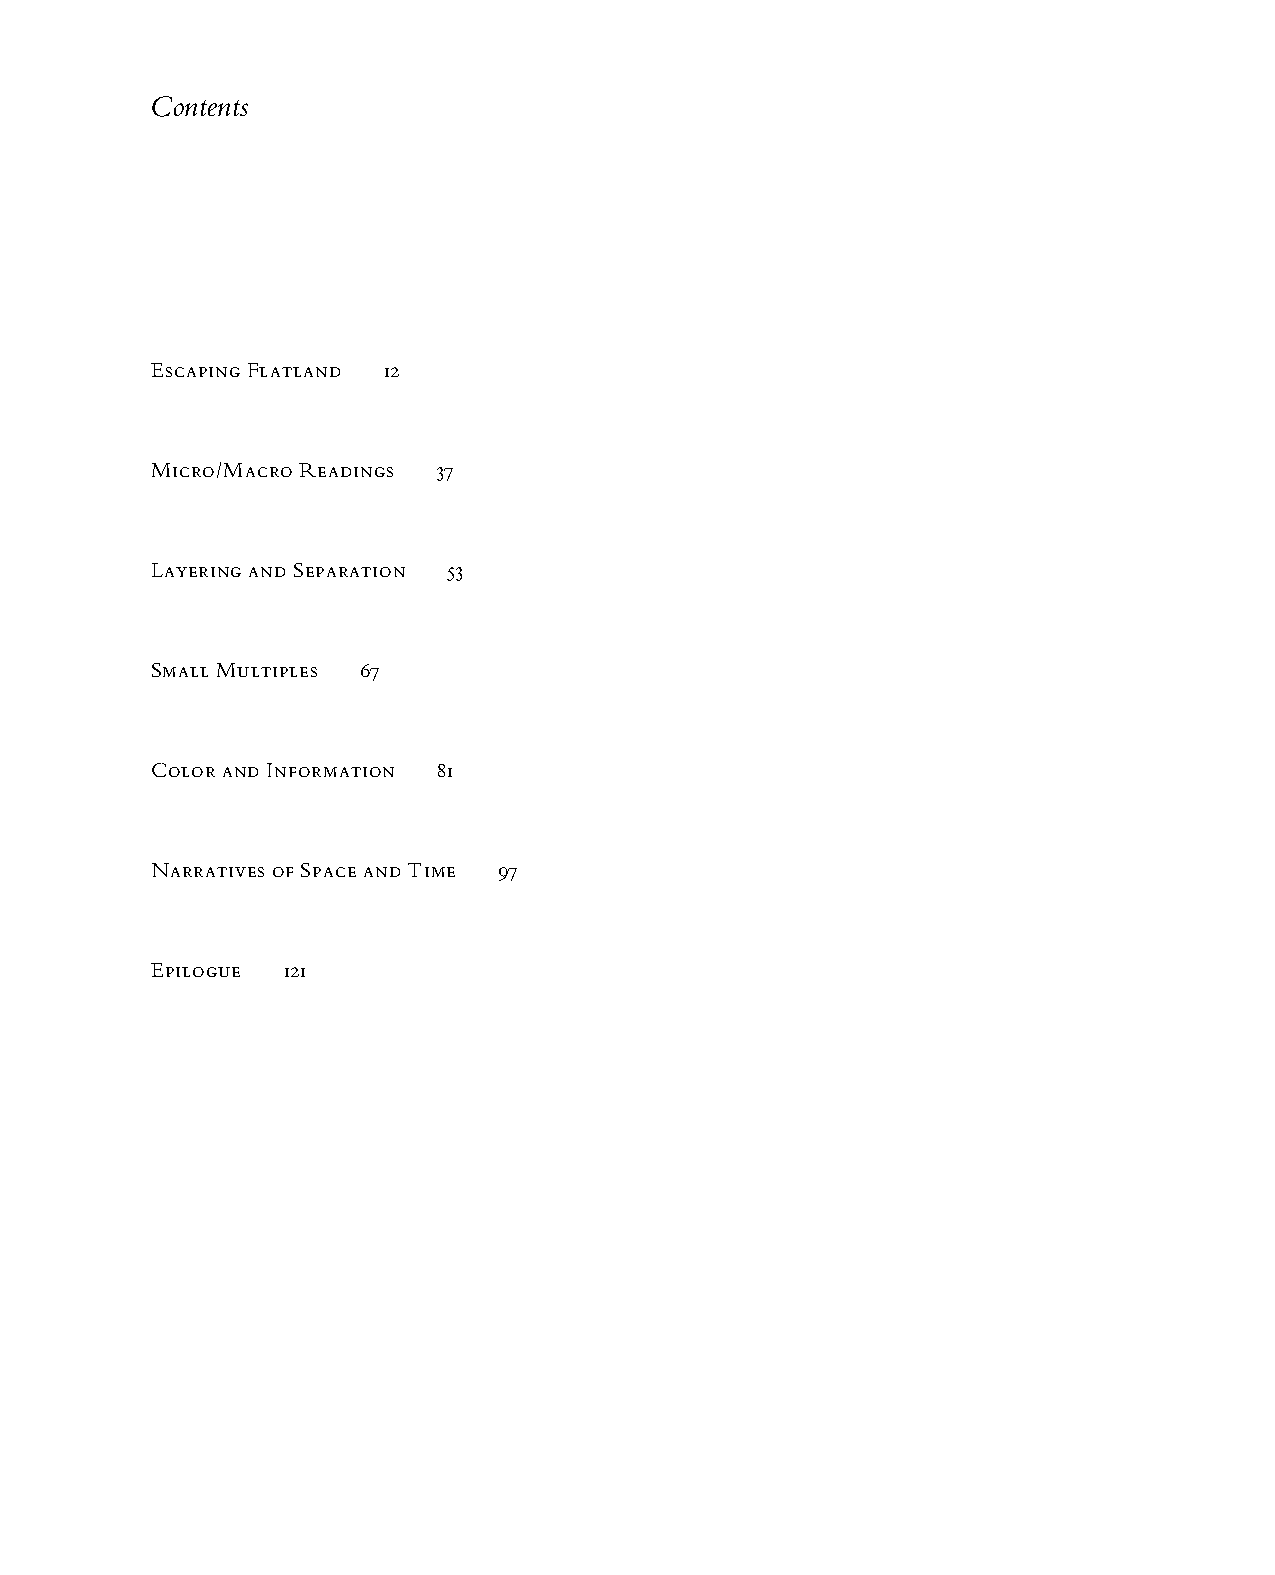
\includegraphics[width=0.45\linewidth]{graphics/ei-contents.pdf}}
\\\vspace{\baselineskip}
\fbox{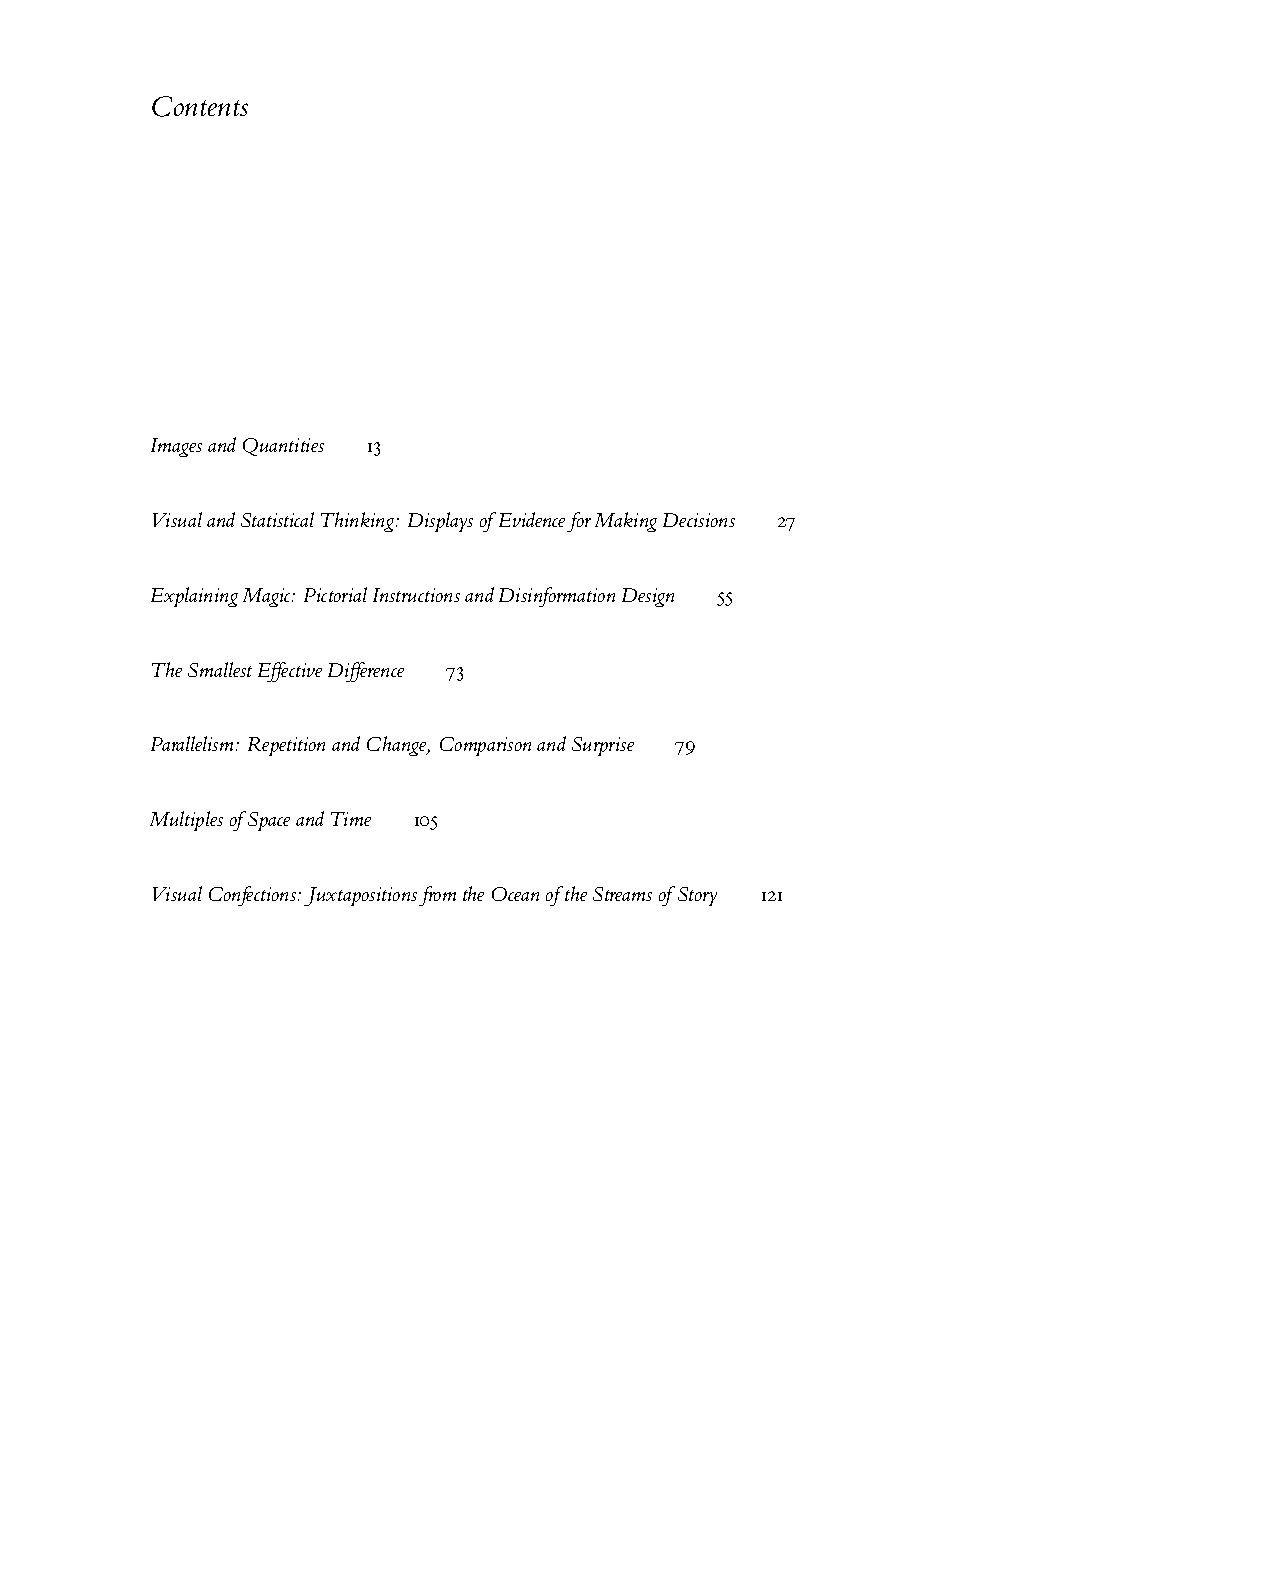
\includegraphics[width=0.45\linewidth]{graphics/ve-contents.pdf}}
\hfill
\fbox{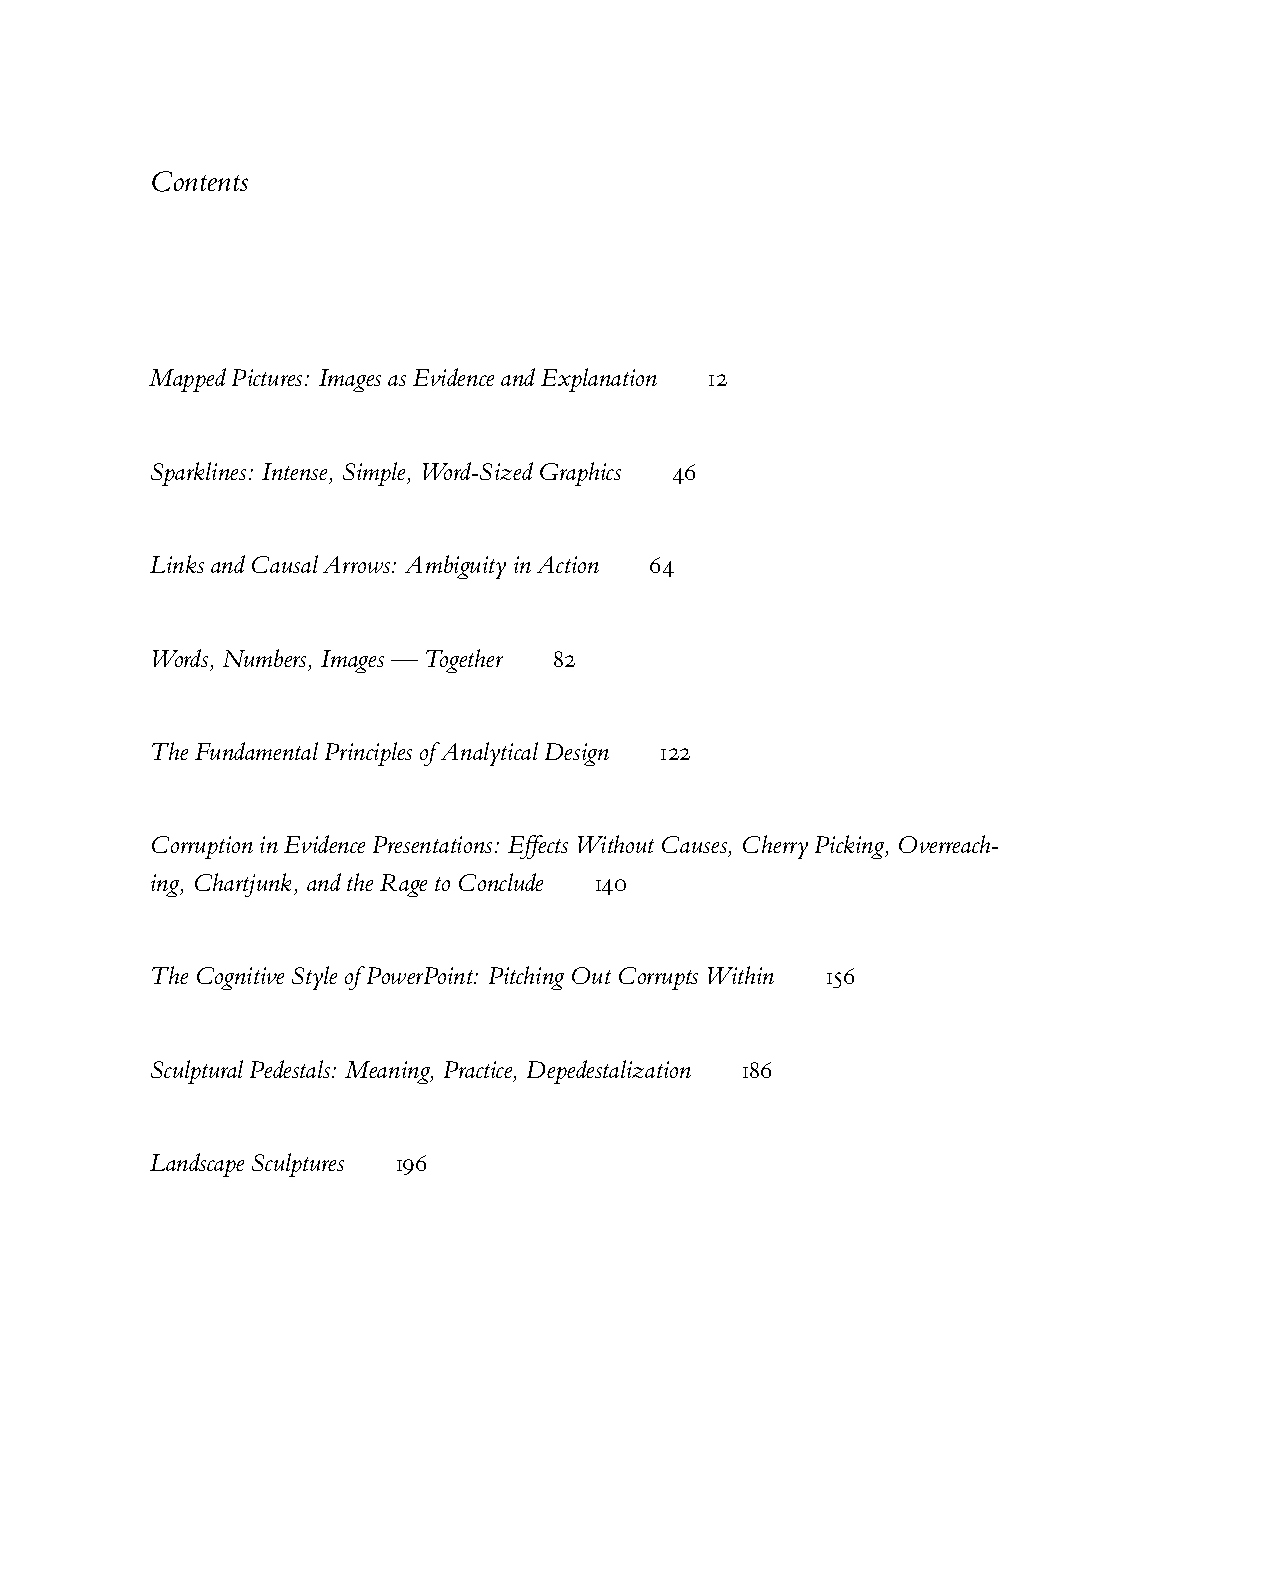
\includegraphics[width=0.45\linewidth]{graphics/be-contents.pdf}}
\end{figure*}

%------------------------------------------------

\section{Typefaces}\label{sec:typefaces1}\index{typefaces}
\index{fonts|see{typefaces}}

Tufte's books primarily use two typefaces: Bembo and Gill Sans. Bembo is used for the headings and body text, while Gill Sans is used for the title page and opening epigraphs in \BE.

Since neither Bembo nor Gill Sans are available in default \LaTeX{} installations, the \TL document classes default to using Palatino and Helvetica, respectively. In addition, the Bera Mono typeface is used for \texttt{monospaced} type.

The following font sizes are defined by the \TL classes:

\begin{table}[h]\index{typefaces!sizes}
\footnotesize%
\begin{center}
\begin{tabular}{lccl}
\toprule
\LaTeX{} size & Font size & Leading & Used for \\
\midrule
\verb+\tiny+ & 5 & 6 & sidenote numbers \\
\verb+\scriptsize+ & 7 & 8 & \na \\
\verb+\footnotesize+ & 8 & 10 & sidenotes, captions \\
\verb+\small+ & 9 & 12 & quote, quotation, and verse environments \\
\verb+\normalsize+ & 10 & 14 & body text \\
\verb+\large+ & 11 & 15 & \textsc{b}-heads \\
\verb+\Large+ & 12 & 16 & \textsc{a}-heads, \textsc{toc} entries, author, date \\
\verb+\LARGE+ & 14 & 18 & handout title \\
\verb+\huge+ & 20 & 30 & chapter heads \\
\verb+\Huge+ & 24 & 36 & part titles \\
\bottomrule
\end{tabular}
\end{center}
\caption{A list of \LaTeX{} font sizes as defined by the \TL document classes.}
\label{tab:font-sizes}
\end{table}

%------------------------------------------------

\section{Headings}\label{sec:headings1}\index{headings}

Tufte's books include the following heading levels: parts, chapters,\sidenote{Parts and chapters are defined for the \texttt{tufte-book} class only.} sections, subsections, and paragraphs. Not defined by default are: sub-subsections and subparagraphs.

\begin{table}[h]
\begin{center}
\footnotesize
\begin{tabular}{lcr}
\toprule
Heading & Style & Size \\
\midrule
Part & roman & \measure{24}{36}{40} \\
Chapter & italic & \measure{20}{30}{40} \\
Section & italic & \measure{12}{16}{26} \\
Subsection & italic & \measure{11}{15}{26} \\
Paragraph & italic & 10/14 \\
\bottomrule
\end{tabular}
\end{center}
\caption{Heading styles used in \BE.}
\label{tab:heading-styles}
\end{table}

\paragraph{Paragraph} Paragraph headings (as shown here) are introduced by italicized text and separated from the main paragraph by a bit of space.

%------------------------------------------------

\section{Environments}

The following characteristics define the various environments:

\begin{table}[h]
\begin{center}
\footnotesize
\begin{tabular}{lcl}
\toprule
Environment & Font size & Notes \\
\midrule
Body text & \measure{10}{14}{26} & \\
Block quote & \measure{9}{12}{24} & Block indent (left and right) by \unit[1]{pc} \\
Sidenotes & \measure{8}{10}{12} & Sidenote number is set inline, followed by word space \\
Captions & \measure{8}{10}{12} & \\
\bottomrule
\end{tabular}
\end{center}
\caption{Environment styles used in \BE.}
\label{tab:environment-styles}
\end{table}

%----------------------------------------------------------------------------------------
%	CHAPTER 2
%----------------------------------------------------------------------------------------

\chapter[On the Use of the tufte-book Document Class]{On the Use of the \texttt{tufte-book} Document Class}
\label{ch:tufte-book}

The \TL document classes define a style similar to the style Edward Tufte uses in his books and handouts. Tufte's style is known for its extensive use of sidenotes, tight integration of graphics with text, and well-set typography. This document aims to be at once a demonstration of the features of the \TL document classes and a style guide to their use.

%------------------------------------------------

\section{Page Layout}\label{sec:page-layout}
\subsection{Headings}\label{sec:headings}\index{headings}
This style provides \textsc{a}- and \textsc{b}-heads (that is, \Verb|\section| and \Verb|\subsection|), demonstrated above.

If you need more than two levels of section headings, you'll have to define them yourself at the moment; there are no pre-defined styles for anything below a \Verb|\subsection|. As Bringhurst points out in \textit{The Elements of Typographic Style},\cite{Bringhurst2005} you should ``use as many levels of headings as you need: no more, and no fewer.''

The \TL classes will emit an error if you try to use \linebreak\Verb|\subsubsection| and smaller headings.

\newthought{In his later books},\cite{Tufte2006} Tufte starts each section with a bit of vertical space, a non-indented paragraph, and sets the first few words of the sentence in \textsc{small caps}. To accomplish this using this style, use the \doccmddef{newthought} command:
\begin{docspec}
\doccmd{newthought}\{In his later books\}, Tufte starts\ldots
\end{docspec}

%------------------------------------------------

\section{Sidenotes}\label{sec:sidenotes}
One of the most prominent and distinctive features of this style is the extensive use of sidenotes. There is a wide margin to provide ample room for sidenotes and small figures. Any \doccmd{footnote}s will automatically be converted to sidenotes.\footnote{This is a sidenote that was entered using the \texttt{\textbackslash footnote} command.} If you'd like to place ancillary information in the margin without the sidenote mark (the superscript number), you can use the \doccmd{marginnote} command.\marginnote{This is a margin note. Notice that there isn't a number preceding the note, and there is no number in the main text where this note was written.}

The specification of the \doccmddef{sidenote} command is:
\begin{docspec}
\doccmd{sidenote}[\docopt{number}][\docopt{offset}]\{\docarg{Sidenote text.}\}
\end{docspec}

Both the \docopt{number} and \docopt{offset} arguments are optional. If you provide a \docopt{number} argument, then that number will be used as the sidenote number. It will change of the number of the current sidenote only and will not affect the numbering sequence of subsequent sidenotes.

Sometimes a sidenote may run over the top of other text or graphics in the margin space. If this happens, you can adjust the vertical position of the sidenote by providing a dimension in the \docopt{offset} argument. Some examples of valid dimensions are:
\begin{docspec}
\ttfamily 1.0in \qquad 2.54cm \qquad 254mm \qquad 6\Verb|\baselineskip|
\end{docspec}
If the dimension is positive it will push the sidenote down the page; if the dimension is negative, it will move the sidenote up the page.

While both the \docopt{number} and \docopt{offset} arguments are optional, they must be provided in order. To adjust the vertical position of the sidenote while leaving the sidenote number alone, use the following syntax:
\begin{docspec}
\doccmd{sidenote}[][\docopt{offset}]\{\docarg{Sidenote text.}\}
\end{docspec}
The empty brackets tell the \Verb|\sidenote| command to use the default sidenote number.

If you \emph{only} want to change the sidenote number, however, you may completely omit the \docopt{offset} argument:
\begin{docspec}
\doccmd{sidenote}[\docopt{number}]\{\docarg{Sidenote text.}\}
\end{docspec}

The \doccmddef{marginnote} command has a similar \docarg{offset} argument:
\begin{docspec}
\doccmd{marginnote}[\docopt{offset}]\{\docarg{Margin note text.}\}
\end{docspec}

%------------------------------------------------

\section{References}
References are placed alongside their citations as sidenotes, as well. This can be accomplished using the normal \doccmddef{cite} command.\sidenote{The first paragraph of this document includes a citation.}

The complete list of references may also be printed automatically by using the \doccmddef{bibliography} command. (See the end of this document for an example.) If you do not want to print a bibliography at the end of your document, use the \doccmddef{nobibliography} command in its place. 

To enter multiple citations at one location,\cite[-3\baselineskip]{Tufte2006,Tufte1990} you can provide a list of keys separated by commas and the same optional vertical offset argument: \Verb|\cite{Tufte2006,Tufte1990}|. 
\begin{docspec}
\doccmd{cite}[\docopt{offset}]\{\docarg{bibkey1,bibkey2,\ldots}\}
\end{docspec}

%------------------------------------------------

\section{Figures and Tables}\label{sec:figures-and-tables}
Images and graphics play an integral role in Tufte's work. In addition to the standard \docenvdef{figure} and \docenvdef{tabular} environments, this style provides special figure and table environments for full-width floats.

Full page--width figures and tables may be placed in \docenvdef{figure*} or \docenvdef{table*} environments. To place figures or tables in the margin, use the \docenvdef{marginfigure} or \docenvdef{margintable} environments as follows (see figure~\ref{fig:marginfig}):

\begin{marginfigure}
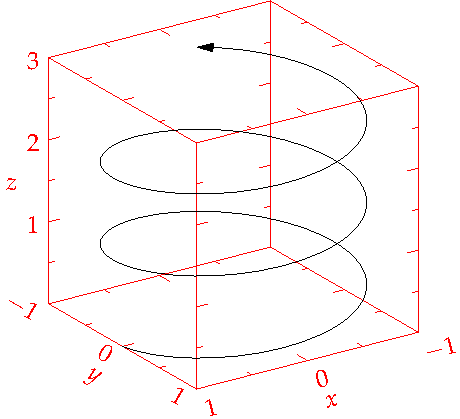
\includegraphics[width=\linewidth]{helix}
\caption{This is a margin figure. The helix is defined by $x = \cos(2\pi z)$, $y = \sin(2\pi z)$, and $z = [0, 2.7]$. The figure was drawn using Asymptote (\url{http://asymptote.sf.net/}).}
\label{fig:marginfig}
\end{marginfigure}

\begin{docspec}
\textbackslash begin\{marginfigure\}\\
\qquad\textbackslash includegraphics\{helix\}\\
\qquad\textbackslash caption\{This is a margin figure.\}\\
\qquad\textbackslash label\{fig:marginfig\}\\
\textbackslash end\{marginfigure\}\\
\end{docspec}

The \docenv{marginfigure} and \docenv{margintable} environments accept an optional parameter \docopt{offset} that adjusts the vertical position of the figure or table. See the ``\nameref{sec:sidenotes}'' section above for examples. The specifications are:
\begin{docspec}
\textbackslash{begin\{marginfigure\}[\docopt{offset}]}\\
\qquad\ldots\\
\textbackslash{end\{marginfigure\}}\\
\mbox{}\\
\textbackslash{begin\{margintable\}[\docopt{offset}]}\\
\qquad\ldots\\
\textbackslash{end\{margintable\}}\\
\end{docspec}

Figure~\ref{fig:fullfig} is an example of the \docenv{figure*} environment and figure~\ref{fig:textfig} is an example of the normal \docenv{figure} environment.

\begin{figure*}[h]
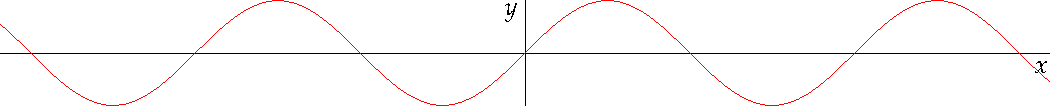
\includegraphics[width=\linewidth]{sine.pdf}
\caption{This graph shows $y = \sin x$ from about $x = [-10, 10]$.
\emph{Notice that this figure takes up the full page width.}}
\label{fig:fullfig}
\end{figure*}

\begin{figure}
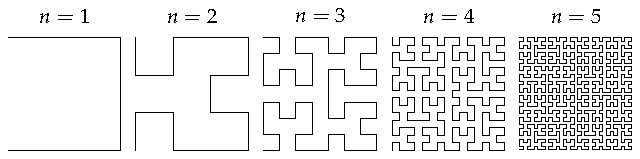
\includegraphics{hilbertcurves.pdf}
\caption[Hilbert curves of various degrees $n$.][6pt]{Hilbert curves of various degrees $n$. \emph{Notice that this figure only takes up the main textblock width.}}
\label{fig:textfig}
\end{figure}

As with sidenotes and marginnotes, a caption may sometimes require vertical adjustment. The \doccmddef{caption} command now takes a second optional argument that enables you to do this by providing a dimension \docopt{offset}. You may specify the caption in any one of the following forms:
\begin{docspec}
\doccmd{caption}\{\docarg{long caption}\}\\
\doccmd{caption}[\docarg{short caption}]\{\docarg{long caption}\}\\
\doccmd{caption}[][\docopt{offset}]\{\docarg{long caption}\}\\
\doccmd{caption}[\docarg{short caption}][\docopt{offset}]%
\{\docarg{long caption}\}
\end{docspec}
A positive \docopt{offset} will push the caption down the page. The short caption, if provided, is what appears in the list of figures/tables, otherwise the ``long'' caption appears there. Note that although the arguments \docopt{short caption} and \docopt{offset} are both optional, they must be provided in order. Thus, to specify an \docopt{offset} without specifying a \docopt{short caption}, you must include the first set of empty brackets \Verb|[]|, which tell \doccmd{caption} to use the default ``long'' caption. As an example, the caption to figure~\ref{fig:textfig} above was given in the form
\begin{docspec}
\doccmd{caption}[Hilbert curves...][6pt]\{Hilbert curves...\}
\end{docspec}

Table~\ref{tab:normaltab} shows table created with the \docpkg{booktabs} package. Notice the lack of vertical rules---they serve only to clutter the table's data.

\begin{table}[ht]
\centering
\fontfamily{ppl}\selectfont
\begin{tabular}{ll}
\toprule
Margin & Length \\
\midrule
Paper width & \unit[8\nicefrac{1}{2}]{inches} \\
Paper height & \unit[11]{inches} \\
Textblock width & \unit[6\nicefrac{1}{2}]{inches} \\
Textblock/sidenote gutter & \unit[\nicefrac{3}{8}]{inches} \\
Sidenote width & \unit[2]{inches} \\
\bottomrule
\end{tabular}
\caption{Here are the dimensions of the various margins used in the Tufte-handout class.}
\label{tab:normaltab}
\end{table}

\newthought{Occasionally} \LaTeX{} will generate an error message:\label{err:too-many-floats}
\begin{docspec}
Error: Too many unprocessed floats
\end{docspec}
\LaTeX{} tries to place floats in the best position on the page. Until it's finished composing the page, however, it won't know where those positions are. If you have a lot of floats on a page (including sidenotes, margin notes, figures, tables, etc.), \LaTeX{} may run out of ``slots'' to keep track of them and will generate the above error.

\LaTeX{} initially allocates 18 slots for storing floats. To work around this limitation, the \TL document classes provide a \doccmddef{morefloats} command that will reserve more slots.

The first time \doccmd{morefloats} is called, it allocates an additional 34 slots. The second time \doccmd{morefloats} is called, it allocates another 26 slots.

The \doccmd{morefloats} command may only be used two times. Calling it a third time will generate an error message. (This is because we can't safely allocate many more floats or \LaTeX{} will run out of memory.)

If, after using the \doccmd{morefloats} command twice, you continue to get the \texttt{Too many unprocessed floats} error, there are a couple things you can do.

The \doccmddef{FloatBarrier} command will immediately process all the floats before typesetting more material. Since \doccmd{FloatBarrier} will start a new paragraph, you should place this command at the beginning or end of a paragraph.

The \doccmddef{clearpage} command will also process the floats before continuing, but instead of starting a new paragraph, it will start a new page.

You can also try moving your floats around a bit: move a figure or table to the next page or reduce the number of sidenotes. (Each sidenote actually uses \emph{two} slots.)

After the floats have placed, \LaTeX{} will mark those slots as unused so they are available for the next page to be composed.

%------------------------------------------------

\section{Captions}
You may notice that the captions are sometimes misaligned. Due to the way \LaTeX's float mechanism works, we can't know for sure where it decided to put a float. Therefore, the \TL document classes provide commands to override the caption position.

\paragraph{Vertical alignment} To override the vertical alignment, use the \doccmd{setfloatalignment} command inside the float environment. For example:

\begin{fullwidth}
\begin{docspec}
\textbackslash begin\{figure\}[btp]\\
\qquad \textbackslash includegraphics\{sinewave\}\\
\qquad \textbackslash caption\{This is an example of a sine wave.\}\\
\qquad \textbackslash label\{fig:sinewave\}\\
\qquad \hlred{\textbackslash setfloatalignment\{b\}\% forces caption to be bottom-aligned}\\
\textbackslash end\{figure\}
\end{docspec}
\end{fullwidth}

\noindent The syntax of the \doccmddef{setfloatalignment} command is:

\begin{docspec}
\doccmd{setfloatalignment}\{\docopt{pos}\}
\end{docspec}

\noindent where \docopt{pos} can be either \texttt{b} for bottom-aligned captions, or \texttt{t} for top-aligned captions.

\paragraph{Horizontal alignment}\label{par:overriding-horizontal}
To override the horizontal alignment, use either the \doccmd{forceversofloat} or the \doccmd{forcerectofloat} command inside of the float environment. For example:

\begin{fullwidth}
\begin{docspec}
\textbackslash begin\{figure\}[btp]\\
\qquad \textbackslash includegraphics\{sinewave\}\\
\qquad \textbackslash caption\{This is an example of a sine wave.\}\\
\qquad \textbackslash label\{fig:sinewave\}\\
\qquad \hlred{\textbackslash forceversofloat\% forces caption to be set to the left of the float}\\
\textbackslash end\{figure\}
\end{docspec}
\end{fullwidth}

The \doccmddef{forceversofloat} command causes the algorithm to assume the float has been placed on a verso page---that is, a page on the left side of a two-page spread. Conversely, the \doccmddef{forcerectofloat} command causes the algorithm to assume the float has been placed on a recto page---that is, a page on the right side of a two-page spread.

%------------------------------------------------

\section{Full-width text blocks}

In addition to the new float types, there is a \docenvdef{fullwidth} environment that stretches across the main text block and the sidenotes area.

\begin{Verbatim}
\begin{fullwidth}
Lorem ipsum dolor sit amet...
\end{fullwidth}
\end{Verbatim}

\begin{fullwidth}
\small\itshape\lipsum[1]
\end{fullwidth}

%------------------------------------------------

\section{Typography}\label{sec:typography}

\subsection{Typefaces}\label{sec:typefaces}\index{typefaces}
If the Palatino, \textsf{Helvetica}, and \texttt{Bera Mono} typefaces are installed, this style will use them automatically. Otherwise, we'll fall back on the Computer Modern typefaces.

\subsection{Letterspacing}\label{sec:letterspacing}
This document class includes two new commands and some improvements on existing commands for letterspacing.

When setting strings of \allcaps{ALL CAPS} or \smallcaps{small caps}, the letter\-spacing---that is, the spacing between the letters---should be increased slightly.\cite{Bringhurst2005} The \doccmddef{allcaps} command has proper letterspacing for strings of \allcaps{FULL CAPITAL LETTERS}, and the \doccmddef{smallcaps} command has letterspacing for \smallcaps{small capital letters}. These commands will also automatically convert the case of the text to upper- or lowercase, respectively.

The \doccmddef{textsc} command has also been redefined to include letterspacing. The case of the \doccmd{textsc} argument is left as is, however. This allows one to use both uppercase and lowercase letters: \textsc{The Initial Letters Of The Words In This Sentence Are Capitalized.}

%------------------------------------------------

\section{Document Class Options}\label{sec:options}

\index{class options|(}
The \doccls{tufte-book} class is based on the \LaTeX\ \doccls{book} document class. Therefore, you can pass any of the typical book options. There are a few options that are specific to the \doccls{tufte-book} document class, however.

The \docclsoptdef{a4paper} option will set the paper size to \smallcaps{A4} instead of the default \smallcaps{US} letter size.

The \docclsoptdef{sfsidenotes} option will set the sidenotes and title block in a \textsf{sans serif} typeface instead of the default roman.

The \docclsoptdef{twoside} option will modify the running heads so that the page number is printed on the outside edge (as opposed to always printing the page number on the right-side edge in \docclsoptdef{oneside} mode). 

The \docclsoptdef{symmetric} option typesets the sidenotes on the outside edge of the page. This is how books are traditionally printed, but is contrary to Tufte's book design which sets the sidenotes on the right side of the page. This option implicitly sets the \docclsopt{twoside} option.

The \docclsoptdef{justified} option sets all the text fully justified (flush left and right). The default is to set the text ragged right. The body text of Tufte's books are set ragged right. This prevents needless hyphenation and makes it easier to read the text in the slightly narrower column.

The \docclsoptdef{bidi} option loads the \docpkg{bidi} package which is used with \tXeLaTeX\ to typeset bi-directional text. Since the \docpkg{bidi} package needs to be loaded before the sidenotes and cite commands are defined, it can't be loaded in the document preamble.

The \docclsoptdef{debug} option causes the \TL classes to output debug information to the log file which is useful in troubleshooting bugs. It will also cause the graphics to be replaced by outlines.

The \docclsoptdef{nofonts} option prevents the \TL classes from automatically loading the Palatino and Helvetica typefaces. You should use this option if you wish to load your own fonts. If you're using \tXeLaTeX, this option is implied (\ie, the Palatino and Helvetica fonts aren't loaded if you use \tXeLaTeX). 

The \docclsoptdef{nols} option inhibits the letterspacing code. The \TL\ classes try to load the appropriate letterspacing package (either pdf\TeX's \docpkg{letterspace} package or the \docpkg{soul} package). If you're using \tXeLaTeX\ with \docpkg{fontenc}, however, you should configure your own letterspacing. 

The \docclsoptdef{notitlepage} option causes \doccmd{maketitle} to generate a title block instead of a title page. The \doccls{book} class defaults to a title page and the \doccls{handout} class defaults to the title block. There is an analogous \docclsoptdef{titlepage} option that forces \doccmd{maketitle} to generate a full title page instead of the title block.

The \docclsoptdef{notoc} option suppresses \TL's custom table of contents (\textsc{toc}) design. The current \textsc{toc} design only shows unnumbered chapter titles; it doesn't show sections or subsections. The \docclsopt{notoc} option will revert to \LaTeX's \textsc{toc} design.

The \docclsoptdef{nohyper} option prevents the \docpkg{hyperref} package from being loaded. The default is to load the \docpkg{hyperref} package and use the \doccmd{title} and \doccmd{author} contents as metadata for the generated \textsc{pdf}.

\index{class options|)}

%----------------------------------------------------------------------------------------
%	CHAPTER 3
%----------------------------------------------------------------------------------------

\chapter[Customizing Tufte-LaTeX]{Customizing \TL}
\label{ch:customizing}

The \TL document classes are designed to closely emulate Tufte's book design by default. However, each document is different and you may encounter situations where the default settings are insufficient. This chapter explores many of the ways you can adjust the \TL document classes to better fit your needs.

%------------------------------------------------

\section{File Hooks}
\label{sec:filehooks}

\index{file hooks|(}
If you create many documents using the \TL classes, it's easier to store your customizations in a separate file instead of copying them into the preamble of each document. The \TL classes provide three file hooks: \docfilehook{tufte-common-local.tex}{common}, \docfilehook{tufte-book-local.tex}{book}, and \docfilehook{tufte-handout-local.tex}{handout}.\sloppy

\begin{description}
\item[\docfilehook{tufte-common-local.tex}{common}]
If this file exists, it will be loaded by all of the \TL document classes just prior to any document-class-specific code. If your customizations or code should be included in both the book and handout classes, use this file hook.
\item[\docfilehook{tufte-book-local.tex}{book}] 
If this file exists, it will be loaded after all of the common and book-specific code has been read. If your customizations apply only to the book class, use this file hook.
\item[\docfilehook{tufte-common-handout.tex}{handout}] 
If this file exists, it will be loaded after all of the common and handout-specific code has been read. If your customizations apply only to the handout class, use this file hook.
\end{description}

\index{file hooks|)}

%------------------------------------------------

\section{Numbered Section Headings}
\label{sec:numbered-sections}
\index{headings!numbered}

While Tufte dispenses with numbered headings in his books, if you require them, they can be enabled by changing the value of the \doccounter{secnumdepth} counter. From the table below, select the heading level at which numbering should stop and set the \doccounter{secnumdepth} counter to that value. For example, if you want parts and chapters numbered, but don't want numbering for sections or subsections, use the command:
\begin{docspec}
\doccmd{setcounter}\{secnumdepth\}\{0\}
\end{docspec}

The default \doccounter{secnumdepth} for the \TL document classes is $-1$.

\begin{table}
\footnotesize
\begin{center}
\begin{tabular}{lr}
\toprule
Heading level & Value \\
\midrule
Part (in \doccls{tufte-book}) & $-1$ \\
Part (in \doccls{tufte-handout}) & $0$ \\
Chapter (only in \doccls{tufte-book}) & $0$ \\
Section & $1$ \\
Subsection & $2$ \\
Subsubsection & $3$ \\
Paragraph & $4$ \\
Subparagraph & $5$ \\
\bottomrule
\end{tabular}
\end{center}
\caption{Heading levels used with the \texttt{secnumdepth} counter.}
\end{table}

%------------------------------------------------

\section{Changing the Paper Size}
\label{sec:paper-size}

The \TL classes currently only provide three paper sizes: \textsc{a4}, \textsc{b5}, and \textsc{us} letter. To specify a different paper size (and/or margins), use the \doccmd[geometry]{geometrysetup} command in the preamble of your document (or one of the file hooks). The full documentation of the \doccmd{geometrysetup} command may be found in the \docpkg{geometry} package documentation.\cite{pkg-geometry}

%------------------------------------------------

\section{Customizing Marginal Material}
\label{sec:marginal-material}

Marginal material includes sidenotes, citations, margin notes, and captions. Normally, the justification of the marginal material follows the justification of the body text. If you specify the \docclsopt{justified} document class option, all of the margin material will be fully justified as well. If you don't specify the \docclsopt{justified} option, then the marginal material will be set ragged right.

You can set the justification of the marginal material separately from the body text using the following document class options: \docclsopt{sidenote}, \docclsopt{marginnote}, \docclsopt{caption}, \docclsopt{citation}, and \docclsopt{marginals}. Each option refers to its obviously corresponding marginal material type. The \docclsopt{marginals} option simultaneously sets the justification on all four marginal material types.

Each of the document class options takes one of five justification types:
\begin{description}
\item[\docclsopt{justified}] Fully justifies the text (sets it flush left and right).
\item[\docclsopt{raggedleft}] Sets the text ragged left, regardless of which page it falls on.
\item[\docclsopt{raggedright}] Sets the text ragged right, regardless of which page it falls on.
\item[\doccls{raggedouter}] Sets the text ragged left if it falls on the left-hand (verso) page of the spread and otherwise sets it ragged right. This is useful in conjunction with the \docclsopt{symmetric} document class option.
\item[\docclsopt{auto}] If the \docclsopt{justified} document class option was specified, then set the text fully justified; otherwise the text is set ragged right. This is the default justification option if one is not explicitly specified.
\end{description}

\noindent For example, 
\begin{docspec}
\doccmdnoindex{documentclass}[symmetric,justified,marginals=raggedouter]\{tufte-book\}
\end{docspec}
will set the body text of the document to be fully justified and all of the margin material (sidenotes, margin notes, captions, and citations) to be flush against the body text with ragged outer edges.

\newthought{The font and style} of the marginal material may also be modified using the following commands:

\begin{docspec}
\doccmd{setsidenotefont}\{\docopt{font commands}\}\\
\doccmd{setcaptionfont}\{\docopt{font commands}\}\\
\doccmd{setmarginnotefont}\{\docopt{font commands}\}\\
\doccmd{setcitationfont}\{\docopt{font commands}\}
\end{docspec}

The \doccmddef{setsidenotefont} sets the font and style for sidenotes, the \doccmddef{setcaptionfont} for captions, the \doccmddef{setmarginnotefont} for margin notes, and the \doccmddef{setcitationfont} for citations. The \docopt{font commands} can contain font size changes (e.g., \doccmdnoindex{footnotesize}, \doccmdnoindex{Huge}, etc.), font style changes (e.g., \doccmdnoindex{sffamily}, \doccmdnoindex{ttfamily}, \doccmdnoindex{itshape}, etc.), color changes (e.g., \doccmdnoindex{color}\texttt{\{blue\}}), and many other adjustments.

If, for example, you wanted the captions to be set in italic sans serif, you could use:
\begin{docspec}
\doccmd{setcaptionfont}\{\doccmdnoindex{itshape}\doccmdnoindex{sffamily}\}
\end{docspec}

%----------------------------------------------------------------------------------------
%	CHAPTER 4
%----------------------------------------------------------------------------------------

\chapter{Compatibility Issues}
\label{ch:compatibility}

When switching an existing document from one document class to a \TL document class, a few changes to the document may have to be made.

%------------------------------------------------

\section{Converting from \doccls{article} to \doccls{tufte-handout}}

The following \doccls{article} class options are unsupported: \docclsopt{10pt}, \docclsopt{11pt}, \docclsopt{12pt}, \docclsopt{a5paper}, \docclsopt{b5paper}, \docclsopt{executivepaper}, \docclsopt{legalpaper}, \docclsopt{landscape}, \docclsopt{onecolumn}, and \doccls{twocolumn}.

The following headings are not supported: \doccmd{subsubsection} and \doccmd{subparagraph}.

%------------------------------------------------

\section{Converting from \doccls{book} to \doccls{tufte-book}}

The following \doccls{report} class options are unsupported: \docclsopt{10pt}, \docclsopt{11pt}, \docclsopt{12pt}, \docclsopt{a5paper}, \docclsopt{b5paper}, \docclsopt{executivepaper}, \docclsopt{legalpaper}, \docclsopt{landscape}, \docclsopt{onecolumn}, and \doccls{twocolumn}.

The following headings are not supported: \doccmd{subsubsection} and \doccmd{subparagraph}.

%----------------------------------------------------------------------------------------
%	CHAPTER 5
%----------------------------------------------------------------------------------------

\chapter{Troubleshooting and Support}
\label{ch:troubleshooting}

%------------------------------------------------

\section{\TL Website}\label{sec:website}
The website for the \TL packages is located at \url{http://code.google.com/p/tufte-latex/}. On our website, you'll find links to our \smallcaps{svn} repository, mailing lists, bug tracker, and documentation.

%------------------------------------------------

\section{\TL Mailing Lists}\label{sec:mailing-lists}
There are two mailing lists for the \TL project:

\paragraph{Discussion list}
The \texttt{tufte-latex} discussion list is for asking questions, getting assistance with problems, and help with troubleshooting. Release announcements are also posted to this list. You can subscribe to the \texttt{tufte-latex} discussion list at \url{http://groups.google.com/group/tufte-latex}.

\paragraph{Commits list}
The \texttt{tufte-latex-commits} list is a read-only mailing list. A message is sent to the list any time the \TL code has been updated. If you'd like to keep up with the latest code developments, you may subscribe to this list. You can subscribe to the \texttt{tufte-latex-commits} mailing list at \url{http://groups.google.com/group/tufte-latex-commits}.

%------------------------------------------------

\section{Getting Help}\label{sec:getting-help}
If you've encountered a problem with one of the \TL document classes, have a question, or would like to report a bug, please send an email to our mailing list or visit our website.

To help us troubleshoot the problem more quickly, please try to compile your document using the \docclsopt{debug} class option and send the generated \texttt{.log} file to the mailing list with a brief description of the problem.

%------------------------------------------------

\section{Errors, Warnings, and Informational Messages}\label{sec:tl-messages}
The following is a list of all of the errors, warnings, and other messages generated by the \TL classes and a brief description of their meanings.
\index{error messages}\index{warning messages}\index{debug messages}

\docmsg{Error: \doccmd{subparagraph} is undefined by this class.}{%
The \doccmd{subparagraph} command is not defined in the \TL document classes. If you'd like to use the \doccmd{subparagraph} command, you'll need to redefine it yourself. See the ``Headings'' section on page~\pageref{sec:headings} for a description of the heading styles availaboe in the \TL document classes.}

\docmsg{Error: \doccmd{subsubsection} is undefined by this class.}{%
The \doccmd{subsubsection} command is not defined in the \TL document classes. If you'd like to use the \doccmd{subsubsection} command, you'll need to redefine it yourself. See the ``Headings'' section on page~\pageref{sec:headings} for a description of the heading styles availaboe in the \TL document classes.}

\docmsg{Error: You may only call \doccmd{morefloats} twice. See the\par\noindent\ \ \ \ \ \ \ \ Tufte-LaTeX documentation for other workarounds.}{%
\LaTeX{} allocates 18 slots for storing floats. The first time \doccmd{morefloats} is called, it allocates an additional 34 slots. The second time \doccmd{morefloats} is called, it allocates another 26 slots.

The \doccmd{morefloats} command may only be called two times. Calling it a third time will generate this error message. See page~\pageref{err:too-many-floats} for more information.}

\docmsg{Warning: Option `\docopt{class option}' is not supported -{}- ignoring option.}{%
This warning appears when you've tried to use \docopt{class option} with a \TL document class, but \docopt{class option} isn't supported by the \TL document class. In this situation, \docopt{class option} is ignored.}

\docmsg{Info: The `\docclsopt{symmetric}' option implies `\docclsopt{twoside}'}{%
You specified the \docclsopt{symmetric} document class option. This option automatically forces the \docclsopt{twoside} option as well. See page~\pageref{clsopt:symmetric} for more information on the \docclsopt{symmetric} class option.}

%------------------------------------------------

\section{Package Dependencies}\label{sec:dependencies}
The following is a list of packages that the \TL document classes rely upon. Packages marked with an asterisk are optional.
\begin{multicols}{2}
\begin{itemize}
\item xifthen
\item ifpdf*
\item ifxetex*
\item hyperref
\item geometry
\item ragged2e
\item chngpage \emph{or} changepage
\item paralist
\item textcase
\item soul*
\item letterspace*
\item setspace
\item natbib \emph{and} bibentry
\item optparams
\item placeins
\item mathpazo*
\item helvet*
\item fontenc
\item beramono*
\item fancyhdr
\item xcolor
\item textcomp
\item titlesec
\item titletoc
\end{itemize}
\end{multicols} %REMOVE when DONE

%----------------------------------------------------------------------------------------

\backmatter

%----------------------------------------------------------------------------------------
%	BIBLIOGRAPHY
%----------------------------------------------------------------------------------------
\bibliographystyle{alpha} % Use the plainnat/dinat style of referencing
\bibliography{references/bibliographyII} % Use the bibliography.bib file for the bibliography


%----------------------------------------------------------------------------------------

\printindex % Print the index at the very end of the document

\end{document}